\documentclass[twoside]{book}

% Packages required by doxygen
\usepackage{fixltx2e}
\usepackage{calc}
\usepackage{doxygen}
\usepackage[export]{adjustbox} % also loads graphicx
\usepackage{graphicx}
\usepackage[utf8]{inputenc}
\usepackage{makeidx}
\usepackage{multicol}
\usepackage{multirow}
\PassOptionsToPackage{warn}{textcomp}
\usepackage{textcomp}
\usepackage[nointegrals]{wasysym}
\usepackage[table]{xcolor}

% Font selection
\usepackage[T1]{fontenc}
\usepackage[scaled=.90]{helvet}
\usepackage{courier}
\usepackage{amssymb}
\usepackage{sectsty}
\renewcommand{\familydefault}{\sfdefault}
\allsectionsfont{%
  \fontseries{bc}\selectfont%
  \color{darkgray}%
}
\renewcommand{\DoxyLabelFont}{%
  \fontseries{bc}\selectfont%
  \color{darkgray}%
}
\newcommand{\+}{\discretionary{\mbox{\scriptsize$\hookleftarrow$}}{}{}}

% Page & text layout
\usepackage{geometry}
\geometry{%
  a4paper,%
  top=2.5cm,%
  bottom=2.5cm,%
  left=2.5cm,%
  right=2.5cm%
}
\tolerance=750
\hfuzz=15pt
\hbadness=750
\setlength{\emergencystretch}{15pt}
\setlength{\parindent}{0cm}
\setlength{\parskip}{3ex plus 2ex minus 2ex}
\makeatletter
\renewcommand{\paragraph}{%
  \@startsection{paragraph}{4}{0ex}{-1.0ex}{1.0ex}{%
    \normalfont\normalsize\bfseries\SS@parafont%
  }%
}
\renewcommand{\subparagraph}{%
  \@startsection{subparagraph}{5}{0ex}{-1.0ex}{1.0ex}{%
    \normalfont\normalsize\bfseries\SS@subparafont%
  }%
}
\makeatother

% Headers & footers
\usepackage{fancyhdr}
\pagestyle{fancyplain}
\fancyhead[LE]{\fancyplain{}{\bfseries\thepage}}
\fancyhead[CE]{\fancyplain{}{}}
\fancyhead[RE]{\fancyplain{}{\bfseries\leftmark}}
\fancyhead[LO]{\fancyplain{}{\bfseries\rightmark}}
\fancyhead[CO]{\fancyplain{}{}}
\fancyhead[RO]{\fancyplain{}{\bfseries\thepage}}
\fancyfoot[LE]{\fancyplain{}{}}
\fancyfoot[CE]{\fancyplain{}{}}
\fancyfoot[RE]{\fancyplain{}{\bfseries\scriptsize Generated by Doxygen }}
\fancyfoot[LO]{\fancyplain{}{\bfseries\scriptsize Generated by Doxygen }}
\fancyfoot[CO]{\fancyplain{}{}}
\fancyfoot[RO]{\fancyplain{}{}}
\renewcommand{\footrulewidth}{0.4pt}
\renewcommand{\chaptermark}[1]{%
  \markboth{#1}{}%
}
\renewcommand{\sectionmark}[1]{%
  \markright{\thesection\ #1}%
}

% Indices & bibliography
\usepackage{natbib}
\usepackage[titles]{tocloft}
\setcounter{tocdepth}{3}
\setcounter{secnumdepth}{5}
\makeindex

% Hyperlinks (required, but should be loaded last)
\usepackage{ifpdf}
\ifpdf
  \usepackage[pdftex,pagebackref=true]{hyperref}
\else
  \usepackage[ps2pdf,pagebackref=true]{hyperref}
\fi
\hypersetup{%
  colorlinks=true,%
  linkcolor=blue,%
  citecolor=blue,%
  unicode%
}

% Custom commands
\newcommand{\clearemptydoublepage}{%
  \newpage{\pagestyle{empty}\cleardoublepage}%
}

\usepackage{caption}
\captionsetup{labelsep=space,justification=centering,font={bf},singlelinecheck=off,skip=4pt,position=top}

%===== C O N T E N T S =====

\begin{document}

% Titlepage & ToC
\hypersetup{pageanchor=false,
             bookmarksnumbered=true,
             pdfencoding=unicode
            }
\pagenumbering{roman}
\begin{titlepage}
\vspace*{7cm}
\begin{center}%
{\Large Interpolation\+\_\+\+Adaptative }\\
\vspace*{1cm}
{\large Generated by Doxygen 1.8.11}\\
\end{center}
\end{titlepage}
\clearemptydoublepage
\tableofcontents
\clearemptydoublepage
\pagenumbering{arabic}
\hypersetup{pageanchor=true}

%--- Begin generated contents ---
\chapter{Hierarchical Index}
\section{Class Hierarchy}
This inheritance list is sorted roughly, but not completely, alphabetically\+:\begin{DoxyCompactList}
\item \contentsline{section}{Binary\+Tree}{\pageref{class_binary_tree}}{}
\item \contentsline{section}{Functions}{\pageref{class_functions}}{}
\begin{DoxyCompactList}
\item \contentsline{section}{Analytical\+Functions}{\pageref{class_analytical_functions}}{}
\item \contentsline{section}{Real\+Data\+Functions}{\pageref{class_real_data_functions}}{}
\end{DoxyCompactList}
\item \contentsline{section}{Interpolation$<$ T $>$}{\pageref{class_interpolation}}{}
\item \contentsline{section}{Interpolation$<$ int $>$}{\pageref{class_interpolation}}{}
\begin{DoxyCompactList}
\item \contentsline{section}{Lagrange\+Interpolation}{\pageref{class_lagrange_interpolation}}{}
\end{DoxyCompactList}
\item \contentsline{section}{Interpolation$<$ string $>$}{\pageref{class_interpolation}}{}
\begin{DoxyCompactList}
\item \contentsline{section}{Mixed\+Interpolation}{\pageref{class_mixed_interpolation}}{}
\item \contentsline{section}{Piecewise\+Interpolation}{\pageref{class_piecewise_interpolation}}{}
\end{DoxyCompactList}
\item \contentsline{section}{Multi\+Variate\+Point$<$ T $>$}{\pageref{class_multi_variate_point}}{}
\item \contentsline{section}{Multi\+Variate\+Point$<$ int $>$}{\pageref{class_multi_variate_point}}{}
\item \contentsline{section}{Node}{\pageref{class_node}}{}
\item \contentsline{section}{Utils}{\pageref{class_utils}}{}
\end{DoxyCompactList}

\chapter{Class Index}
\section{Class List}
Here are the classes, structs, unions and interfaces with brief descriptions\+:\begin{DoxyCompactList}
\item\contentsline{section}{\hyperlink{class_analytical_functions}{Analytical\+Functions} }{\pageref{class_analytical_functions}}{}
\item\contentsline{section}{\hyperlink{class_binary_tree}{Binary\+Tree} }{\pageref{class_binary_tree}}{}
\item\contentsline{section}{\hyperlink{class_functions}{Functions} }{\pageref{class_functions}}{}
\item\contentsline{section}{\hyperlink{class_interpolation}{Interpolation$<$ T $>$} }{\pageref{class_interpolation}}{}
\item\contentsline{section}{\hyperlink{class_lagrange_interpolation}{Lagrange\+Interpolation} }{\pageref{class_lagrange_interpolation}}{}
\item\contentsline{section}{\hyperlink{class_mixed_interpolation}{Mixed\+Interpolation} }{\pageref{class_mixed_interpolation}}{}
\item\contentsline{section}{\hyperlink{class_multi_variate_point}{Multi\+Variate\+Point$<$ T $>$} }{\pageref{class_multi_variate_point}}{}
\item\contentsline{section}{\hyperlink{class_node}{Node} }{\pageref{class_node}}{}
\item\contentsline{section}{\hyperlink{class_piecewise_interpolation}{Piecewise\+Interpolation} }{\pageref{class_piecewise_interpolation}}{}
\item\contentsline{section}{\hyperlink{class_real_data_functions}{Real\+Data\+Functions} }{\pageref{class_real_data_functions}}{}
\item\contentsline{section}{\hyperlink{class_utils}{Utils} }{\pageref{class_utils}}{}
\end{DoxyCompactList}

\chapter{File Index}
\section{File List}
Here is a list of all documented files with brief descriptions\+:\begin{DoxyCompactList}
\item\contentsline{section}{include/\hyperlink{_analytical_functions_8hpp}{Analytical\+Functions.\+hpp} \\*Classe dérivée de \hyperlink{class_functions}{Functions}\+: implémente des exemples de fonctions analytiques. Permet de valider la méthode }{\pageref{_analytical_functions_8hpp}}{}
\item\contentsline{section}{include/\hyperlink{_binary_tree_8hpp}{Binary\+Tree.\+hpp} \\*Classe qui implémente un arbre binaire de recherche. Utile pour la version \hyperlink{class_piecewise_interpolation}{Piecewise\+Interpolation} }{\pageref{_binary_tree_8hpp}}{}
\item\contentsline{section}{include/\hyperlink{_functions_8hpp}{Functions.\+hpp} \\*Classe de base abstraite modélisant les diffèrents types de fonctions qu\textquotesingle{}on veut approcher (fonctions analytiques ou données réelles) }{\pageref{_functions_8hpp}}{}
\item\contentsline{section}{include/\hyperlink{_interpolation_8hpp}{Interpolation.\+hpp} \\*Classe générique abstraite qui implémente l\textquotesingle{}algorithme d\textquotesingle{}interpolation adaptative }{\pageref{_interpolation_8hpp}}{}
\item\contentsline{section}{include/\hyperlink{_lagrange_interpolation_8hpp}{Lagrange\+Interpolation.\+hpp} \\*Classe dérivée de \hyperlink{class_interpolation}{Interpolation$<$int$>$}\+: interpolation utilisant des polynomes de Lagrange définis globalement et les points de Leja. Le type d\textquotesingle{}ordre est un entier (multindice en grande dimension) correspond à l\textquotesingle{}indice du point dans la séquence de Leja }{\pageref{_lagrange_interpolation_8hpp}}{}
\item\contentsline{section}{include/\hyperlink{_mixed_interpolation_8hpp}{Mixed\+Interpolation.\+hpp} \\*Classe dérivée de \hyperlink{class_interpolation}{Interpolation$<$string$>$}\+: interpolation utilisant une combinaison des deux versions (\hyperlink{class_lagrange_interpolation}{Lagrange\+Interpolation}, \hyperlink{class_piecewise_interpolation}{Piecewise\+Interpolation}). Chaque direction correspond à une des 3 version (voir R\+E\+A\+D\+ME ligne 4). Le type d\textquotesingle{}ordre est une chaine de caractère (code de Huffman) qui correspond (en 1d), soit au chemin du nœud dans l\textquotesingle{}arbre binaire (si version 1 ou 2), soit à l\textquotesingle{}indice du point de Leja (si version 0) }{\pageref{_mixed_interpolation_8hpp}}{}
\item\contentsline{section}{include/\hyperlink{_multi_variate_point_8hpp}{Multi\+Variate\+Point.\+hpp} \\*Classe générique qui implémente un point multivarié }{\pageref{_multi_variate_point_8hpp}}{}
\item\contentsline{section}{include/\hyperlink{_piecewise_interpolation_8hpp}{Piecewise\+Interpolation.\+hpp} \\*Classe dérivée de \hyperlink{class_interpolation}{Interpolation$<$string$>$}\+: interpolation utilisant des fonctions définies par morceaux et une construction des points d\textquotesingle{}interpolation par dichotomie. Le type d\textquotesingle{}ordre est une chaine de caractère (code de Huffman) qui correspond (en 1d) au chemin du nœud dans l\textquotesingle{}arbre binaire }{\pageref{_piecewise_interpolation_8hpp}}{}
\item\contentsline{section}{include/\hyperlink{_real_data_functions_8hpp}{Real\+Data\+Functions.\+hpp} \\*Classe dérivée de \hyperlink{class_functions}{Functions}\+: pour approcher des fonctions présentées sous forme de données réelles }{\pageref{_real_data_functions_8hpp}}{}
\item\contentsline{section}{include/\hyperlink{_utils_8hpp}{Utils.\+hpp} \\*Classe statique qui implémente certaines opérations et fonctions utiles }{\pageref{_utils_8hpp}}{}
\end{DoxyCompactList}

\chapter{Class Documentation}
\hypertarget{class_analytical_functions}{}\section{Analytical\+Functions Class Reference}
\label{class_analytical_functions}\index{Analytical\+Functions@{Analytical\+Functions}}


Inheritance diagram for Analytical\+Functions\+:
% FIG 0


Collaboration diagram for Analytical\+Functions\+:
% FIG 1
\subsection*{Public Member Functions}
\begin{DoxyCompactItemize}
\item 
\hyperlink{class_analytical_functions_a3f86f5110a62e739275e4201fb89e7f1}{Analytical\+Functions} (int d, int n)
\item 
vector$<$ double $>$ \hyperlink{class_analytical_functions_aa8d7209dac6115f67f1bfda7a27a4653}{evaluate} (\hyperlink{class_multi_variate_point}{Multi\+Variate\+Point}$<$ double $>$ x)
\end{DoxyCompactItemize}
\subsection*{Additional Inherited Members}


\subsection{Constructor \& Destructor Documentation}
\index{Analytical\+Functions@{Analytical\+Functions}!Analytical\+Functions@{Analytical\+Functions}}
\index{Analytical\+Functions@{Analytical\+Functions}!Analytical\+Functions@{Analytical\+Functions}}
\subsubsection[{\texorpdfstring{Analytical\+Functions(int d, int n)}{AnalyticalFunctions(int d, int n)}}]{\setlength{\rightskip}{0pt plus 5cm}Analytical\+Functions\+::\+Analytical\+Functions (
\begin{DoxyParamCaption}
\item[{int}]{d, }
\item[{int}]{n}
\end{DoxyParamCaption}
)}\hypertarget{class_analytical_functions_a3f86f5110a62e739275e4201fb89e7f1}{}\label{class_analytical_functions_a3f86f5110a62e739275e4201fb89e7f1}
Constructeur 
\begin{DoxyParams}{Parameters}
{\em d} & dimension de l\textquotesingle{}éspace de départ de f \\
\hline
{\em n} & dimension de l\textquotesingle{}éspace de départ de f \\
\hline
\end{DoxyParams}


\subsection{Member Function Documentation}
\index{Analytical\+Functions@{Analytical\+Functions}!evaluate@{evaluate}}
\index{evaluate@{evaluate}!Analytical\+Functions@{Analytical\+Functions}}
\subsubsection[{\texorpdfstring{evaluate(\+Multi\+Variate\+Point$<$ double $>$ x)}{evaluate(MultiVariatePoint< double > x)}}]{\setlength{\rightskip}{0pt plus 5cm}vector$<$double$>$ Analytical\+Functions\+::evaluate (
\begin{DoxyParamCaption}
\item[{{\bf Multi\+Variate\+Point}$<$ double $>$}]{x}
\end{DoxyParamCaption}
)\hspace{0.3cm}{\ttfamily [virtual]}}\hypertarget{class_analytical_functions_aa8d7209dac6115f67f1bfda7a27a4653}{}\label{class_analytical_functions_aa8d7209dac6115f67f1bfda7a27a4653}
Retourner la valeur \char`\"{}exacte\char`\"{} de f au point multivariée x 
\begin{DoxyParams}{Parameters}
{\em x} & \+: point multivarié \\
\hline
\end{DoxyParams}
\begin{DoxyReturn}{Returns}
f(x) \+: valeur de f au point x 
\end{DoxyReturn}


Implements \hyperlink{class_functions_a9d7bad8a6adacd8bd184a85a245e6168}{Functions}.



The documentation for this class was generated from the following file\+:\begin{DoxyCompactItemize}
\item 
A\+I/include/\hyperlink{_analytical_functions_8hpp}{Analytical\+Functions.\+hpp}\end{DoxyCompactItemize}

\hypertarget{class_binary_tree}{}\section{Binary\+Tree Class Reference}
\label{class_binary_tree}\index{Binary\+Tree@{Binary\+Tree}}
\subsection*{Public Member Functions}
\begin{DoxyCompactItemize}
\item 
\hyperlink{class_node}{Node} $\ast$ \hyperlink{class_binary_tree_ad71614bd643e7332db81910d4ec60ae4}{root} ()
\item 
vector$<$ double $>$ \& \hyperlink{class_binary_tree_a05dcc405dda599720c53173a2b91950c}{elements} ()
\item 
void \hyperlink{class_binary_tree_acadad9eac7d01a58883cac091d43ecb1}{add\+Node} (double key)
\item 
\hyperlink{class_node}{Node} $\ast$ \hyperlink{class_binary_tree_a58a87a968d39dbe74e9c9363ce0eb437}{search\+Node} (double key, double $\ast$key\+\_\+inf, double $\ast$key\+\_\+sup)
\item 
double \hyperlink{class_binary_tree_a6f2cf79a3f783f0e7f5038b05590824d}{find\+Key\+Sup} (\hyperlink{class_node}{Node} $\ast$node)
\item 
double \hyperlink{class_binary_tree_af98cceb11a019b25437bdc952891de4b}{find\+Key\+Inf} (\hyperlink{class_node}{Node} $\ast$node)
\item 
void \hyperlink{class_binary_tree_a333191ebfa0b1b1582ed64e0640e66be}{clear\+Tree} ()
\item 
void \hyperlink{class_binary_tree_a2765aa4e333ecae187f420b0c81419cc}{display\+Binary\+Tree} ()
\item 
void \hyperlink{class_binary_tree_a0d94d543c5ac2de53e63a715e7023ed4}{tree2\+Vector} (\hyperlink{class_node}{Node} $\ast$node)
\end{DoxyCompactItemize}
\subsection*{Static Public Member Functions}
\begin{DoxyCompactItemize}
\item 
static double \hyperlink{class_binary_tree_a9c0dbb687bd2cd3515f36be892b9df62}{get\+Value\+From\+Code} (string code)
\item 
static string \hyperlink{class_binary_tree_ae165081b697a3ac47e0ad19fd54df2b7}{get\+Parent\+Code} (string code)
\item 
static vector$<$ string $>$ \hyperlink{class_binary_tree_afd572418d14f2fd6963118d0324b2b99}{compute\+Children\+Codes} (string code)
\end{DoxyCompactItemize}


\subsection{Member Function Documentation}
\index{Binary\+Tree@{Binary\+Tree}!add\+Node@{add\+Node}}
\index{add\+Node@{add\+Node}!Binary\+Tree@{Binary\+Tree}}
\subsubsection[{\texorpdfstring{add\+Node(double key)}{addNode(double key)}}]{\setlength{\rightskip}{0pt plus 5cm}void Binary\+Tree\+::add\+Node (
\begin{DoxyParamCaption}
\item[{double}]{key}
\end{DoxyParamCaption}
)}\hypertarget{class_binary_tree_acadad9eac7d01a58883cac091d43ecb1}{}\label{class_binary_tree_acadad9eac7d01a58883cac091d43ecb1}
Inserer l\textquotesingle{}élément de valeur key 
\begin{DoxyParams}{Parameters}
{\em key} & \+: nouvelle valeur à inserer dans l\textquotesingle{}arbre \\
\hline
\end{DoxyParams}
\index{Binary\+Tree@{Binary\+Tree}!clear\+Tree@{clear\+Tree}}
\index{clear\+Tree@{clear\+Tree}!Binary\+Tree@{Binary\+Tree}}
\subsubsection[{\texorpdfstring{clear\+Tree()}{clearTree()}}]{\setlength{\rightskip}{0pt plus 5cm}void Binary\+Tree\+::clear\+Tree (
\begin{DoxyParamCaption}
{}
\end{DoxyParamCaption}
)}\hypertarget{class_binary_tree_a333191ebfa0b1b1582ed64e0640e66be}{}\label{class_binary_tree_a333191ebfa0b1b1582ed64e0640e66be}
Supprimer tous les éléments de l\textquotesingle{}arbre \index{Binary\+Tree@{Binary\+Tree}!compute\+Children\+Codes@{compute\+Children\+Codes}}
\index{compute\+Children\+Codes@{compute\+Children\+Codes}!Binary\+Tree@{Binary\+Tree}}
\subsubsection[{\texorpdfstring{compute\+Children\+Codes(string code)}{computeChildrenCodes(string code)}}]{\setlength{\rightskip}{0pt plus 5cm}static vector$<$string$>$ Binary\+Tree\+::compute\+Children\+Codes (
\begin{DoxyParamCaption}
\item[{string}]{code}
\end{DoxyParamCaption}
)\hspace{0.3cm}{\ttfamily [static]}}\hypertarget{class_binary_tree_afd572418d14f2fd6963118d0324b2b99}{}\label{class_binary_tree_afd572418d14f2fd6963118d0324b2b99}
Calculer les codes des fils du nœud ayant code comme code de Huffman (voir page 18 du rapport) 
\begin{DoxyParams}{Parameters}
{\em code} & \+: code de Huffman du parent \\
\hline
\end{DoxyParams}
\begin{DoxyReturn}{Returns}
\+: vecteur (de taille $<$= 2) contenant les codes de Huffman des nœud fils 
\end{DoxyReturn}
\index{Binary\+Tree@{Binary\+Tree}!display\+Binary\+Tree@{display\+Binary\+Tree}}
\index{display\+Binary\+Tree@{display\+Binary\+Tree}!Binary\+Tree@{Binary\+Tree}}
\subsubsection[{\texorpdfstring{display\+Binary\+Tree()}{displayBinaryTree()}}]{\setlength{\rightskip}{0pt plus 5cm}void Binary\+Tree\+::display\+Binary\+Tree (
\begin{DoxyParamCaption}
{}
\end{DoxyParamCaption}
)}\hypertarget{class_binary_tree_a2765aa4e333ecae187f420b0c81419cc}{}\label{class_binary_tree_a2765aa4e333ecae187f420b0c81419cc}
Afficher l\textquotesingle{}arbre récursivement \index{Binary\+Tree@{Binary\+Tree}!elements@{elements}}
\index{elements@{elements}!Binary\+Tree@{Binary\+Tree}}
\subsubsection[{\texorpdfstring{elements()}{elements()}}]{\setlength{\rightskip}{0pt plus 5cm}vector$<$double$>$\& Binary\+Tree\+::elements (
\begin{DoxyParamCaption}
{}
\end{DoxyParamCaption}
)\hspace{0.3cm}{\ttfamily [inline]}}\hypertarget{class_binary_tree_a05dcc405dda599720c53173a2b91950c}{}\label{class_binary_tree_a05dcc405dda599720c53173a2b91950c}
Accesseur à l\textquotesingle{}attribut m\+\_\+elems \begin{DoxyReturn}{Returns}
les elements de l\textquotesingle{}arbre 
\end{DoxyReturn}
\index{Binary\+Tree@{Binary\+Tree}!find\+Key\+Inf@{find\+Key\+Inf}}
\index{find\+Key\+Inf@{find\+Key\+Inf}!Binary\+Tree@{Binary\+Tree}}
\subsubsection[{\texorpdfstring{find\+Key\+Inf(\+Node $\ast$node)}{findKeyInf(Node *node)}}]{\setlength{\rightskip}{0pt plus 5cm}double Binary\+Tree\+::find\+Key\+Inf (
\begin{DoxyParamCaption}
\item[{{\bf Node} $\ast$}]{node}
\end{DoxyParamCaption}
)}\hypertarget{class_binary_tree_af98cceb11a019b25437bdc952891de4b}{}\label{class_binary_tree_af98cceb11a019b25437bdc952891de4b}
Chercher la plus grande valeur (nœud) inférieure à la valeur de node 
\begin{DoxyParams}{Parameters}
{\em node} & \+: nœud concidéré \\
\hline
\end{DoxyParams}
\index{Binary\+Tree@{Binary\+Tree}!find\+Key\+Sup@{find\+Key\+Sup}}
\index{find\+Key\+Sup@{find\+Key\+Sup}!Binary\+Tree@{Binary\+Tree}}
\subsubsection[{\texorpdfstring{find\+Key\+Sup(\+Node $\ast$node)}{findKeySup(Node *node)}}]{\setlength{\rightskip}{0pt plus 5cm}double Binary\+Tree\+::find\+Key\+Sup (
\begin{DoxyParamCaption}
\item[{{\bf Node} $\ast$}]{node}
\end{DoxyParamCaption}
)}\hypertarget{class_binary_tree_a6f2cf79a3f783f0e7f5038b05590824d}{}\label{class_binary_tree_a6f2cf79a3f783f0e7f5038b05590824d}
Chercher la plus petite valeur (nœud) supérieure à la valeur de node 
\begin{DoxyParams}{Parameters}
{\em node} & \+: nœud concidéré \\
\hline
\end{DoxyParams}
\index{Binary\+Tree@{Binary\+Tree}!get\+Parent\+Code@{get\+Parent\+Code}}
\index{get\+Parent\+Code@{get\+Parent\+Code}!Binary\+Tree@{Binary\+Tree}}
\subsubsection[{\texorpdfstring{get\+Parent\+Code(string code)}{getParentCode(string code)}}]{\setlength{\rightskip}{0pt plus 5cm}static string Binary\+Tree\+::get\+Parent\+Code (
\begin{DoxyParamCaption}
\item[{string}]{code}
\end{DoxyParamCaption}
)\hspace{0.3cm}{\ttfamily [static]}}\hypertarget{class_binary_tree_ae165081b697a3ac47e0ad19fd54df2b7}{}\label{class_binary_tree_ae165081b697a3ac47e0ad19fd54df2b7}
Trouver le code du nœud qui correspond au parent du nœud ayant code comme code de Huffman (voir page 18 du rapport) 
\begin{DoxyParams}{Parameters}
{\em code} & \+: code de Huffman du fils du nœud recherché \\
\hline
\end{DoxyParams}
\begin{DoxyReturn}{Returns}
\+: code de Huffman du nœud parent 
\end{DoxyReturn}
\index{Binary\+Tree@{Binary\+Tree}!get\+Value\+From\+Code@{get\+Value\+From\+Code}}
\index{get\+Value\+From\+Code@{get\+Value\+From\+Code}!Binary\+Tree@{Binary\+Tree}}
\subsubsection[{\texorpdfstring{get\+Value\+From\+Code(string code)}{getValueFromCode(string code)}}]{\setlength{\rightskip}{0pt plus 5cm}static double Binary\+Tree\+::get\+Value\+From\+Code (
\begin{DoxyParamCaption}
\item[{string}]{code}
\end{DoxyParamCaption}
)\hspace{0.3cm}{\ttfamily [static]}}\hypertarget{class_binary_tree_a9c0dbb687bd2cd3515f36be892b9df62}{}\label{class_binary_tree_a9c0dbb687bd2cd3515f36be892b9df62}
Trouver la valeur du nœud qui correspond au code de Huffman, code (voir page 18 du rapport) 
\begin{DoxyParams}{Parameters}
{\em code} & \+: code de Huffman du nœud recherché \\
\hline
\end{DoxyParams}
\begin{DoxyReturn}{Returns}
\+: valeur du nœud recherché 
\end{DoxyReturn}
\index{Binary\+Tree@{Binary\+Tree}!root@{root}}
\index{root@{root}!Binary\+Tree@{Binary\+Tree}}
\subsubsection[{\texorpdfstring{root()}{root()}}]{\setlength{\rightskip}{0pt plus 5cm}{\bf Node}$\ast$ Binary\+Tree\+::root (
\begin{DoxyParamCaption}
{}
\end{DoxyParamCaption}
)\hspace{0.3cm}{\ttfamily [inline]}}\hypertarget{class_binary_tree_ad71614bd643e7332db81910d4ec60ae4}{}\label{class_binary_tree_ad71614bd643e7332db81910d4ec60ae4}
Accesseur à l\textquotesingle{}attribut m\+\_\+root \begin{DoxyReturn}{Returns}
racine de l\textquotesingle{}arbre 
\end{DoxyReturn}
\index{Binary\+Tree@{Binary\+Tree}!search\+Node@{search\+Node}}
\index{search\+Node@{search\+Node}!Binary\+Tree@{Binary\+Tree}}
\subsubsection[{\texorpdfstring{search\+Node(double key, double $\ast$key\+\_\+inf, double $\ast$key\+\_\+sup)}{searchNode(double key, double *key_inf, double *key_sup)}}]{\setlength{\rightskip}{0pt plus 5cm}{\bf Node}$\ast$ Binary\+Tree\+::search\+Node (
\begin{DoxyParamCaption}
\item[{double}]{key, }
\item[{double $\ast$}]{key\+\_\+inf, }
\item[{double $\ast$}]{key\+\_\+sup}
\end{DoxyParamCaption}
)}\hypertarget{class_binary_tree_a58a87a968d39dbe74e9c9363ce0eb437}{}\label{class_binary_tree_a58a87a968d39dbe74e9c9363ce0eb437}
Chercher le nœud de valeur key puis le nœud key\+\_\+inf (resp. key\+\_\+sup) qui correspond à la plus grande valeur inférieure (resp. plus petite valeur supérieure) à key 
\begin{DoxyParams}{Parameters}
{\em key} & \+: valeur du nœud cible \\
\hline
{\em key\+\_\+inf} & \+: pointeur vers la plus grande valeur inférieure à key \\
\hline
{\em key\+\_\+sup} & \+: pointeur vers la plus petite valeur supérieure à key \\
\hline
{\em return} & nœud de valeur key \\
\hline
\end{DoxyParams}
\index{Binary\+Tree@{Binary\+Tree}!tree2\+Vector@{tree2\+Vector}}
\index{tree2\+Vector@{tree2\+Vector}!Binary\+Tree@{Binary\+Tree}}
\subsubsection[{\texorpdfstring{tree2\+Vector(\+Node $\ast$node)}{tree2Vector(Node *node)}}]{\setlength{\rightskip}{0pt plus 5cm}void Binary\+Tree\+::tree2\+Vector (
\begin{DoxyParamCaption}
\item[{{\bf Node} $\ast$}]{node}
\end{DoxyParamCaption}
)}\hypertarget{class_binary_tree_a0d94d543c5ac2de53e63a715e7023ed4}{}\label{class_binary_tree_a0d94d543c5ac2de53e63a715e7023ed4}
Convertir l\textquotesingle{}arbre de racine node en vecteur de clés 
\begin{DoxyParams}{Parameters}
{\em node} & \+: racine de l\textquotesingle{}arbre \\
\hline
\end{DoxyParams}


The documentation for this class was generated from the following file\+:\begin{DoxyCompactItemize}
\item 
include/\hyperlink{_binary_tree_8hpp}{Binary\+Tree.\+hpp}\end{DoxyCompactItemize}

\hypertarget{class_functions}{}\section{Functions Class Reference}
\label{class_functions}\index{Functions@{Functions}}


Inheritance diagram for Functions\+:
% FIG 0
\subsection*{Public Member Functions}
\begin{DoxyCompactItemize}
\item 
\hyperlink{class_functions_a8475b67a879039ddb2a388af82c7971c}{Functions} (int d, int n)
\item 
int \hyperlink{class_functions_a6eeb7f57bfc87abca793f66fb8f77b50}{getD} ()
\item 
int \hyperlink{class_functions_a5433e199ad59640867e411a14bc5c43b}{getN} ()
\item 
vector$<$ vector$<$ double $>$ $>$ \hyperlink{class_functions_a8b30e9e921042f95c7a8c550f4149477}{parameters\+Domain} ()
\item 
virtual vector$<$ double $>$ \hyperlink{class_functions_a9d7bad8a6adacd8bd184a85a245e6168}{evaluate} (\hyperlink{class_multi_variate_point}{Multi\+Variate\+Point}$<$ double $>$ x)=0
\item 
void \hyperlink{class_functions_a26606b4a1be61670b6a2bd00896f4797}{display\+Parameters\+Domain} ()
\end{DoxyCompactItemize}
\subsection*{Protected Attributes}
\begin{DoxyCompactItemize}
\item 
int {\bfseries m\+\_\+d}\hypertarget{class_functions_a5a63717950c9b8eb955fa1d728edeb33}{}\label{class_functions_a5a63717950c9b8eb955fa1d728edeb33}

\item 
int {\bfseries m\+\_\+n}\hypertarget{class_functions_a094dbe8643b4622fc20091a4275de215}{}\label{class_functions_a094dbe8643b4622fc20091a4275de215}

\item 
vector$<$ vector$<$ double $>$ $>$ {\bfseries m\+\_\+parameters\+Domain}\hypertarget{class_functions_a619b9753408b91bb9e4e455724824cb6}{}\label{class_functions_a619b9753408b91bb9e4e455724824cb6}

\end{DoxyCompactItemize}


\subsection{Constructor \& Destructor Documentation}
\index{Functions@{Functions}!Functions@{Functions}}
\index{Functions@{Functions}!Functions@{Functions}}
\subsubsection[{\texorpdfstring{Functions(int d, int n)}{Functions(int d, int n)}}]{\setlength{\rightskip}{0pt plus 5cm}Functions\+::\+Functions (
\begin{DoxyParamCaption}
\item[{int}]{d, }
\item[{int}]{n}
\end{DoxyParamCaption}
)}\hypertarget{class_functions_a8475b67a879039ddb2a388af82c7971c}{}\label{class_functions_a8475b67a879039ddb2a388af82c7971c}
Constructeur 
\begin{DoxyParams}{Parameters}
{\em d} & \+: dimension de l\textquotesingle{}éspace de départ de f \\
\hline
{\em n} & \+: dimension de l\textquotesingle{}éspace d\textquotesingle{}arrivé de f \\
\hline
\end{DoxyParams}


\subsection{Member Function Documentation}
\index{Functions@{Functions}!display\+Parameters\+Domain@{display\+Parameters\+Domain}}
\index{display\+Parameters\+Domain@{display\+Parameters\+Domain}!Functions@{Functions}}
\subsubsection[{\texorpdfstring{display\+Parameters\+Domain()}{displayParametersDomain()}}]{\setlength{\rightskip}{0pt plus 5cm}void Functions\+::display\+Parameters\+Domain (
\begin{DoxyParamCaption}
{}
\end{DoxyParamCaption}
)}\hypertarget{class_functions_a26606b4a1be61670b6a2bd00896f4797}{}\label{class_functions_a26606b4a1be61670b6a2bd00896f4797}
Afficher le domaine de définition de f \index{Functions@{Functions}!evaluate@{evaluate}}
\index{evaluate@{evaluate}!Functions@{Functions}}
\subsubsection[{\texorpdfstring{evaluate(\+Multi\+Variate\+Point$<$ double $>$ x)=0}{evaluate(MultiVariatePoint< double > x)=0}}]{\setlength{\rightskip}{0pt plus 5cm}virtual vector$<$double$>$ Functions\+::evaluate (
\begin{DoxyParamCaption}
\item[{{\bf Multi\+Variate\+Point}$<$ double $>$}]{x}
\end{DoxyParamCaption}
)\hspace{0.3cm}{\ttfamily [pure virtual]}}\hypertarget{class_functions_a9d7bad8a6adacd8bd184a85a245e6168}{}\label{class_functions_a9d7bad8a6adacd8bd184a85a245e6168}
Méthode donner la valeur \char`\"{}exacte\char`\"{} de f en x 
\begin{DoxyParams}{Parameters}
{\em x} & \+: point de calcul \\
\hline
\end{DoxyParams}
\begin{DoxyReturn}{Returns}
valeur de f en x 
\end{DoxyReturn}


Implemented in \hyperlink{class_real_data_functions_a359a4965873b56bea2e19287b15ae585}{Real\+Data\+Functions}, and \hyperlink{class_analytical_functions_aa8d7209dac6115f67f1bfda7a27a4653}{Analytical\+Functions}.

\index{Functions@{Functions}!getD@{getD}}
\index{getD@{getD}!Functions@{Functions}}
\subsubsection[{\texorpdfstring{get\+D()}{getD()}}]{\setlength{\rightskip}{0pt plus 5cm}int Functions\+::getD (
\begin{DoxyParamCaption}
{}
\end{DoxyParamCaption}
)\hspace{0.3cm}{\ttfamily [inline]}}\hypertarget{class_functions_a6eeb7f57bfc87abca793f66fb8f77b50}{}\label{class_functions_a6eeb7f57bfc87abca793f66fb8f77b50}
Accesseur à l\textquotesingle{}attribut m\+\_\+d \begin{DoxyReturn}{Returns}
valeur de m\+\_\+d 
\end{DoxyReturn}
\index{Functions@{Functions}!getN@{getN}}
\index{getN@{getN}!Functions@{Functions}}
\subsubsection[{\texorpdfstring{get\+N()}{getN()}}]{\setlength{\rightskip}{0pt plus 5cm}int Functions\+::getN (
\begin{DoxyParamCaption}
{}
\end{DoxyParamCaption}
)\hspace{0.3cm}{\ttfamily [inline]}}\hypertarget{class_functions_a5433e199ad59640867e411a14bc5c43b}{}\label{class_functions_a5433e199ad59640867e411a14bc5c43b}
Accesseur à l\textquotesingle{}attribut m\+\_\+n \begin{DoxyReturn}{Returns}
valeur de m\+\_\+n 
\end{DoxyReturn}
\index{Functions@{Functions}!parameters\+Domain@{parameters\+Domain}}
\index{parameters\+Domain@{parameters\+Domain}!Functions@{Functions}}
\subsubsection[{\texorpdfstring{parameters\+Domain()}{parametersDomain()}}]{\setlength{\rightskip}{0pt plus 5cm}vector$<$vector$<$double$>$ $>$ Functions\+::parameters\+Domain (
\begin{DoxyParamCaption}
{}
\end{DoxyParamCaption}
)\hspace{0.3cm}{\ttfamily [inline]}}\hypertarget{class_functions_a8b30e9e921042f95c7a8c550f4149477}{}\label{class_functions_a8b30e9e921042f95c7a8c550f4149477}
Accesseur à l\textquotesingle{}attribut m\+\_\+parameters\+Domain \begin{DoxyReturn}{Returns}
domaine de définition de f 
\end{DoxyReturn}


The documentation for this class was generated from the following file\+:\begin{DoxyCompactItemize}
\item 
A\+I/include/\hyperlink{_functions_8hpp}{Functions.\+hpp}\end{DoxyCompactItemize}

\hypertarget{class_interpolation}{}\section{Interpolation$<$ T $>$ Class Template Reference}
\label{class_interpolation}\index{Interpolation$<$ T $>$@{Interpolation$<$ T $>$}}
\subsection*{Public Member Functions}
\begin{DoxyCompactItemize}
\item 
{\bfseries Interpolation} (Functions\+Ptr f, int n\+Iter)\hypertarget{class_interpolation_a486945890aff3b8b7a0e77395e7701de}{}\label{class_interpolation_a486945890aff3b8b7a0e77395e7701de}

\item 
const int {\bfseries nb\+Evals} ()\hypertarget{class_interpolation_af62064f49d50af2e7eb2e5d6fca3ef0b}{}\label{class_interpolation_af62064f49d50af2e7eb2e5d6fca3ef0b}

\item 
const double {\bfseries run\+Time} ()\hypertarget{class_interpolation_a6217fd13a4a5689bd5b264593a444d89}{}\label{class_interpolation_a6217fd13a4a5689bd5b264593a444d89}

\item 
const int {\bfseries max\+Iteration} ()\hypertarget{class_interpolation_a2f8ae16c6e463b6275c6897cb23c8cfb}{}\label{class_interpolation_a2f8ae16c6e463b6275c6897cb23c8cfb}

\item 
const int {\bfseries nb\+Test\+Points} ()\hypertarget{class_interpolation_a463273f663959f84cb189ec6c9b8805b}{}\label{class_interpolation_a463273f663959f84cb189ec6c9b8805b}

\item 
void {\bfseries disable\+Progress\+Display} ()\hypertarget{class_interpolation_a6227a56bfa2c825a700e5e3cffabe440}{}\label{class_interpolation_a6227a56bfa2c825a700e5e3cffabe440}

\item 
const vector$<$ double $>$ {\bfseries relative\+Errors} ()\hypertarget{class_interpolation_a7601bc7349ed82e28c7e7e3f9d925d18}{}\label{class_interpolation_a7601bc7349ed82e28c7e7e3f9d925d18}

\item 
const vector$<$ Multi\+Variate\+Point\+Ptr$<$ T $>$ $>$ \& {\bfseries path} ()\hypertarget{class_interpolation_a6820ea94303e15adad2c1608a94aea96}{}\label{class_interpolation_a6820ea94303e15adad2c1608a94aea96}

\item 
vector$<$ \hyperlink{class_multi_variate_point}{Multi\+Variate\+Point}$<$ double $>$ $>$ {\bfseries test\+Points} ()\hypertarget{class_interpolation_a67f32f77bf277420cffb8ebaaf83e573}{}\label{class_interpolation_a67f32f77bf277420cffb8ebaaf83e573}

\item 
const vector$<$ vector$<$ double $>$ $>$ \& {\bfseries points} ()\hypertarget{class_interpolation_a1dd635db03d1d45adb48ce0b9fe673b7}{}\label{class_interpolation_a1dd635db03d1d45adb48ce0b9fe673b7}

\item 
const vector$<$ double $>$ \& {\bfseries interpolation\+Points} (int i)\hypertarget{class_interpolation_aaf0b60a3c3c293e30ae101470da299d6}{}\label{class_interpolation_aaf0b60a3c3c293e30ae101470da299d6}

\item 
const vector$<$ \hyperlink{class_multi_variate_point}{Multi\+Variate\+Point}$<$ double $>$ $>$ \& {\bfseries interpolation\+Nodes} ()\hypertarget{class_interpolation_a68c347c599d06d34239e86b1851aef27}{}\label{class_interpolation_a68c347c599d06d34239e86b1851aef27}

\item 
const vector$<$ vector$<$ double $>$ $>$ {\bfseries parameters\+Domain} ()\hypertarget{class_interpolation_af8057630b170cc0cc0fb853e72b61174}{}\label{class_interpolation_af8057630b170cc0cc0fb853e72b61174}

\item 
virtual \hyperlink{class_multi_variate_point}{Multi\+Variate\+Point}$<$ double $>$ \hyperlink{class_interpolation_a88593453ec6ce21d53071ddd5bb52195}{get\+Point} (Multi\+Variate\+Point\+Ptr$<$ T $>$ nu)=0
\item 
virtual void \hyperlink{class_interpolation_aa2cd083f061f9c36750191da4466c665}{add\+Interpolation\+Point} (\hyperlink{class_multi_variate_point}{Multi\+Variate\+Point}$<$ double $>$ p)=0
\item 
virtual Multi\+Variate\+Point\+Ptr$<$ T $>$ \hyperlink{class_interpolation_ac478b76075519faac66590e9e0df80f5}{get\+First\+Multivariate\+Point} ()=0
\item 
virtual Multi\+Variate\+Point\+Ptr$<$ T $>$ \hyperlink{class_interpolation_a92dcf9a209d2a8046b266b59811949d4}{max\+Element} (int iteration)=0
\item 
virtual bool \hyperlink{class_interpolation_a0f2153a7dbc31a1471816a9c6c32eff1}{indice\+In\+Path} (\hyperlink{class_multi_variate_point}{Multi\+Variate\+Point}$<$ T $>$ index)=0
\item 
virtual void \hyperlink{class_interpolation_ac2e37b60de1c7b6704be643563fedd91}{update\+Curent\+Neighbours} (Multi\+Variate\+Point\+Ptr$<$ T $>$ nu)=0
\item 
virtual bool \hyperlink{class_interpolation_a3a6ee60651baf1ee8adcd4b874a71523}{is\+Correct\+Neighbour\+To\+Curent\+Path} (Multi\+Variate\+Point\+Ptr$<$ T $>$ nu)=0
\item 
virtual double \hyperlink{class_interpolation_a6a07152ada5102c8b9a9ed88fa46a418}{basis\+Function\+\_\+1D} (T code, double t, int axis)=0
\item 
void {\bfseries set\+Random\+Test\+Points} (int nb\+Test\+Points)\hypertarget{class_interpolation_a5a1e610d2baa723e12fd4c220434413d}{}\label{class_interpolation_a5a1e610d2baa723e12fd4c220434413d}

\item 
void {\bfseries launch\+A\+I\+Algo} (bool debug)\hypertarget{class_interpolation_a3ded42db23669cffb630ce1b72cb7ce6}{}\label{class_interpolation_a3ded42db23669cffb630ce1b72cb7ce6}

\item 
void {\bfseries set\+Test\+Points} (vector$<$ \hyperlink{class_multi_variate_point}{Multi\+Variate\+Point}$<$ double $>$$>$ points)\hypertarget{class_interpolation_a976978e385d7ec3ed5506f1ca96938b3}{}\label{class_interpolation_a976978e385d7ec3ed5506f1ca96938b3}

\item 
vector$<$ double $>$ {\bfseries func} (\hyperlink{class_multi_variate_point}{Multi\+Variate\+Point}$<$ double $>$ x)\hypertarget{class_interpolation_ad60e72c0836ea039de395eb93271deb7}{}\label{class_interpolation_ad60e72c0836ea039de395eb93271deb7}

\item 
void {\bfseries set\+Func} (Functions\+Ptr)\hypertarget{class_interpolation_a54f27ebe81f42f4619d50afefc0e6823}{}\label{class_interpolation_a54f27ebe81f42f4619d50afefc0e6823}

\item 
void {\bfseries compute\+A\+I\+Approximation\+Results} ()\hypertarget{class_interpolation_a024b108311beb323da7b5dafc2dc3481}{}\label{class_interpolation_a024b108311beb323da7b5dafc2dc3481}

\item 
void {\bfseries save\+A\+I\+Approximation\+Results} ()\hypertarget{class_interpolation_a8f7ae9ddb58ff7e8e6228154483669a7}{}\label{class_interpolation_a8f7ae9ddb58ff7e8e6228154483669a7}

\item 
void {\bfseries compute\+Last\+Alpha\+Nu} (Multi\+Variate\+Point\+Ptr$<$ T $>$ nu)\hypertarget{class_interpolation_a44e098709ec582a2e7c8d073ea3e6ed9}{}\label{class_interpolation_a44e098709ec582a2e7c8d073ea3e6ed9}

\item 
vector$<$ double $>$ {\bfseries interpolation} (\hyperlink{class_multi_variate_point}{Multi\+Variate\+Point}$<$ double $>$ \&x, int end)\hypertarget{class_interpolation_a04fea07bd082c5f9e6b0aaae31dbe831}{}\label{class_interpolation_a04fea07bd082c5f9e6b0aaae31dbe831}

\item 
vector$<$ double $>$ {\bfseries interpolation} (\hyperlink{class_multi_variate_point}{Multi\+Variate\+Point}$<$ double $>$ \&x)\hypertarget{class_interpolation_adde238b24c33684c867d8abbd5a983b1}{}\label{class_interpolation_adde238b24c33684c867d8abbd5a983b1}

\item 
void {\bfseries clear\+All} ()\hypertarget{class_interpolation_a1456efaffc06c2e9855d40c0fa8f3ade}{}\label{class_interpolation_a1456efaffc06c2e9855d40c0fa8f3ade}

\item 
void {\bfseries display\+All} ()\hypertarget{class_interpolation_a4844791e5ba6c08962cbe5056e295dc2}{}\label{class_interpolation_a4844791e5ba6c08962cbe5056e295dc2}

\item 
void {\bfseries display\+Path} ()\hypertarget{class_interpolation_adc274d302f0947bcc72ca4dfb5ad01bc}{}\label{class_interpolation_adc274d302f0947bcc72ca4dfb5ad01bc}

\item 
void {\bfseries clear\+All\+Alpha} ()\hypertarget{class_interpolation_a4ddc693d736598ab701330b834576284}{}\label{class_interpolation_a4ddc693d736598ab701330b834576284}

\item 
void {\bfseries display\+Results} ()\hypertarget{class_interpolation_a01e1a617a1d21ecf0372ba7c9852fa89}{}\label{class_interpolation_a01e1a617a1d21ecf0372ba7c9852fa89}

\item 
void {\bfseries display\+Curent\+Neighbours} ()\hypertarget{class_interpolation_a562465d2e306595bbf450b3aa9108a2a}{}\label{class_interpolation_a562465d2e306595bbf450b3aa9108a2a}

\item 
void {\bfseries display\+Interpolation\+Points} ()\hypertarget{class_interpolation_a34130fd5f41a52fd9afb6443f1632955}{}\label{class_interpolation_a34130fd5f41a52fd9afb6443f1632955}

\item 
void {\bfseries display\+Interpolation\+Multi\+Variate\+Points} ()\hypertarget{class_interpolation_af40d25297c4e01edbabf7c3f4ce7bd64}{}\label{class_interpolation_af40d25297c4e01edbabf7c3f4ce7bd64}

\end{DoxyCompactItemize}
\subsection*{Protected Attributes}
\begin{DoxyCompactItemize}
\item 
Functions\+Ptr {\bfseries m\+\_\+function}\hypertarget{class_interpolation_a1d7348655db682cf1971673e4c8a831e}{}\label{class_interpolation_a1d7348655db682cf1971673e4c8a831e}

\item 
int {\bfseries m\+\_\+d}\hypertarget{class_interpolation_a443a4adfcf1c009f6c5b7baa6407f40c}{}\label{class_interpolation_a443a4adfcf1c009f6c5b7baa6407f40c}

\item 
int {\bfseries m\+\_\+n}\hypertarget{class_interpolation_abbe38da255bd36ef9aef84b2b47224f5}{}\label{class_interpolation_abbe38da255bd36ef9aef84b2b47224f5}

\item 
int {\bfseries m\+\_\+max\+Iteration}\hypertarget{class_interpolation_a40333130b73c116dbf91b4c1494352a9}{}\label{class_interpolation_a40333130b73c116dbf91b4c1494352a9}

\item 
int {\bfseries m\+\_\+nb\+Evals} = 0\hypertarget{class_interpolation_ab1053117b2e9f7d109d1112ed7f7f655}{}\label{class_interpolation_ab1053117b2e9f7d109d1112ed7f7f655}

\item 
int {\bfseries m\+\_\+nb\+Methods} = 3\hypertarget{class_interpolation_a9f229e17580670cdec62b6c3e9b27536}{}\label{class_interpolation_a9f229e17580670cdec62b6c3e9b27536}

\item 
vector$<$ Multi\+Variate\+Point\+Ptr$<$ T $>$ $>$ {\bfseries m\+\_\+path}\hypertarget{class_interpolation_a8d527c0f05637a07fc8008259d0fb000}{}\label{class_interpolation_a8d527c0f05637a07fc8008259d0fb000}

\item 
list$<$ Multi\+Variate\+Point\+Ptr$<$ T $>$ $>$ {\bfseries m\+\_\+curent\+Neighbours}\hypertarget{class_interpolation_aac1da69ffdcc1ea7b4cf477b8cf104ca}{}\label{class_interpolation_aac1da69ffdcc1ea7b4cf477b8cf104ca}

\item 
int {\bfseries m\+\_\+nb\+Test\+Points}\hypertarget{class_interpolation_a6fb34c189b52d7dab010e8c0cd673bbe}{}\label{class_interpolation_a6fb34c189b52d7dab010e8c0cd673bbe}

\item 
double {\bfseries m\+\_\+inf\+Error}\hypertarget{class_interpolation_a1d083a2ff347e984973eff40a324f1fc}{}\label{class_interpolation_a1d083a2ff347e984973eff40a324f1fc}

\item 
double {\bfseries m\+\_\+mse\+Error}\hypertarget{class_interpolation_a183d7179ea92d9fcb0e9055a815676b8}{}\label{class_interpolation_a183d7179ea92d9fcb0e9055a815676b8}

\item 
vector$<$ vector$<$ double $>$ $>$ {\bfseries m\+\_\+exact\+Values}\hypertarget{class_interpolation_a7803c20fc8dab69981711ded82cee749}{}\label{class_interpolation_a7803c20fc8dab69981711ded82cee749}

\item 
vector$<$ vector$<$ double $>$ $>$ {\bfseries m\+\_\+approx\+Values}\hypertarget{class_interpolation_af16fffc8a282e0e29d6f79fcb9cdcd00}{}\label{class_interpolation_af16fffc8a282e0e29d6f79fcb9cdcd00}

\item 
vector$<$ vector$<$ double $>$ $>$ {\bfseries m\+\_\+errors}\hypertarget{class_interpolation_a58fc987e95030cd47b5954440f6062f4}{}\label{class_interpolation_a58fc987e95030cd47b5954440f6062f4}

\item 
double {\bfseries m\+\_\+run\+Time} = 0.\+0\hypertarget{class_interpolation_a384600c1a97ef6592b59c78bef102c6f}{}\label{class_interpolation_a384600c1a97ef6592b59c78bef102c6f}

\item 
vector$<$ vector$<$ double $>$ $>$ {\bfseries m\+\_\+interpolation\+Points}\hypertarget{class_interpolation_a60e1bdf1adbc7fb5eae27b8d439124be}{}\label{class_interpolation_a60e1bdf1adbc7fb5eae27b8d439124be}

\item 
vector$<$ \hyperlink{class_multi_variate_point}{Multi\+Variate\+Point}$<$ double $>$ $>$ {\bfseries m\+\_\+interpolation\+Nodes}\hypertarget{class_interpolation_aab428f896fb29cda3f393267801c6bb0}{}\label{class_interpolation_aab428f896fb29cda3f393267801c6bb0}

\item 
vector$<$ \hyperlink{class_multi_variate_point}{Multi\+Variate\+Point}$<$ double $>$ $>$ {\bfseries m\+\_\+test\+Points}\hypertarget{class_interpolation_af12eca065aea0c9ba4fb8529d925c916}{}\label{class_interpolation_af12eca065aea0c9ba4fb8529d925c916}

\item 
bool {\bfseries m\+\_\+display\+Progress} = true\hypertarget{class_interpolation_ab62cce9e5221ef256bd34824e7333744}{}\label{class_interpolation_ab62cce9e5221ef256bd34824e7333744}

\end{DoxyCompactItemize}


\subsection{Member Function Documentation}
\index{Interpolation@{Interpolation}!add\+Interpolation\+Point@{add\+Interpolation\+Point}}
\index{add\+Interpolation\+Point@{add\+Interpolation\+Point}!Interpolation@{Interpolation}}
\subsubsection[{\texorpdfstring{add\+Interpolation\+Point(\+Multi\+Variate\+Point$<$ double $>$ p)=0}{addInterpolationPoint(MultiVariatePoint< double > p)=0}}]{\setlength{\rightskip}{0pt plus 5cm}template$<$typename T$>$ virtual void {\bf Interpolation}$<$ T $>$\+::add\+Interpolation\+Point (
\begin{DoxyParamCaption}
\item[{{\bf Multi\+Variate\+Point}$<$ double $>$}]{p}
\end{DoxyParamCaption}
)\hspace{0.3cm}{\ttfamily [pure virtual]}}\hypertarget{class_interpolation_aa2cd083f061f9c36750191da4466c665}{}\label{class_interpolation_aa2cd083f061f9c36750191da4466c665}
Ajoute le nouveau point d\textquotesingle{}interpolation p 
\begin{DoxyParams}{Parameters}
{\em p} & \+: nouveau point d\textquotesingle{}interpolation \\
\hline
\end{DoxyParams}


Implemented in \hyperlink{class_mixed_interpolation_a51027c6018481bbfa4102901575e32ee}{Mixed\+Interpolation}, \hyperlink{class_piecewise_interpolation_a7f07e4dee313c9da21876b286af62336}{Piecewise\+Interpolation}, and \hyperlink{class_lagrange_interpolation_ae821197c9a472d99e9b7635db24fbf2b}{Lagrange\+Interpolation}.

\index{Interpolation@{Interpolation}!basis\+Function\+\_\+1D@{basis\+Function\+\_\+1D}}
\index{basis\+Function\+\_\+1D@{basis\+Function\+\_\+1D}!Interpolation@{Interpolation}}
\subsubsection[{\texorpdfstring{basis\+Function\+\_\+1\+D(\+T code, double t, int axis)=0}{basisFunction_1D(T code, double t, int axis)=0}}]{\setlength{\rightskip}{0pt plus 5cm}template$<$typename T$>$ virtual double {\bf Interpolation}$<$ T $>$\+::basis\+Function\+\_\+1D (
\begin{DoxyParamCaption}
\item[{T}]{code, }
\item[{double}]{t, }
\item[{int}]{axis}
\end{DoxyParamCaption}
)\hspace{0.3cm}{\ttfamily [pure virtual]}}\hypertarget{class_interpolation_a6a07152ada5102c8b9a9ed88fa46a418}{}\label{class_interpolation_a6a07152ada5102c8b9a9ed88fa46a418}
Implémente la fonction de base (polynome de Lagrange global, fonction affine (ou quadratique) par morceaux (dépend de la version de l\textquotesingle{}algo AI) 
\begin{DoxyParams}{Parameters}
{\em code} & \+: ordre (indice ou code de Huffman) correspondant à une coordonnée d\textquotesingle{}un point d\textquotesingle{}interpolation \\
\hline
{\em t} & \+: point d\textquotesingle{}évaluation (1d) \\
\hline
{\em axis} & \+: direction concidéré (0 $<$= axis $<$= d-\/1) \\
\hline
\end{DoxyParams}
\begin{DoxyReturn}{Returns}
la valeur au point t de la fonction de base correspondant au point 1d d\textquotesingle{}ordre code sur la direction axis 
\end{DoxyReturn}


Implemented in \hyperlink{class_mixed_interpolation_a97c5b558e53a5c98ed17d3fad6bb40ad}{Mixed\+Interpolation}, \hyperlink{class_piecewise_interpolation_abd0d1ee7206ec28ce53b57a01d430458}{Piecewise\+Interpolation}, and \hyperlink{class_lagrange_interpolation_a138b1d9afd24ab2e21e8c01dac82880c}{Lagrange\+Interpolation}.

\index{Interpolation@{Interpolation}!get\+First\+Multivariate\+Point@{get\+First\+Multivariate\+Point}}
\index{get\+First\+Multivariate\+Point@{get\+First\+Multivariate\+Point}!Interpolation@{Interpolation}}
\subsubsection[{\texorpdfstring{get\+First\+Multivariate\+Point()=0}{getFirstMultivariatePoint()=0}}]{\setlength{\rightskip}{0pt plus 5cm}template$<$typename T$>$ virtual Multi\+Variate\+Point\+Ptr$<$T$>$ {\bf Interpolation}$<$ T $>$\+::get\+First\+Multivariate\+Point (
\begin{DoxyParamCaption}
{}
\end{DoxyParamCaption}
)\hspace{0.3cm}{\ttfamily [pure virtual]}}\hypertarget{class_interpolation_ac478b76075519faac66590e9e0df80f5}{}\label{class_interpolation_ac478b76075519faac66590e9e0df80f5}
Retourner le premier vecteur d\textquotesingle{}ordres dans l\textquotesingle{}algo AI \begin{DoxyReturn}{Returns}
le premier vecteur d\textquotesingle{}ordres 
\end{DoxyReturn}


Implemented in \hyperlink{class_mixed_interpolation_a508361e1615e4fb3e77c702617637d6d}{Mixed\+Interpolation}, \hyperlink{class_piecewise_interpolation_adc4d6a1ada2e8f4d3f2176d4ebcb31a4}{Piecewise\+Interpolation}, and \hyperlink{class_lagrange_interpolation_a6d491cb766b505eee8d65038a6ff6e02}{Lagrange\+Interpolation}.

\index{Interpolation@{Interpolation}!get\+Point@{get\+Point}}
\index{get\+Point@{get\+Point}!Interpolation@{Interpolation}}
\subsubsection[{\texorpdfstring{get\+Point(\+Multi\+Variate\+Point\+Ptr$<$ T $>$ nu)=0}{getPoint(MultiVariatePointPtr< T > nu)=0}}]{\setlength{\rightskip}{0pt plus 5cm}template$<$typename T$>$ virtual {\bf Multi\+Variate\+Point}$<$double$>$ {\bf Interpolation}$<$ T $>$\+::get\+Point (
\begin{DoxyParamCaption}
\item[{Multi\+Variate\+Point\+Ptr$<$ T $>$}]{nu}
\end{DoxyParamCaption}
)\hspace{0.3cm}{\ttfamily [pure virtual]}}\hypertarget{class_interpolation_a88593453ec6ce21d53071ddd5bb52195}{}\label{class_interpolation_a88593453ec6ce21d53071ddd5bb52195}
Retourne le point multivarié correspondant au vecteur d\textquotesingle{}ordres nu 
\begin{DoxyParams}{Parameters}
{\em nu} & \+: vecteur d\textquotesingle{}ordres indices ou codes de Huffman (dépend du type générique T) \\
\hline
\end{DoxyParams}
\begin{DoxyReturn}{Returns}
point multivarié correspondant à nu 
\end{DoxyReturn}


Implemented in \hyperlink{class_mixed_interpolation_a545bde4e4c83d9806fd08a6891b07af7}{Mixed\+Interpolation}, \hyperlink{class_piecewise_interpolation_a12e8daf16807946c6a030844ac7bfdb1}{Piecewise\+Interpolation}, and \hyperlink{class_lagrange_interpolation_a37a0077fbf7dfa02811e4012cea87f05}{Lagrange\+Interpolation}.

\index{Interpolation@{Interpolation}!indice\+In\+Path@{indice\+In\+Path}}
\index{indice\+In\+Path@{indice\+In\+Path}!Interpolation@{Interpolation}}
\subsubsection[{\texorpdfstring{indice\+In\+Path(\+Multi\+Variate\+Point$<$ T $>$ index)=0}{indiceInPath(MultiVariatePoint< T > index)=0}}]{\setlength{\rightskip}{0pt plus 5cm}template$<$typename T$>$ virtual bool {\bf Interpolation}$<$ T $>$\+::indice\+In\+Path (
\begin{DoxyParamCaption}
\item[{{\bf Multi\+Variate\+Point}$<$ T $>$}]{index}
\end{DoxyParamCaption}
)\hspace{0.3cm}{\ttfamily [pure virtual]}}\hypertarget{class_interpolation_a0f2153a7dbc31a1471816a9c6c32eff1}{}\label{class_interpolation_a0f2153a7dbc31a1471816a9c6c32eff1}
Vérifier si le vecteur d\textquotesingle{}ordre index existe dans m\+\_\+path (correspond à un point d\textquotesingle{}interpolation) 
\begin{DoxyParams}{Parameters}
{\em index} & \+: vecteur d\textquotesingle{}ordre \\
\hline
\end{DoxyParams}
\begin{DoxyReturn}{Returns}
true si et seulement si index est dans m\+\_\+path 
\end{DoxyReturn}


Implemented in \hyperlink{class_mixed_interpolation_a5009f0fbe969538db58d5fa2f9997e4f}{Mixed\+Interpolation}, \hyperlink{class_piecewise_interpolation_ac9a4902bf9202aa7a0b84260d2380898}{Piecewise\+Interpolation}, and \hyperlink{class_lagrange_interpolation_a4e86ab1204fa39cd83b6de4bba621203}{Lagrange\+Interpolation}.

\index{Interpolation@{Interpolation}!is\+Correct\+Neighbour\+To\+Curent\+Path@{is\+Correct\+Neighbour\+To\+Curent\+Path}}
\index{is\+Correct\+Neighbour\+To\+Curent\+Path@{is\+Correct\+Neighbour\+To\+Curent\+Path}!Interpolation@{Interpolation}}
\subsubsection[{\texorpdfstring{is\+Correct\+Neighbour\+To\+Curent\+Path(\+Multi\+Variate\+Point\+Ptr$<$ T $>$ nu)=0}{isCorrectNeighbourToCurentPath(MultiVariatePointPtr< T > nu)=0}}]{\setlength{\rightskip}{0pt plus 5cm}template$<$typename T$>$ virtual bool {\bf Interpolation}$<$ T $>$\+::is\+Correct\+Neighbour\+To\+Curent\+Path (
\begin{DoxyParamCaption}
\item[{Multi\+Variate\+Point\+Ptr$<$ T $>$}]{nu}
\end{DoxyParamCaption}
)\hspace{0.3cm}{\ttfamily [pure virtual]}}\hypertarget{class_interpolation_a3a6ee60651baf1ee8adcd4b874a71523}{}\label{class_interpolation_a3a6ee60651baf1ee8adcd4b874a71523}
Vérifier si nu est bien un voisin de la séquence de points d\textquotesingle{}interpolation courante (vérifier la monotonie de l\textquotesingle{}ensemble de points choisis) 
\begin{DoxyParams}{Parameters}
{\em nu} & \+: vecteur d\textquotesingle{}ordres \\
\hline
\end{DoxyParams}
\begin{DoxyReturn}{Returns}
true si et seulement si nu est voisin à l\textquotesingle{}ensemble de points de m\+\_\+path 
\end{DoxyReturn}


Implemented in \hyperlink{class_mixed_interpolation_af507dcd64c768b97c0ba2ff378a14f91}{Mixed\+Interpolation}, \hyperlink{class_piecewise_interpolation_ac0b6901bd4b71cc35d3b121f31b4bc53}{Piecewise\+Interpolation}, and \hyperlink{class_lagrange_interpolation_ab964d7da47797afd51edf7c82365a17b}{Lagrange\+Interpolation}.

\index{Interpolation@{Interpolation}!max\+Element@{max\+Element}}
\index{max\+Element@{max\+Element}!Interpolation@{Interpolation}}
\subsubsection[{\texorpdfstring{max\+Element(int iteration)=0}{maxElement(int iteration)=0}}]{\setlength{\rightskip}{0pt plus 5cm}template$<$typename T$>$ virtual Multi\+Variate\+Point\+Ptr$<$T$>$ {\bf Interpolation}$<$ T $>$\+::max\+Element (
\begin{DoxyParamCaption}
\item[{int}]{iteration}
\end{DoxyParamCaption}
)\hspace{0.3cm}{\ttfamily [pure virtual]}}\hypertarget{class_interpolation_a92dcf9a209d2a8046b266b59811949d4}{}\label{class_interpolation_a92dcf9a209d2a8046b266b59811949d4}
Retourner le vecteur d\textquotesingle{}ordres du prochain point d\textquotesingle{}interpolation sélectionné par l\textquotesingle{}algo AI 3 fois sur 4\+: on choisi celui ayant la plus grande erreur (algo AI) 1 fois sur 4\+: on choisi celui qui a attendu le plus longtemps pour éviter de bloquer une direction dans le cas où l\textquotesingle{}erreur vaut 0 
\begin{DoxyParams}{Parameters}
{\em iteration} & \+: numéro de l\textquotesingle{}itération courante \\
\hline
\end{DoxyParams}
\begin{DoxyReturn}{Returns}
teration \+: vecteur d\textquotesingle{}ordres du prochain point d\textquotesingle{}interpolation 
\end{DoxyReturn}


Implemented in \hyperlink{class_mixed_interpolation_a45908a6d89efe869a2b80d9f50264f7f}{Mixed\+Interpolation}, \hyperlink{class_piecewise_interpolation_a0c0c51e2eed0a0f7155bc223adf30cf8}{Piecewise\+Interpolation}, and \hyperlink{class_lagrange_interpolation_ac4c9a2d839db489c85ac8818b4abc777}{Lagrange\+Interpolation}.

\index{Interpolation@{Interpolation}!update\+Curent\+Neighbours@{update\+Curent\+Neighbours}}
\index{update\+Curent\+Neighbours@{update\+Curent\+Neighbours}!Interpolation@{Interpolation}}
\subsubsection[{\texorpdfstring{update\+Curent\+Neighbours(\+Multi\+Variate\+Point\+Ptr$<$ T $>$ nu)=0}{updateCurentNeighbours(MultiVariatePointPtr< T > nu)=0}}]{\setlength{\rightskip}{0pt plus 5cm}template$<$typename T$>$ virtual void {\bf Interpolation}$<$ T $>$\+::update\+Curent\+Neighbours (
\begin{DoxyParamCaption}
\item[{Multi\+Variate\+Point\+Ptr$<$ T $>$}]{nu}
\end{DoxyParamCaption}
)\hspace{0.3cm}{\ttfamily [pure virtual]}}\hypertarget{class_interpolation_ac2e37b60de1c7b6704be643563fedd91}{}\label{class_interpolation_ac2e37b60de1c7b6704be643563fedd91}
Mettre à jour, en fonction du nouveau point d\textquotesingle{}interpolation correspondant au vecteur d\textquotesingle{}ordre nu, la liste des candidats courant 
\begin{DoxyParams}{Parameters}
{\em nu} & \+: nouveau vecteur d\textquotesingle{}ordre choisi par l\textquotesingle{}algo AI \\
\hline
\end{DoxyParams}


Implemented in \hyperlink{class_mixed_interpolation_af5bbe4c2c6383989d3869f76ca6467c9}{Mixed\+Interpolation}, \hyperlink{class_piecewise_interpolation_a4696cd4a9be92614779f53d17acd0ad1}{Piecewise\+Interpolation}, and \hyperlink{class_lagrange_interpolation_a1e263cf7d5f4ac2272e589a563a53223}{Lagrange\+Interpolation}.



The documentation for this class was generated from the following file\+:\begin{DoxyCompactItemize}
\item 
include/\hyperlink{_interpolation_8hpp}{Interpolation.\+hpp}\end{DoxyCompactItemize}

\hypertarget{class_lagrange_interpolation}{}\section{Lagrange\+Interpolation Class Reference}
\label{class_lagrange_interpolation}\index{Lagrange\+Interpolation@{Lagrange\+Interpolation}}
Inheritance diagram for Lagrange\+Interpolation\+:\begin{figure}[H]
\begin{center}
\leavevmode
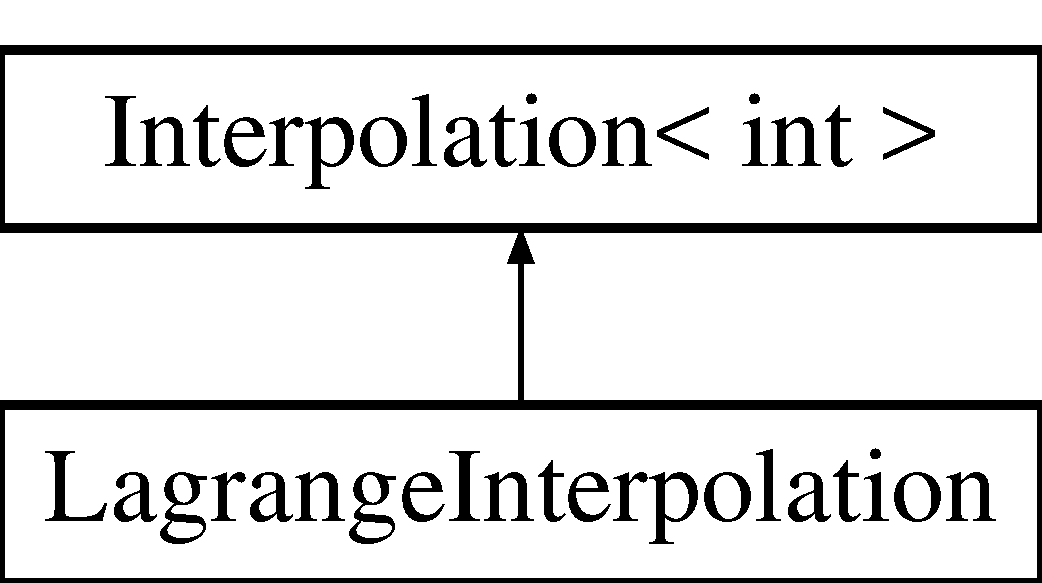
\includegraphics[height=2.000000cm]{class_lagrange_interpolation}
\end{center}
\end{figure}
\subsection*{Public Member Functions}
\begin{DoxyCompactItemize}
\item 
\hyperlink{class_lagrange_interpolation_a706178734a56c65a34c3437fa90aadd5}{Lagrange\+Interpolation} (Functions\+Ptr f, int n\+Iter)
\item 
\hyperlink{class_multi_variate_point}{Multi\+Variate\+Point}$<$ double $>$ \hyperlink{class_lagrange_interpolation_a37a0077fbf7dfa02811e4012cea87f05}{get\+Point} (Multi\+Variate\+Point\+Ptr$<$ int $>$ nu)
\item 
void \hyperlink{class_lagrange_interpolation_ae821197c9a472d99e9b7635db24fbf2b}{add\+Interpolation\+Point} (\hyperlink{class_multi_variate_point}{Multi\+Variate\+Point}$<$ double $>$ p)
\item 
Multi\+Variate\+Point\+Ptr$<$ int $>$ \hyperlink{class_lagrange_interpolation_a6d491cb766b505eee8d65038a6ff6e02}{get\+First\+Multivariate\+Point} ()
\item 
Multi\+Variate\+Point\+Ptr$<$ int $>$ \hyperlink{class_lagrange_interpolation_ac4c9a2d839db489c85ac8818b4abc777}{max\+Element} (int iteration)
\item 
bool \hyperlink{class_lagrange_interpolation_a4e86ab1204fa39cd83b6de4bba621203}{indice\+In\+Path} (\hyperlink{class_multi_variate_point}{Multi\+Variate\+Point}$<$ int $>$ index)
\item 
void \hyperlink{class_lagrange_interpolation_a1e263cf7d5f4ac2272e589a563a53223}{update\+Curent\+Neighbours} (Multi\+Variate\+Point\+Ptr$<$ int $>$ nu)
\item 
bool \hyperlink{class_lagrange_interpolation_ab964d7da47797afd51edf7c82365a17b}{is\+Correct\+Neighbour\+To\+Curent\+Path} (Multi\+Variate\+Point\+Ptr$<$ int $>$ nu)
\item 
double \hyperlink{class_lagrange_interpolation_a138b1d9afd24ab2e21e8c01dac82880c}{basis\+Function\+\_\+1D} (int code, double t, int axis)
\end{DoxyCompactItemize}
\subsection*{Additional Inherited Members}


\subsection{Constructor \& Destructor Documentation}
\index{Lagrange\+Interpolation@{Lagrange\+Interpolation}!Lagrange\+Interpolation@{Lagrange\+Interpolation}}
\index{Lagrange\+Interpolation@{Lagrange\+Interpolation}!Lagrange\+Interpolation@{Lagrange\+Interpolation}}
\subsubsection[{\texorpdfstring{Lagrange\+Interpolation(\+Functions\+Ptr f, int n\+Iter)}{LagrangeInterpolation(FunctionsPtr f, int nIter)}}]{\setlength{\rightskip}{0pt plus 5cm}Lagrange\+Interpolation\+::\+Lagrange\+Interpolation (
\begin{DoxyParamCaption}
\item[{Functions\+Ptr}]{f, }
\item[{int}]{n\+Iter}
\end{DoxyParamCaption}
)}\hypertarget{class_lagrange_interpolation_a706178734a56c65a34c3437fa90aadd5}{}\label{class_lagrange_interpolation_a706178734a56c65a34c3437fa90aadd5}
Constructeur 
\begin{DoxyParams}{Parameters}
{\em f} & \+: fonction à interpoler \\
\hline
{\em n\+Iter} & \+: nombre d\textquotesingle{}itérations dans l\textquotesingle{}algorithme AI \\
\hline
\end{DoxyParams}


\subsection{Member Function Documentation}
\index{Lagrange\+Interpolation@{Lagrange\+Interpolation}!add\+Interpolation\+Point@{add\+Interpolation\+Point}}
\index{add\+Interpolation\+Point@{add\+Interpolation\+Point}!Lagrange\+Interpolation@{Lagrange\+Interpolation}}
\subsubsection[{\texorpdfstring{add\+Interpolation\+Point(\+Multi\+Variate\+Point$<$ double $>$ p)}{addInterpolationPoint(MultiVariatePoint< double > p)}}]{\setlength{\rightskip}{0pt plus 5cm}void Lagrange\+Interpolation\+::add\+Interpolation\+Point (
\begin{DoxyParamCaption}
\item[{{\bf Multi\+Variate\+Point}$<$ double $>$}]{p}
\end{DoxyParamCaption}
)\hspace{0.3cm}{\ttfamily [virtual]}}\hypertarget{class_lagrange_interpolation_ae821197c9a472d99e9b7635db24fbf2b}{}\label{class_lagrange_interpolation_ae821197c9a472d99e9b7635db24fbf2b}
Ajoute le nouveau point d\textquotesingle{}interpolation p dans m\+\_\+interpolation\+Points et m\+\_\+interpolation\+Nodes 
\begin{DoxyParams}{Parameters}
{\em p} & \+: nouveau point d\textquotesingle{}interpolation \\
\hline
\end{DoxyParams}


Implements \hyperlink{class_interpolation_aa2cd083f061f9c36750191da4466c665}{Interpolation$<$ int $>$}.

\index{Lagrange\+Interpolation@{Lagrange\+Interpolation}!basis\+Function\+\_\+1D@{basis\+Function\+\_\+1D}}
\index{basis\+Function\+\_\+1D@{basis\+Function\+\_\+1D}!Lagrange\+Interpolation@{Lagrange\+Interpolation}}
\subsubsection[{\texorpdfstring{basis\+Function\+\_\+1\+D(int code, double t, int axis)}{basisFunction_1D(int code, double t, int axis)}}]{\setlength{\rightskip}{0pt plus 5cm}double Lagrange\+Interpolation\+::basis\+Function\+\_\+1D (
\begin{DoxyParamCaption}
\item[{int}]{code, }
\item[{double}]{t, }
\item[{int}]{axis}
\end{DoxyParamCaption}
)\hspace{0.3cm}{\ttfamily [virtual]}}\hypertarget{class_lagrange_interpolation_a138b1d9afd24ab2e21e8c01dac82880c}{}\label{class_lagrange_interpolation_a138b1d9afd24ab2e21e8c01dac82880c}
Implémente la fonction de base (polynome de Lagrange global) 
\begin{DoxyParams}{Parameters}
{\em code} & \+: indice correspondant à une coordonnée d\textquotesingle{}un point d\textquotesingle{}interpolation \\
\hline
{\em t} & \+: point d\textquotesingle{}évaluation (1d) \\
\hline
{\em axis} & \+: direction concidéré (0 $<$= axis $<$= d-\/1) \\
\hline
\end{DoxyParams}
\begin{DoxyReturn}{Returns}
la valeur au point t de la fonction de base correspondant au point 1d d\textquotesingle{}indice code sur la direction axis 
\end{DoxyReturn}


Implements \hyperlink{class_interpolation_a6a07152ada5102c8b9a9ed88fa46a418}{Interpolation$<$ int $>$}.

\index{Lagrange\+Interpolation@{Lagrange\+Interpolation}!get\+First\+Multivariate\+Point@{get\+First\+Multivariate\+Point}}
\index{get\+First\+Multivariate\+Point@{get\+First\+Multivariate\+Point}!Lagrange\+Interpolation@{Lagrange\+Interpolation}}
\subsubsection[{\texorpdfstring{get\+First\+Multivariate\+Point()}{getFirstMultivariatePoint()}}]{\setlength{\rightskip}{0pt plus 5cm}Multi\+Variate\+Point\+Ptr$<$int$>$ Lagrange\+Interpolation\+::get\+First\+Multivariate\+Point (
\begin{DoxyParamCaption}
{}
\end{DoxyParamCaption}
)\hspace{0.3cm}{\ttfamily [virtual]}}\hypertarget{class_lagrange_interpolation_a6d491cb766b505eee8d65038a6ff6e02}{}\label{class_lagrange_interpolation_a6d491cb766b505eee8d65038a6ff6e02}
Retourner le premier multi-\/indice dans l\textquotesingle{}algo AI \begin{DoxyReturn}{Returns}
le premier multi-\/indice dans l\textquotesingle{}algo AI = (0,..,0) correspont au point multivarié (1.\+0, .., 1.\+0) 
\end{DoxyReturn}


Implements \hyperlink{class_interpolation_ac478b76075519faac66590e9e0df80f5}{Interpolation$<$ int $>$}.

\index{Lagrange\+Interpolation@{Lagrange\+Interpolation}!get\+Point@{get\+Point}}
\index{get\+Point@{get\+Point}!Lagrange\+Interpolation@{Lagrange\+Interpolation}}
\subsubsection[{\texorpdfstring{get\+Point(\+Multi\+Variate\+Point\+Ptr$<$ int $>$ nu)}{getPoint(MultiVariatePointPtr< int > nu)}}]{\setlength{\rightskip}{0pt plus 5cm}{\bf Multi\+Variate\+Point}$<$double$>$ Lagrange\+Interpolation\+::get\+Point (
\begin{DoxyParamCaption}
\item[{Multi\+Variate\+Point\+Ptr$<$ int $>$}]{nu}
\end{DoxyParamCaption}
)\hspace{0.3cm}{\ttfamily [virtual]}}\hypertarget{class_lagrange_interpolation_a37a0077fbf7dfa02811e4012cea87f05}{}\label{class_lagrange_interpolation_a37a0077fbf7dfa02811e4012cea87f05}
Retourne le point multivarié correspondant au multi-\/indice nu 
\begin{DoxyParams}{Parameters}
{\em nu} & \+: mult-\/indice (indice du point 1d de Leja sur chaque direction) \\
\hline
\end{DoxyParams}
\begin{DoxyReturn}{Returns}
point multivarié correspondant à nu 
\end{DoxyReturn}


Implements \hyperlink{class_interpolation_a88593453ec6ce21d53071ddd5bb52195}{Interpolation$<$ int $>$}.

\index{Lagrange\+Interpolation@{Lagrange\+Interpolation}!indice\+In\+Path@{indice\+In\+Path}}
\index{indice\+In\+Path@{indice\+In\+Path}!Lagrange\+Interpolation@{Lagrange\+Interpolation}}
\subsubsection[{\texorpdfstring{indice\+In\+Path(\+Multi\+Variate\+Point$<$ int $>$ index)}{indiceInPath(MultiVariatePoint< int > index)}}]{\setlength{\rightskip}{0pt plus 5cm}bool Lagrange\+Interpolation\+::indice\+In\+Path (
\begin{DoxyParamCaption}
\item[{{\bf Multi\+Variate\+Point}$<$ int $>$}]{index}
\end{DoxyParamCaption}
)\hspace{0.3cm}{\ttfamily [virtual]}}\hypertarget{class_lagrange_interpolation_a4e86ab1204fa39cd83b6de4bba621203}{}\label{class_lagrange_interpolation_a4e86ab1204fa39cd83b6de4bba621203}
Vérifier si le multi-\/indice index existe dans m\+\_\+path (correspond à un point d\textquotesingle{}interpolation) 
\begin{DoxyParams}{Parameters}
{\em index} & multi-\/indice \\
\hline
\end{DoxyParams}
\begin{DoxyReturn}{Returns}
true si et seulement si index est dans m\+\_\+path 
\end{DoxyReturn}


Implements \hyperlink{class_interpolation_a0f2153a7dbc31a1471816a9c6c32eff1}{Interpolation$<$ int $>$}.

\index{Lagrange\+Interpolation@{Lagrange\+Interpolation}!is\+Correct\+Neighbour\+To\+Curent\+Path@{is\+Correct\+Neighbour\+To\+Curent\+Path}}
\index{is\+Correct\+Neighbour\+To\+Curent\+Path@{is\+Correct\+Neighbour\+To\+Curent\+Path}!Lagrange\+Interpolation@{Lagrange\+Interpolation}}
\subsubsection[{\texorpdfstring{is\+Correct\+Neighbour\+To\+Curent\+Path(\+Multi\+Variate\+Point\+Ptr$<$ int $>$ nu)}{isCorrectNeighbourToCurentPath(MultiVariatePointPtr< int > nu)}}]{\setlength{\rightskip}{0pt plus 5cm}bool Lagrange\+Interpolation\+::is\+Correct\+Neighbour\+To\+Curent\+Path (
\begin{DoxyParamCaption}
\item[{Multi\+Variate\+Point\+Ptr$<$ int $>$}]{nu}
\end{DoxyParamCaption}
)\hspace{0.3cm}{\ttfamily [virtual]}}\hypertarget{class_lagrange_interpolation_ab964d7da47797afd51edf7c82365a17b}{}\label{class_lagrange_interpolation_ab964d7da47797afd51edf7c82365a17b}
Vérifier si nu est bien un voisin de la séquence de points d\textquotesingle{}interpolation courante (vérifier la monotonie de l\textquotesingle{}ensemble de points choisis) 
\begin{DoxyParams}{Parameters}
{\em nu} & vecteur d\textquotesingle{}ordre \\
\hline
\end{DoxyParams}
\begin{DoxyReturn}{Returns}
true si et seulement si nu est voisin à l\textquotesingle{}ensemble de points de m\+\_\+path 
\end{DoxyReturn}


Implements \hyperlink{class_interpolation_a3a6ee60651baf1ee8adcd4b874a71523}{Interpolation$<$ int $>$}.

\index{Lagrange\+Interpolation@{Lagrange\+Interpolation}!max\+Element@{max\+Element}}
\index{max\+Element@{max\+Element}!Lagrange\+Interpolation@{Lagrange\+Interpolation}}
\subsubsection[{\texorpdfstring{max\+Element(int iteration)}{maxElement(int iteration)}}]{\setlength{\rightskip}{0pt plus 5cm}Multi\+Variate\+Point\+Ptr$<$int$>$ Lagrange\+Interpolation\+::max\+Element (
\begin{DoxyParamCaption}
\item[{int}]{iteration}
\end{DoxyParamCaption}
)\hspace{0.3cm}{\ttfamily [virtual]}}\hypertarget{class_lagrange_interpolation_ac4c9a2d839db489c85ac8818b4abc777}{}\label{class_lagrange_interpolation_ac4c9a2d839db489c85ac8818b4abc777}
Retourner le vecteur d\textquotesingle{}ordres du prochain point d\textquotesingle{}interpolation sélectionné par l\textquotesingle{}algo AI 3 fois sur 4\+: on choisi celui ayant la plus grande erreur (algo AI) 1 fois sur 4\+: on choisi celui qui a attendu le plus longtemps pour éviter de bloquer une direction dans le cas où l\textquotesingle{}erreur vaut 0 
\begin{DoxyParams}{Parameters}
{\em iteration} & \+: numéro de l\textquotesingle{}itération courante \\
\hline
\end{DoxyParams}
\begin{DoxyReturn}{Returns}
teration \+: vecteur d\textquotesingle{}ordres du prochain point d\textquotesingle{}interpolation 
\end{DoxyReturn}


Implements \hyperlink{class_interpolation_a92dcf9a209d2a8046b266b59811949d4}{Interpolation$<$ int $>$}.

\index{Lagrange\+Interpolation@{Lagrange\+Interpolation}!update\+Curent\+Neighbours@{update\+Curent\+Neighbours}}
\index{update\+Curent\+Neighbours@{update\+Curent\+Neighbours}!Lagrange\+Interpolation@{Lagrange\+Interpolation}}
\subsubsection[{\texorpdfstring{update\+Curent\+Neighbours(\+Multi\+Variate\+Point\+Ptr$<$ int $>$ nu)}{updateCurentNeighbours(MultiVariatePointPtr< int > nu)}}]{\setlength{\rightskip}{0pt plus 5cm}void Lagrange\+Interpolation\+::update\+Curent\+Neighbours (
\begin{DoxyParamCaption}
\item[{Multi\+Variate\+Point\+Ptr$<$ int $>$}]{nu}
\end{DoxyParamCaption}
)\hspace{0.3cm}{\ttfamily [virtual]}}\hypertarget{class_lagrange_interpolation_a1e263cf7d5f4ac2272e589a563a53223}{}\label{class_lagrange_interpolation_a1e263cf7d5f4ac2272e589a563a53223}
Mettre à jour, en fonction du nouveau point d\textquotesingle{}interpolation correspondant au multi-\/indice nu, la liste des candidats courant 
\begin{DoxyParams}{Parameters}
{\em nu} & nouveau multi-\/indices choisi par l\textquotesingle{}algo AI \\
\hline
\end{DoxyParams}


Implements \hyperlink{class_interpolation_ac2e37b60de1c7b6704be643563fedd91}{Interpolation$<$ int $>$}.



The documentation for this class was generated from the following file\+:\begin{DoxyCompactItemize}
\item 
include/\hyperlink{_lagrange_interpolation_8hpp}{Lagrange\+Interpolation.\+hpp}\end{DoxyCompactItemize}

\hypertarget{class_mixed_interpolation}{}\section{Mixed\+Interpolation Class Reference}
\label{class_mixed_interpolation}\index{Mixed\+Interpolation@{Mixed\+Interpolation}}
Inheritance diagram for Mixed\+Interpolation\+:\begin{figure}[H]
\begin{center}
\leavevmode
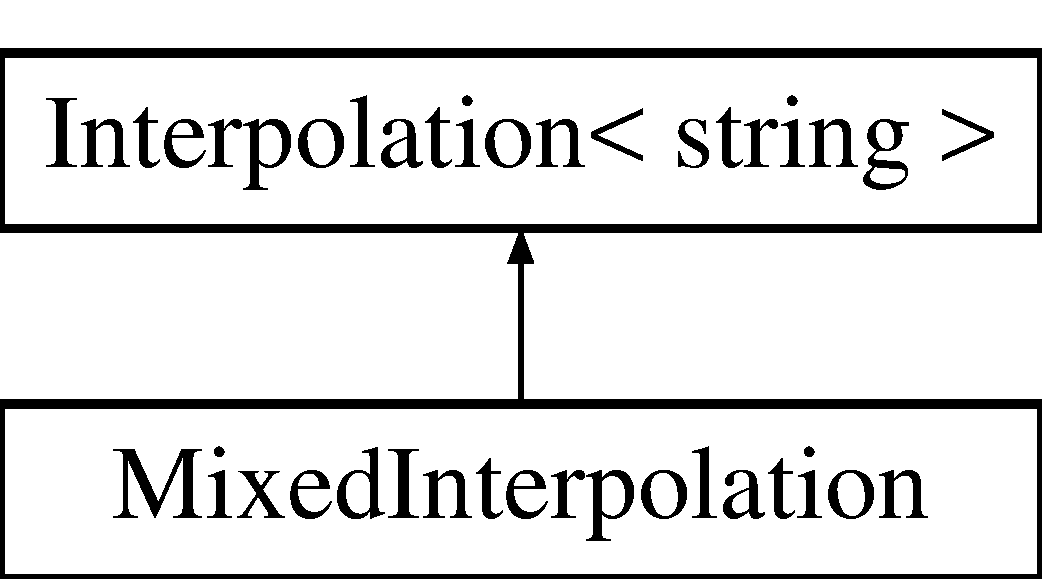
\includegraphics[height=2.000000cm]{class_mixed_interpolation}
\end{center}
\end{figure}
\subsection*{Public Member Functions}
\begin{DoxyCompactItemize}
\item 
\hyperlink{class_mixed_interpolation_a5cf10a29fd266fe64811b2898b71af32}{Mixed\+Interpolation} (Functions\+Ptr f, int n\+Iter, \hyperlink{class_multi_variate_point}{Multi\+Variate\+Point}$<$ int $>$ methods)
\item 
void \hyperlink{class_mixed_interpolation_a269665fad93a49651d2d519d581efd49}{set\+Methods} (\hyperlink{class_multi_variate_point}{Multi\+Variate\+Point}$<$ int $>$ methods)
\item 
void \hyperlink{class_mixed_interpolation_a665be96aea549b82d877d1fc8eff1a9b}{clear\+All\+Trees} ()
\item 
\hyperlink{class_multi_variate_point}{Multi\+Variate\+Point}$<$ double $>$ \hyperlink{class_mixed_interpolation_a545bde4e4c83d9806fd08a6891b07af7}{get\+Point} (Multi\+Variate\+Point\+Ptr$<$ string $>$ nu)
\item 
void \hyperlink{class_mixed_interpolation_a51027c6018481bbfa4102901575e32ee}{add\+Interpolation\+Point} (\hyperlink{class_multi_variate_point}{Multi\+Variate\+Point}$<$ double $>$ p)
\item 
Multi\+Variate\+Point\+Ptr$<$ string $>$ \hyperlink{class_mixed_interpolation_a508361e1615e4fb3e77c702617637d6d}{get\+First\+Multivariate\+Point} ()
\item 
Multi\+Variate\+Point\+Ptr$<$ string $>$ \hyperlink{class_mixed_interpolation_a45908a6d89efe869a2b80d9f50264f7f}{max\+Element} (int iteration)
\item 
bool \hyperlink{class_mixed_interpolation_a5009f0fbe969538db58d5fa2f9997e4f}{indice\+In\+Path} (\hyperlink{class_multi_variate_point}{Multi\+Variate\+Point}$<$ string $>$ index)
\item 
void \hyperlink{class_mixed_interpolation_af5bbe4c2c6383989d3869f76ca6467c9}{update\+Curent\+Neighbours} (Multi\+Variate\+Point\+Ptr$<$ string $>$ nu)
\item 
bool \hyperlink{class_mixed_interpolation_af507dcd64c768b97c0ba2ff378a14f91}{is\+Correct\+Neighbour\+To\+Curent\+Path} (Multi\+Variate\+Point\+Ptr$<$ string $>$ nu)
\item 
double \hyperlink{class_mixed_interpolation_a97c5b558e53a5c98ed17d3fad6bb40ad}{basis\+Function\+\_\+1D} (string code, double t, int axis)
\item 
void \hyperlink{class_mixed_interpolation_a11a20252cbe44536f5be6024b348d755}{compute\+Boundaries\+For\+Basis\+Function} (double t, double $\ast$inf, double $\ast$sup, int axis)
\end{DoxyCompactItemize}
\subsection*{Additional Inherited Members}


\subsection{Constructor \& Destructor Documentation}
\index{Mixed\+Interpolation@{Mixed\+Interpolation}!Mixed\+Interpolation@{Mixed\+Interpolation}}
\index{Mixed\+Interpolation@{Mixed\+Interpolation}!Mixed\+Interpolation@{Mixed\+Interpolation}}
\subsubsection[{\texorpdfstring{Mixed\+Interpolation(\+Functions\+Ptr f, int n\+Iter, Multi\+Variate\+Point$<$ int $>$ methods)}{MixedInterpolation(FunctionsPtr f, int nIter, MultiVariatePoint< int > methods)}}]{\setlength{\rightskip}{0pt plus 5cm}Mixed\+Interpolation\+::\+Mixed\+Interpolation (
\begin{DoxyParamCaption}
\item[{Functions\+Ptr}]{f, }
\item[{int}]{n\+Iter, }
\item[{{\bf Multi\+Variate\+Point}$<$ int $>$}]{methods}
\end{DoxyParamCaption}
)}\hypertarget{class_mixed_interpolation_a5cf10a29fd266fe64811b2898b71af32}{}\label{class_mixed_interpolation_a5cf10a29fd266fe64811b2898b71af32}
Constructeur 
\begin{DoxyParams}{Parameters}
{\em f} & \+: fonction à interpoler \\
\hline
{\em n\+Iter} & \+: nombre d\textquotesingle{}itérations dans l\textquotesingle{}algorithme AI \\
\hline
{\em methods} & \+: indique la version utilisée par l\textquotesingle{}algorithme AI dans chaque direction \\
\hline
\end{DoxyParams}


\subsection{Member Function Documentation}
\index{Mixed\+Interpolation@{Mixed\+Interpolation}!add\+Interpolation\+Point@{add\+Interpolation\+Point}}
\index{add\+Interpolation\+Point@{add\+Interpolation\+Point}!Mixed\+Interpolation@{Mixed\+Interpolation}}
\subsubsection[{\texorpdfstring{add\+Interpolation\+Point(\+Multi\+Variate\+Point$<$ double $>$ p)}{addInterpolationPoint(MultiVariatePoint< double > p)}}]{\setlength{\rightskip}{0pt plus 5cm}void Mixed\+Interpolation\+::add\+Interpolation\+Point (
\begin{DoxyParamCaption}
\item[{{\bf Multi\+Variate\+Point}$<$ double $>$}]{p}
\end{DoxyParamCaption}
)\hspace{0.3cm}{\ttfamily [virtual]}}\hypertarget{class_mixed_interpolation_a51027c6018481bbfa4102901575e32ee}{}\label{class_mixed_interpolation_a51027c6018481bbfa4102901575e32ee}
Ajoute le nouveau point d\textquotesingle{}interpolation p dans m\+\_\+interpolation\+Points, m\+\_\+interpolation\+Nodes et m\+\_\+trees 
\begin{DoxyParams}{Parameters}
{\em p} & \+: nouveau point d\textquotesingle{}interpolation \\
\hline
\end{DoxyParams}


Implements \hyperlink{class_interpolation_aa2cd083f061f9c36750191da4466c665}{Interpolation$<$ string $>$}.

\index{Mixed\+Interpolation@{Mixed\+Interpolation}!basis\+Function\+\_\+1D@{basis\+Function\+\_\+1D}}
\index{basis\+Function\+\_\+1D@{basis\+Function\+\_\+1D}!Mixed\+Interpolation@{Mixed\+Interpolation}}
\subsubsection[{\texorpdfstring{basis\+Function\+\_\+1\+D(string code, double t, int axis)}{basisFunction_1D(string code, double t, int axis)}}]{\setlength{\rightskip}{0pt plus 5cm}double Mixed\+Interpolation\+::basis\+Function\+\_\+1D (
\begin{DoxyParamCaption}
\item[{string}]{code, }
\item[{double}]{t, }
\item[{int}]{axis}
\end{DoxyParamCaption}
)\hspace{0.3cm}{\ttfamily [virtual]}}\hypertarget{class_mixed_interpolation_a97c5b558e53a5c98ed17d3fad6bb40ad}{}\label{class_mixed_interpolation_a97c5b558e53a5c98ed17d3fad6bb40ad}
Implémente la fonction de base (polynome de Lagrange global, fonction affine (ou quadratique) par morceaux (dépend de la version de l\textquotesingle{}algo AI) 
\begin{DoxyParams}{Parameters}
{\em code} & \+: ordre (indice ou code de Huffman) correspondant à une coordonnée d\textquotesingle{}un point d\textquotesingle{}interpolation \\
\hline
{\em t} & \+: point d\textquotesingle{}évaluation (1d) \\
\hline
{\em axis} & \+: direction concidéré (0 $<$= axis $<$= d-\/1) \\
\hline
\end{DoxyParams}
\begin{DoxyReturn}{Returns}
la valeur au point t de la fonction de base correspondant au point 1d d\textquotesingle{}ordre code sur la direction axis 
\end{DoxyReturn}


Implements \hyperlink{class_interpolation_a6a07152ada5102c8b9a9ed88fa46a418}{Interpolation$<$ string $>$}.

\index{Mixed\+Interpolation@{Mixed\+Interpolation}!clear\+All\+Trees@{clear\+All\+Trees}}
\index{clear\+All\+Trees@{clear\+All\+Trees}!Mixed\+Interpolation@{Mixed\+Interpolation}}
\subsubsection[{\texorpdfstring{clear\+All\+Trees()}{clearAllTrees()}}]{\setlength{\rightskip}{0pt plus 5cm}void Mixed\+Interpolation\+::clear\+All\+Trees (
\begin{DoxyParamCaption}
{}
\end{DoxyParamCaption}
)}\hypertarget{class_mixed_interpolation_a665be96aea549b82d877d1fc8eff1a9b}{}\label{class_mixed_interpolation_a665be96aea549b82d877d1fc8eff1a9b}
Supprimer tous les arbres de m\+\_\+trees \index{Mixed\+Interpolation@{Mixed\+Interpolation}!compute\+Boundaries\+For\+Basis\+Function@{compute\+Boundaries\+For\+Basis\+Function}}
\index{compute\+Boundaries\+For\+Basis\+Function@{compute\+Boundaries\+For\+Basis\+Function}!Mixed\+Interpolation@{Mixed\+Interpolation}}
\subsubsection[{\texorpdfstring{compute\+Boundaries\+For\+Basis\+Function(double t, double $\ast$inf, double $\ast$sup, int axis)}{computeBoundariesForBasisFunction(double t, double *inf, double *sup, int axis)}}]{\setlength{\rightskip}{0pt plus 5cm}void Mixed\+Interpolation\+::compute\+Boundaries\+For\+Basis\+Function (
\begin{DoxyParamCaption}
\item[{double}]{t, }
\item[{double $\ast$}]{inf, }
\item[{double $\ast$}]{sup, }
\item[{int}]{axis}
\end{DoxyParamCaption}
)}\hypertarget{class_mixed_interpolation_a11a20252cbe44536f5be6024b348d755}{}\label{class_mixed_interpolation_a11a20252cbe44536f5be6024b348d755}
Rechercher les valeurs des points d\textquotesingle{}interpolation 1d (inf et sup) les plus proches de t (de part et d\textquotesingle{}autre de t) sur la direction axis pour construire la fonction de base 
\begin{DoxyParams}{Parameters}
{\em t} & \+: point d\textquotesingle{}interpolation 1d \\
\hline
{\em inf} & \+: plus grand point d\textquotesingle{}interpolation 1d inférieur à t \\
\hline
{\em sup} & \+: plus petit point d\textquotesingle{}interpolation 1d supérieur à t \\
\hline
{\em axis} & \+: direction concidérée \\
\hline
\end{DoxyParams}
\index{Mixed\+Interpolation@{Mixed\+Interpolation}!get\+First\+Multivariate\+Point@{get\+First\+Multivariate\+Point}}
\index{get\+First\+Multivariate\+Point@{get\+First\+Multivariate\+Point}!Mixed\+Interpolation@{Mixed\+Interpolation}}
\subsubsection[{\texorpdfstring{get\+First\+Multivariate\+Point()}{getFirstMultivariatePoint()}}]{\setlength{\rightskip}{0pt plus 5cm}Multi\+Variate\+Point\+Ptr$<$string$>$ Mixed\+Interpolation\+::get\+First\+Multivariate\+Point (
\begin{DoxyParamCaption}
{}
\end{DoxyParamCaption}
)\hspace{0.3cm}{\ttfamily [virtual]}}\hypertarget{class_mixed_interpolation_a508361e1615e4fb3e77c702617637d6d}{}\label{class_mixed_interpolation_a508361e1615e4fb3e77c702617637d6d}
Retourner le premier vecteur d\textquotesingle{}ordres dans l\textquotesingle{}algo AI \begin{DoxyReturn}{Returns}
le premier vecteur d\textquotesingle{}ordres (codes de Huffman ou indice de point de Leja) dans l\textquotesingle{}algo AI 
\end{DoxyReturn}


Implements \hyperlink{class_interpolation_ac478b76075519faac66590e9e0df80f5}{Interpolation$<$ string $>$}.

\index{Mixed\+Interpolation@{Mixed\+Interpolation}!get\+Point@{get\+Point}}
\index{get\+Point@{get\+Point}!Mixed\+Interpolation@{Mixed\+Interpolation}}
\subsubsection[{\texorpdfstring{get\+Point(\+Multi\+Variate\+Point\+Ptr$<$ string $>$ nu)}{getPoint(MultiVariatePointPtr< string > nu)}}]{\setlength{\rightskip}{0pt plus 5cm}{\bf Multi\+Variate\+Point}$<$double$>$ Mixed\+Interpolation\+::get\+Point (
\begin{DoxyParamCaption}
\item[{Multi\+Variate\+Point\+Ptr$<$ string $>$}]{nu}
\end{DoxyParamCaption}
)\hspace{0.3cm}{\ttfamily [virtual]}}\hypertarget{class_mixed_interpolation_a545bde4e4c83d9806fd08a6891b07af7}{}\label{class_mixed_interpolation_a545bde4e4c83d9806fd08a6891b07af7}
Retourne le point multivarié correspondant au vecteur d\textquotesingle{}ordres nu 
\begin{DoxyParams}{Parameters}
{\em nu} & \+: vecteur contenant des codes de Huffman (chemin du point 1d dans l\textquotesingle{}arbre binaire) ou des indices (indice du point 1d de Leja) sur chaque direction \\
\hline
\end{DoxyParams}
\begin{DoxyReturn}{Returns}
point multivarié correspondant à nu 
\end{DoxyReturn}


Implements \hyperlink{class_interpolation_a88593453ec6ce21d53071ddd5bb52195}{Interpolation$<$ string $>$}.

\index{Mixed\+Interpolation@{Mixed\+Interpolation}!indice\+In\+Path@{indice\+In\+Path}}
\index{indice\+In\+Path@{indice\+In\+Path}!Mixed\+Interpolation@{Mixed\+Interpolation}}
\subsubsection[{\texorpdfstring{indice\+In\+Path(\+Multi\+Variate\+Point$<$ string $>$ index)}{indiceInPath(MultiVariatePoint< string > index)}}]{\setlength{\rightskip}{0pt plus 5cm}bool Mixed\+Interpolation\+::indice\+In\+Path (
\begin{DoxyParamCaption}
\item[{{\bf Multi\+Variate\+Point}$<$ string $>$}]{index}
\end{DoxyParamCaption}
)\hspace{0.3cm}{\ttfamily [virtual]}}\hypertarget{class_mixed_interpolation_a5009f0fbe969538db58d5fa2f9997e4f}{}\label{class_mixed_interpolation_a5009f0fbe969538db58d5fa2f9997e4f}
Vérifier si le vecteur d\textquotesingle{}ordre (codes de Huffman, ou indices) index existe dans m\+\_\+path (correspond à un point d\textquotesingle{}interpolation) 
\begin{DoxyParams}{Parameters}
{\em index} & \+: vecteur d\textquotesingle{}ordres \\
\hline
\end{DoxyParams}
\begin{DoxyReturn}{Returns}
true si et seulement si index est dans m\+\_\+path 
\end{DoxyReturn}


Implements \hyperlink{class_interpolation_a0f2153a7dbc31a1471816a9c6c32eff1}{Interpolation$<$ string $>$}.

\index{Mixed\+Interpolation@{Mixed\+Interpolation}!is\+Correct\+Neighbour\+To\+Curent\+Path@{is\+Correct\+Neighbour\+To\+Curent\+Path}}
\index{is\+Correct\+Neighbour\+To\+Curent\+Path@{is\+Correct\+Neighbour\+To\+Curent\+Path}!Mixed\+Interpolation@{Mixed\+Interpolation}}
\subsubsection[{\texorpdfstring{is\+Correct\+Neighbour\+To\+Curent\+Path(\+Multi\+Variate\+Point\+Ptr$<$ string $>$ nu)}{isCorrectNeighbourToCurentPath(MultiVariatePointPtr< string > nu)}}]{\setlength{\rightskip}{0pt plus 5cm}bool Mixed\+Interpolation\+::is\+Correct\+Neighbour\+To\+Curent\+Path (
\begin{DoxyParamCaption}
\item[{Multi\+Variate\+Point\+Ptr$<$ string $>$}]{nu}
\end{DoxyParamCaption}
)\hspace{0.3cm}{\ttfamily [virtual]}}\hypertarget{class_mixed_interpolation_af507dcd64c768b97c0ba2ff378a14f91}{}\label{class_mixed_interpolation_af507dcd64c768b97c0ba2ff378a14f91}
Vérifier si nu est bien un voisin de la séquence de points d\textquotesingle{}interpolation courante (vérifier la monotonie de l\textquotesingle{}ensemble de points choisis) 
\begin{DoxyParams}{Parameters}
{\em nu} & \+: vecteur d\textquotesingle{}ordre \\
\hline
\end{DoxyParams}
\begin{DoxyReturn}{Returns}
true si et seulement si nu est voisin à l\textquotesingle{}ensemble de points de m\+\_\+path 
\end{DoxyReturn}


Implements \hyperlink{class_interpolation_a3a6ee60651baf1ee8adcd4b874a71523}{Interpolation$<$ string $>$}.

\index{Mixed\+Interpolation@{Mixed\+Interpolation}!max\+Element@{max\+Element}}
\index{max\+Element@{max\+Element}!Mixed\+Interpolation@{Mixed\+Interpolation}}
\subsubsection[{\texorpdfstring{max\+Element(int iteration)}{maxElement(int iteration)}}]{\setlength{\rightskip}{0pt plus 5cm}Multi\+Variate\+Point\+Ptr$<$string$>$ Mixed\+Interpolation\+::max\+Element (
\begin{DoxyParamCaption}
\item[{int}]{iteration}
\end{DoxyParamCaption}
)\hspace{0.3cm}{\ttfamily [virtual]}}\hypertarget{class_mixed_interpolation_a45908a6d89efe869a2b80d9f50264f7f}{}\label{class_mixed_interpolation_a45908a6d89efe869a2b80d9f50264f7f}
Retourner le vecteur d\textquotesingle{}ordres du prochain point d\textquotesingle{}interpolation sélectionné par l\textquotesingle{}algo AI 3 fois sur 4\+: on choisi celui ayant la plus grande erreur (algo AI) 1 fois sur 4\+: on choisi celui qui a attendu le plus longtemps pour éviter de bloquer une direction dans le cas où l\textquotesingle{}erreur vaut 0 
\begin{DoxyParams}{Parameters}
{\em iteration} & \+: numéro de l\textquotesingle{}itération courante \\
\hline
\end{DoxyParams}
\begin{DoxyReturn}{Returns}
teration \+: vecteur d\textquotesingle{}ordres du prochain point d\textquotesingle{}interpolation 
\end{DoxyReturn}


Implements \hyperlink{class_interpolation_a92dcf9a209d2a8046b266b59811949d4}{Interpolation$<$ string $>$}.

\index{Mixed\+Interpolation@{Mixed\+Interpolation}!set\+Methods@{set\+Methods}}
\index{set\+Methods@{set\+Methods}!Mixed\+Interpolation@{Mixed\+Interpolation}}
\subsubsection[{\texorpdfstring{set\+Methods(\+Multi\+Variate\+Point$<$ int $>$ methods)}{setMethods(MultiVariatePoint< int > methods)}}]{\setlength{\rightskip}{0pt plus 5cm}void Mixed\+Interpolation\+::set\+Methods (
\begin{DoxyParamCaption}
\item[{{\bf Multi\+Variate\+Point}$<$ int $>$}]{methods}
\end{DoxyParamCaption}
)\hspace{0.3cm}{\ttfamily [inline]}}\hypertarget{class_mixed_interpolation_a269665fad93a49651d2d519d581efd49}{}\label{class_mixed_interpolation_a269665fad93a49651d2d519d581efd49}
Mutateur de l\textquotesingle{}attribut m\+\_\+methods param methods \+: liste des versions utilisées sur chaque directions \index{Mixed\+Interpolation@{Mixed\+Interpolation}!update\+Curent\+Neighbours@{update\+Curent\+Neighbours}}
\index{update\+Curent\+Neighbours@{update\+Curent\+Neighbours}!Mixed\+Interpolation@{Mixed\+Interpolation}}
\subsubsection[{\texorpdfstring{update\+Curent\+Neighbours(\+Multi\+Variate\+Point\+Ptr$<$ string $>$ nu)}{updateCurentNeighbours(MultiVariatePointPtr< string > nu)}}]{\setlength{\rightskip}{0pt plus 5cm}void Mixed\+Interpolation\+::update\+Curent\+Neighbours (
\begin{DoxyParamCaption}
\item[{Multi\+Variate\+Point\+Ptr$<$ string $>$}]{nu}
\end{DoxyParamCaption}
)\hspace{0.3cm}{\ttfamily [virtual]}}\hypertarget{class_mixed_interpolation_af5bbe4c2c6383989d3869f76ca6467c9}{}\label{class_mixed_interpolation_af5bbe4c2c6383989d3869f76ca6467c9}
Mettre à jour, en fonction du nouveau point d\textquotesingle{}interpolation correspondant au vecteur d\textquotesingle{}ordre nu, la liste des candidats courant 
\begin{DoxyParams}{Parameters}
{\em nu} & \+: nouveau vecteur d\textquotesingle{}ordre choisi par l\textquotesingle{}algo AI \\
\hline
\end{DoxyParams}


Implements \hyperlink{class_interpolation_ac2e37b60de1c7b6704be643563fedd91}{Interpolation$<$ string $>$}.



The documentation for this class was generated from the following file\+:\begin{DoxyCompactItemize}
\item 
include/\hyperlink{_mixed_interpolation_8hpp}{Mixed\+Interpolation.\+hpp}\end{DoxyCompactItemize}

\hypertarget{class_multi_variate_point}{}\section{Multi\+Variate\+Point$<$ T $>$ Class Template Reference}
\label{class_multi_variate_point}\index{Multi\+Variate\+Point$<$ T $>$@{Multi\+Variate\+Point$<$ T $>$}}
\subsection*{Public Member Functions}
\begin{DoxyCompactItemize}
\item 
\hyperlink{class_multi_variate_point_a2ab2acda8a5c5289220f130117bd5f95}{Multi\+Variate\+Point} (int d, int n, T val)
\item 
\hyperlink{class_multi_variate_point_ad497f54132498b6141484057d042e157}{Multi\+Variate\+Point} (const \hyperlink{class_multi_variate_point}{Multi\+Variate\+Point}$<$ T $>$ \&nu)
\item 
int \hyperlink{class_multi_variate_point_a32acfceae3008c886b5101a292d16efb}{getD} () const 
\item 
int \hyperlink{class_multi_variate_point_ac3e4878d6202deeb489a7c117799e53b}{getN} () const 
\item 
int \hyperlink{class_multi_variate_point_accf19c239f3359ac9d8d6057a7b913c2}{get\+Nb\+Waiting\+Iter} ()
\item 
void \hyperlink{class_multi_variate_point_aedc8c232c76736f1f5e4a563bf8d4fc4}{incr\+Nb\+Waiting\+Iter} ()
\item 
vector$<$ double $>$ \hyperlink{class_multi_variate_point_ac67af657777f1e7c31b1b5d11df2b788}{get\+Alpha} () const 
\item 
void \hyperlink{class_multi_variate_point_aa7a4e466b5337a6978b5140ca2492545}{set\+Alpha} (vector$<$ double $>$ alpha)
\item 
bool \hyperlink{class_multi_variate_point_a5fa298c0efa8ca27708cb17b82e28316}{alpha\+Already\+Computed} ()
\item 
bool \hyperlink{class_multi_variate_point_a5afa1773c5bdcf30a9b51b29cc4cb6a9}{alpha\+Is\+Null} ()
\item 
void {\bfseries reinit} ()\hypertarget{class_multi_variate_point_aa01525fcdeee3650a5b10e9fd5375671}{}\label{class_multi_variate_point_aa01525fcdeee3650a5b10e9fd5375671}

\item 
T \& {\bfseries operator()} (int d) const \hypertarget{class_multi_variate_point_a1615d3e6f128a882dfa038051b0f3225}{}\label{class_multi_variate_point_a1615d3e6f128a882dfa038051b0f3225}

\item 
\hyperlink{class_multi_variate_point}{Multi\+Variate\+Point} \& {\bfseries operator+=} (const \hyperlink{class_multi_variate_point}{Multi\+Variate\+Point} \&v)\hypertarget{class_multi_variate_point_aa8c0b072bd69e6e5fda6410dfed40f9a}{}\label{class_multi_variate_point_aa8c0b072bd69e6e5fda6410dfed40f9a}

\item 
\hyperlink{class_multi_variate_point}{Multi\+Variate\+Point} \& {\bfseries operator-\/=} (const \hyperlink{class_multi_variate_point}{Multi\+Variate\+Point} \&v)\hypertarget{class_multi_variate_point_aeed522c7d3438f8ce6ee2982383d13c3}{}\label{class_multi_variate_point_aeed522c7d3438f8ce6ee2982383d13c3}

\item 
\hyperlink{class_multi_variate_point}{Multi\+Variate\+Point} \& {\bfseries operator$\ast$=} (const double \&r)\hypertarget{class_multi_variate_point_af2ac0ba60bb5787a3e9d0d7244b358f9}{}\label{class_multi_variate_point_af2ac0ba60bb5787a3e9d0d7244b358f9}

\item 
\hyperlink{class_multi_variate_point}{Multi\+Variate\+Point} \& {\bfseries operator=} (\hyperlink{class_multi_variate_point}{Multi\+Variate\+Point} const \&nu)\hypertarget{class_multi_variate_point_a6cdc125e64fc57bc78e71dbac77e5640}{}\label{class_multi_variate_point_a6cdc125e64fc57bc78e71dbac77e5640}

\end{DoxyCompactItemize}


\subsection{Constructor \& Destructor Documentation}
\index{Multi\+Variate\+Point@{Multi\+Variate\+Point}!Multi\+Variate\+Point@{Multi\+Variate\+Point}}
\index{Multi\+Variate\+Point@{Multi\+Variate\+Point}!Multi\+Variate\+Point@{Multi\+Variate\+Point}}
\subsubsection[{\texorpdfstring{Multi\+Variate\+Point(int d, int n, T val)}{MultiVariatePoint(int d, int n, T val)}}]{\setlength{\rightskip}{0pt plus 5cm}template$<$typename T$>$ {\bf Multi\+Variate\+Point}$<$ T $>$\+::{\bf Multi\+Variate\+Point} (
\begin{DoxyParamCaption}
\item[{int}]{d, }
\item[{int}]{n, }
\item[{T}]{val}
\end{DoxyParamCaption}
)}\hypertarget{class_multi_variate_point_a2ab2acda8a5c5289220f130117bd5f95}{}\label{class_multi_variate_point_a2ab2acda8a5c5289220f130117bd5f95}
Constructeur 
\begin{DoxyParams}{Parameters}
{\em d} & \+: dimension de l\textquotesingle{}éspace de départ de f, (taille du point multivarié) \\
\hline
{\em n} & \+: dimension de l\textquotesingle{}éspace d\textquotesingle{}arrivé de f, (taille de l\textquotesingle{}erreur au point multivarié) \\
\hline
{\em T} & \+: valeur par défaut des coordonnées du point multivariés \\
\hline
\end{DoxyParams}
\index{Multi\+Variate\+Point@{Multi\+Variate\+Point}!Multi\+Variate\+Point@{Multi\+Variate\+Point}}
\index{Multi\+Variate\+Point@{Multi\+Variate\+Point}!Multi\+Variate\+Point@{Multi\+Variate\+Point}}
\subsubsection[{\texorpdfstring{Multi\+Variate\+Point(const Multi\+Variate\+Point$<$ T $>$ \&nu)}{MultiVariatePoint(const MultiVariatePoint< T > &nu)}}]{\setlength{\rightskip}{0pt plus 5cm}template$<$typename T$>$ {\bf Multi\+Variate\+Point}$<$ T $>$\+::{\bf Multi\+Variate\+Point} (
\begin{DoxyParamCaption}
\item[{const {\bf Multi\+Variate\+Point}$<$ T $>$ \&}]{nu}
\end{DoxyParamCaption}
)}\hypertarget{class_multi_variate_point_ad497f54132498b6141484057d042e157}{}\label{class_multi_variate_point_ad497f54132498b6141484057d042e157}
Constructeur par copie 
\begin{DoxyParams}{Parameters}
{\em nu} & \+: point multivarié \\
\hline
\end{DoxyParams}


\subsection{Member Function Documentation}
\index{Multi\+Variate\+Point@{Multi\+Variate\+Point}!alpha\+Already\+Computed@{alpha\+Already\+Computed}}
\index{alpha\+Already\+Computed@{alpha\+Already\+Computed}!Multi\+Variate\+Point@{Multi\+Variate\+Point}}
\subsubsection[{\texorpdfstring{alpha\+Already\+Computed()}{alphaAlreadyComputed()}}]{\setlength{\rightskip}{0pt plus 5cm}template$<$typename T $>$ bool {\bf Multi\+Variate\+Point}$<$ T $>$\+::alpha\+Already\+Computed (
\begin{DoxyParamCaption}
{}
\end{DoxyParamCaption}
)}\hypertarget{class_multi_variate_point_a5fa298c0efa8ca27708cb17b82e28316}{}\label{class_multi_variate_point_a5fa298c0efa8ca27708cb17b82e28316}
Vérifier si m\+\_\+alpha a déjà été calculé (en le comparant à m\+\_\+initial\+Alpha) \begin{DoxyReturn}{Returns}
True si et seulement m\+\_\+alpha != m\+\_\+initial\+Alpha 
\end{DoxyReturn}
\index{Multi\+Variate\+Point@{Multi\+Variate\+Point}!alpha\+Is\+Null@{alpha\+Is\+Null}}
\index{alpha\+Is\+Null@{alpha\+Is\+Null}!Multi\+Variate\+Point@{Multi\+Variate\+Point}}
\subsubsection[{\texorpdfstring{alpha\+Is\+Null()}{alphaIsNull()}}]{\setlength{\rightskip}{0pt plus 5cm}template$<$typename T $>$ bool {\bf Multi\+Variate\+Point}$<$ T $>$\+::alpha\+Is\+Null (
\begin{DoxyParamCaption}
{}
\end{DoxyParamCaption}
)}\hypertarget{class_multi_variate_point_a5afa1773c5bdcf30a9b51b29cc4cb6a9}{}\label{class_multi_variate_point_a5afa1773c5bdcf30a9b51b29cc4cb6a9}
Vérifier si m\+\_\+alpha est nulle \begin{DoxyReturn}{Returns}
True si et seulement si m\+\_\+alpha vaut (0,..,0) 
\end{DoxyReturn}
\index{Multi\+Variate\+Point@{Multi\+Variate\+Point}!get\+Alpha@{get\+Alpha}}
\index{get\+Alpha@{get\+Alpha}!Multi\+Variate\+Point@{Multi\+Variate\+Point}}
\subsubsection[{\texorpdfstring{get\+Alpha() const }{getAlpha() const }}]{\setlength{\rightskip}{0pt plus 5cm}template$<$typename T$>$ vector$<$double$>$ {\bf Multi\+Variate\+Point}$<$ T $>$\+::get\+Alpha (
\begin{DoxyParamCaption}
{}
\end{DoxyParamCaption}
) const\hspace{0.3cm}{\ttfamily [inline]}}\hypertarget{class_multi_variate_point_ac67af657777f1e7c31b1b5d11df2b788}{}\label{class_multi_variate_point_ac67af657777f1e7c31b1b5d11df2b788}
Accesseur à l\textquotesingle{}attribut m\+\_\+alpha \begin{DoxyReturn}{Returns}
valeur de m\+\_\+alpha 
\end{DoxyReturn}
\index{Multi\+Variate\+Point@{Multi\+Variate\+Point}!getD@{getD}}
\index{getD@{getD}!Multi\+Variate\+Point@{Multi\+Variate\+Point}}
\subsubsection[{\texorpdfstring{get\+D() const }{getD() const }}]{\setlength{\rightskip}{0pt plus 5cm}template$<$typename T$>$ int {\bf Multi\+Variate\+Point}$<$ T $>$\+::getD (
\begin{DoxyParamCaption}
{}
\end{DoxyParamCaption}
) const\hspace{0.3cm}{\ttfamily [inline]}}\hypertarget{class_multi_variate_point_a32acfceae3008c886b5101a292d16efb}{}\label{class_multi_variate_point_a32acfceae3008c886b5101a292d16efb}
Accesseur à l\textquotesingle{}attribut m\+\_\+d \begin{DoxyReturn}{Returns}
valeur de m\+\_\+d 
\end{DoxyReturn}
\index{Multi\+Variate\+Point@{Multi\+Variate\+Point}!getN@{getN}}
\index{getN@{getN}!Multi\+Variate\+Point@{Multi\+Variate\+Point}}
\subsubsection[{\texorpdfstring{get\+N() const }{getN() const }}]{\setlength{\rightskip}{0pt plus 5cm}template$<$typename T$>$ int {\bf Multi\+Variate\+Point}$<$ T $>$\+::getN (
\begin{DoxyParamCaption}
{}
\end{DoxyParamCaption}
) const\hspace{0.3cm}{\ttfamily [inline]}}\hypertarget{class_multi_variate_point_ac3e4878d6202deeb489a7c117799e53b}{}\label{class_multi_variate_point_ac3e4878d6202deeb489a7c117799e53b}
Accesseur à l\textquotesingle{}attribut m\+\_\+n \begin{DoxyReturn}{Returns}
valeur de m\+\_\+n 
\end{DoxyReturn}
\index{Multi\+Variate\+Point@{Multi\+Variate\+Point}!get\+Nb\+Waiting\+Iter@{get\+Nb\+Waiting\+Iter}}
\index{get\+Nb\+Waiting\+Iter@{get\+Nb\+Waiting\+Iter}!Multi\+Variate\+Point@{Multi\+Variate\+Point}}
\subsubsection[{\texorpdfstring{get\+Nb\+Waiting\+Iter()}{getNbWaitingIter()}}]{\setlength{\rightskip}{0pt plus 5cm}template$<$typename T$>$ int {\bf Multi\+Variate\+Point}$<$ T $>$\+::get\+Nb\+Waiting\+Iter (
\begin{DoxyParamCaption}
{}
\end{DoxyParamCaption}
)\hspace{0.3cm}{\ttfamily [inline]}}\hypertarget{class_multi_variate_point_accf19c239f3359ac9d8d6057a7b913c2}{}\label{class_multi_variate_point_accf19c239f3359ac9d8d6057a7b913c2}
Accesseur à l\textquotesingle{}attribut m\+\_\+nb\+Waiting\+Iter \begin{DoxyReturn}{Returns}
valeur de m\+\_\+nb\+Waiting\+Iter 
\end{DoxyReturn}
\index{Multi\+Variate\+Point@{Multi\+Variate\+Point}!incr\+Nb\+Waiting\+Iter@{incr\+Nb\+Waiting\+Iter}}
\index{incr\+Nb\+Waiting\+Iter@{incr\+Nb\+Waiting\+Iter}!Multi\+Variate\+Point@{Multi\+Variate\+Point}}
\subsubsection[{\texorpdfstring{incr\+Nb\+Waiting\+Iter()}{incrNbWaitingIter()}}]{\setlength{\rightskip}{0pt plus 5cm}template$<$typename T$>$ void {\bf Multi\+Variate\+Point}$<$ T $>$\+::incr\+Nb\+Waiting\+Iter (
\begin{DoxyParamCaption}
{}
\end{DoxyParamCaption}
)\hspace{0.3cm}{\ttfamily [inline]}}\hypertarget{class_multi_variate_point_aedc8c232c76736f1f5e4a563bf8d4fc4}{}\label{class_multi_variate_point_aedc8c232c76736f1f5e4a563bf8d4fc4}
Incrément la valeur de m\+\_\+nb\+Waiting\+Iter \index{Multi\+Variate\+Point@{Multi\+Variate\+Point}!set\+Alpha@{set\+Alpha}}
\index{set\+Alpha@{set\+Alpha}!Multi\+Variate\+Point@{Multi\+Variate\+Point}}
\subsubsection[{\texorpdfstring{set\+Alpha(vector$<$ double $>$ alpha)}{setAlpha(vector< double > alpha)}}]{\setlength{\rightskip}{0pt plus 5cm}template$<$typename T $>$ void {\bf Multi\+Variate\+Point}$<$ T $>$\+::set\+Alpha (
\begin{DoxyParamCaption}
\item[{vector$<$ double $>$}]{alpha}
\end{DoxyParamCaption}
)}\hypertarget{class_multi_variate_point_aa7a4e466b5337a6978b5140ca2492545}{}\label{class_multi_variate_point_aa7a4e466b5337a6978b5140ca2492545}
Mutateur de l\textquotesingle{}attribut m\+\_\+alpha 
\begin{DoxyParams}{Parameters}
{\em alpha} & \+: nouvelle valeur de m\+\_\+alpha \\
\hline
\end{DoxyParams}


The documentation for this class was generated from the following file\+:\begin{DoxyCompactItemize}
\item 
include/\hyperlink{_multi_variate_point_8hpp}{Multi\+Variate\+Point.\+hpp}\end{DoxyCompactItemize}

\hypertarget{class_node}{}\section{Node Class Reference}
\label{class_node}\index{Node@{Node}}
\subsection*{Public Member Functions}
\begin{DoxyCompactItemize}
\item 
\hyperlink{class_node_a05d6f0c7481e95275891b39772bbee3c}{Node} (double \hyperlink{class_node_ac3839181a45989c15b1fe653e1fc0e45}{key})
\item 
\hyperlink{class_node_aa7fd5e925d4064dfa1c1da07b63e16f9}{Node} (\hyperlink{class_node}{Node} $\ast$node)
\item 
double \hyperlink{class_node_ac3839181a45989c15b1fe653e1fc0e45}{key} ()
\item 
string \hyperlink{class_node_a322a8a4feeb712269cbc67535a423c22}{code} ()
\item 
\hyperlink{class_node}{Node} $\ast$ \hyperlink{class_node_a2439f542fb5d8d139410a11c2b44108c}{parent} ()
\item 
\hyperlink{class_node}{Node} $\ast$ \hyperlink{class_node_ad031d8d72c886dbd725ce1fa5f818a0c}{left} ()
\item 
\hyperlink{class_node}{Node} $\ast$ \hyperlink{class_node_af1536e5315807b7ae6dad94d6eded071}{right} ()
\item 
bool \hyperlink{class_node_a3a61dca67d5ad06cacb8c48eb6374973}{is\+Leaf} ()
\item 
int \hyperlink{class_node_ad1ca5b14ac5224950532e25b41ae2e60}{child\+Type} ()
\item 
void \hyperlink{class_node_ad0a0e7086282240633cca8ef12929343}{set\+Key} (double \hyperlink{class_node_ac3839181a45989c15b1fe653e1fc0e45}{key})
\item 
void \hyperlink{class_node_af7a2472710ee20810344c8f84b9bb501}{set\+Code} (string \hyperlink{class_node_a322a8a4feeb712269cbc67535a423c22}{code})
\item 
void \hyperlink{class_node_a83f9394751abbb2b454d85f088a75b2c}{set\+Parent} (\hyperlink{class_node}{Node} $\ast$node)
\item 
void \hyperlink{class_node_a17dc627cf612396a6a3ae9cdf23851c3}{set\+Left} (\hyperlink{class_node}{Node} $\ast$node)
\item 
void \hyperlink{class_node_a314d08e224f41a6ebef84e990c195844}{set\+Right} (\hyperlink{class_node}{Node} $\ast$node)
\item 
void \hyperlink{class_node_a05195109026bd2dc45d9bb6d98fa47af}{set\+Is\+Leaf} (bool \hyperlink{class_node_a3a61dca67d5ad06cacb8c48eb6374973}{is\+Leaf})
\item 
void \hyperlink{class_node_aec6ddee44bb9b9f60ee6e99c243651b9}{set\+Child\+Type} (int t)
\item 
void \hyperlink{class_node_a96a8dec047cf24af043e7ca8ccfcea3d}{display\+Node} ()
\end{DoxyCompactItemize}
\subsection*{Static Public Member Functions}
\begin{DoxyCompactItemize}
\item 
static void \hyperlink{class_node_aba70ce7201c75d9ae91f45dddccfddb0}{display\+Nodes\+Recursively} (\hyperlink{class_node}{Node} $\ast$node)
\item 
static void \hyperlink{class_node_a1f1b84d991c4daea53be1ce969246dc2}{clear\+Nodes\+Recursively} (\hyperlink{class_node}{Node} $\ast$node)
\end{DoxyCompactItemize}


\subsection{Constructor \& Destructor Documentation}
\index{Node@{Node}!Node@{Node}}
\index{Node@{Node}!Node@{Node}}
\subsubsection[{\texorpdfstring{Node(double key)}{Node(double key)}}]{\setlength{\rightskip}{0pt plus 5cm}Node\+::\+Node (
\begin{DoxyParamCaption}
\item[{double}]{key}
\end{DoxyParamCaption}
)}\hypertarget{class_node_a05d6f0c7481e95275891b39772bbee3c}{}\label{class_node_a05d6f0c7481e95275891b39772bbee3c}
Construire un nœud à partir d\textquotesingle{}une valeur (une clé) 
\begin{DoxyParams}{Parameters}
{\em key} & \+: valeur du nœud \\
\hline
\end{DoxyParams}
\index{Node@{Node}!Node@{Node}}
\index{Node@{Node}!Node@{Node}}
\subsubsection[{\texorpdfstring{Node(\+Node $\ast$node)}{Node(Node *node)}}]{\setlength{\rightskip}{0pt plus 5cm}Node\+::\+Node (
\begin{DoxyParamCaption}
\item[{{\bf Node} $\ast$}]{node}
\end{DoxyParamCaption}
)}\hypertarget{class_node_aa7fd5e925d4064dfa1c1da07b63e16f9}{}\label{class_node_aa7fd5e925d4064dfa1c1da07b63e16f9}
Construire un nœud par copie 
\begin{DoxyParams}{Parameters}
{\em node} & \+: nœud à copier \\
\hline
\end{DoxyParams}


\subsection{Member Function Documentation}
\index{Node@{Node}!child\+Type@{child\+Type}}
\index{child\+Type@{child\+Type}!Node@{Node}}
\subsubsection[{\texorpdfstring{child\+Type()}{childType()}}]{\setlength{\rightskip}{0pt plus 5cm}int Node\+::child\+Type (
\begin{DoxyParamCaption}
{}
\end{DoxyParamCaption}
)\hspace{0.3cm}{\ttfamily [inline]}}\hypertarget{class_node_ad1ca5b14ac5224950532e25b41ae2e60}{}\label{class_node_ad1ca5b14ac5224950532e25b41ae2e60}
Accesseur à l\textquotesingle{}attribut m\+\_\+child\+Type \begin{DoxyReturn}{Returns}
valeur de m\+\_\+child\+Type 
\end{DoxyReturn}
\index{Node@{Node}!clear\+Nodes\+Recursively@{clear\+Nodes\+Recursively}}
\index{clear\+Nodes\+Recursively@{clear\+Nodes\+Recursively}!Node@{Node}}
\subsubsection[{\texorpdfstring{clear\+Nodes\+Recursively(\+Node $\ast$node)}{clearNodesRecursively(Node *node)}}]{\setlength{\rightskip}{0pt plus 5cm}static void Node\+::clear\+Nodes\+Recursively (
\begin{DoxyParamCaption}
\item[{{\bf Node} $\ast$}]{node}
\end{DoxyParamCaption}
)\hspace{0.3cm}{\ttfamily [static]}}\hypertarget{class_node_a1f1b84d991c4daea53be1ce969246dc2}{}\label{class_node_a1f1b84d991c4daea53be1ce969246dc2}
Supprimer les nœuds descendant de node d\textquotesingle{}une manière récursive 
\begin{DoxyParams}{Parameters}
{\em node} & \+: racine d\textquotesingle{}un arbre \\
\hline
\end{DoxyParams}
\index{Node@{Node}!code@{code}}
\index{code@{code}!Node@{Node}}
\subsubsection[{\texorpdfstring{code()}{code()}}]{\setlength{\rightskip}{0pt plus 5cm}string Node\+::code (
\begin{DoxyParamCaption}
{}
\end{DoxyParamCaption}
)\hspace{0.3cm}{\ttfamily [inline]}}\hypertarget{class_node_a322a8a4feeb712269cbc67535a423c22}{}\label{class_node_a322a8a4feeb712269cbc67535a423c22}
Accesseur à l\textquotesingle{}attribut m\+\_\+code \begin{DoxyReturn}{Returns}
valeur de m\+\_\+code 
\end{DoxyReturn}
\index{Node@{Node}!display\+Node@{display\+Node}}
\index{display\+Node@{display\+Node}!Node@{Node}}
\subsubsection[{\texorpdfstring{display\+Node()}{displayNode()}}]{\setlength{\rightskip}{0pt plus 5cm}void Node\+::display\+Node (
\begin{DoxyParamCaption}
{}
\end{DoxyParamCaption}
)}\hypertarget{class_node_a96a8dec047cf24af043e7ca8ccfcea3d}{}\label{class_node_a96a8dec047cf24af043e7ca8ccfcea3d}
Afficher les informations sur le nœud \index{Node@{Node}!display\+Nodes\+Recursively@{display\+Nodes\+Recursively}}
\index{display\+Nodes\+Recursively@{display\+Nodes\+Recursively}!Node@{Node}}
\subsubsection[{\texorpdfstring{display\+Nodes\+Recursively(\+Node $\ast$node)}{displayNodesRecursively(Node *node)}}]{\setlength{\rightskip}{0pt plus 5cm}static void Node\+::display\+Nodes\+Recursively (
\begin{DoxyParamCaption}
\item[{{\bf Node} $\ast$}]{node}
\end{DoxyParamCaption}
)\hspace{0.3cm}{\ttfamily [static]}}\hypertarget{class_node_aba70ce7201c75d9ae91f45dddccfddb0}{}\label{class_node_aba70ce7201c75d9ae91f45dddccfddb0}
Afficher les informations sur tout les nœuds descendant de node d\textquotesingle{}une manière récursive 
\begin{DoxyParams}{Parameters}
{\em node} & \+: racine d\textquotesingle{}un arbre \\
\hline
\end{DoxyParams}
\index{Node@{Node}!is\+Leaf@{is\+Leaf}}
\index{is\+Leaf@{is\+Leaf}!Node@{Node}}
\subsubsection[{\texorpdfstring{is\+Leaf()}{isLeaf()}}]{\setlength{\rightskip}{0pt plus 5cm}bool Node\+::is\+Leaf (
\begin{DoxyParamCaption}
{}
\end{DoxyParamCaption}
)\hspace{0.3cm}{\ttfamily [inline]}}\hypertarget{class_node_a3a61dca67d5ad06cacb8c48eb6374973}{}\label{class_node_a3a61dca67d5ad06cacb8c48eb6374973}
Accesseur à l\textquotesingle{}attribut m\+\_\+is\+Leff \begin{DoxyReturn}{Returns}
valeur de m\+\_\+is\+Leaf 
\end{DoxyReturn}
\index{Node@{Node}!key@{key}}
\index{key@{key}!Node@{Node}}
\subsubsection[{\texorpdfstring{key()}{key()}}]{\setlength{\rightskip}{0pt plus 5cm}double Node\+::key (
\begin{DoxyParamCaption}
{}
\end{DoxyParamCaption}
)\hspace{0.3cm}{\ttfamily [inline]}}\hypertarget{class_node_ac3839181a45989c15b1fe653e1fc0e45}{}\label{class_node_ac3839181a45989c15b1fe653e1fc0e45}
Accesseur à l\textquotesingle{}attribut m\+\_\+key \begin{DoxyReturn}{Returns}
valeur de m\+\_\+key 
\end{DoxyReturn}
\index{Node@{Node}!left@{left}}
\index{left@{left}!Node@{Node}}
\subsubsection[{\texorpdfstring{left()}{left()}}]{\setlength{\rightskip}{0pt plus 5cm}{\bf Node}$\ast$ Node\+::left (
\begin{DoxyParamCaption}
{}
\end{DoxyParamCaption}
)\hspace{0.3cm}{\ttfamily [inline]}}\hypertarget{class_node_ad031d8d72c886dbd725ce1fa5f818a0c}{}\label{class_node_ad031d8d72c886dbd725ce1fa5f818a0c}
Accesseur à l\textquotesingle{}attribut m\+\_\+left \begin{DoxyReturn}{Returns}
fils de gauche 
\end{DoxyReturn}
\index{Node@{Node}!parent@{parent}}
\index{parent@{parent}!Node@{Node}}
\subsubsection[{\texorpdfstring{parent()}{parent()}}]{\setlength{\rightskip}{0pt plus 5cm}{\bf Node}$\ast$ Node\+::parent (
\begin{DoxyParamCaption}
{}
\end{DoxyParamCaption}
)\hspace{0.3cm}{\ttfamily [inline]}}\hypertarget{class_node_a2439f542fb5d8d139410a11c2b44108c}{}\label{class_node_a2439f542fb5d8d139410a11c2b44108c}
Accesseur à l\textquotesingle{}attribut m\+\_\+parent \begin{DoxyReturn}{Returns}
nœud parent 
\end{DoxyReturn}
\index{Node@{Node}!right@{right}}
\index{right@{right}!Node@{Node}}
\subsubsection[{\texorpdfstring{right()}{right()}}]{\setlength{\rightskip}{0pt plus 5cm}{\bf Node}$\ast$ Node\+::right (
\begin{DoxyParamCaption}
{}
\end{DoxyParamCaption}
)\hspace{0.3cm}{\ttfamily [inline]}}\hypertarget{class_node_af1536e5315807b7ae6dad94d6eded071}{}\label{class_node_af1536e5315807b7ae6dad94d6eded071}
Accesseur à l\textquotesingle{}attribut m\+\_\+right \begin{DoxyReturn}{Returns}
fils de droite 
\end{DoxyReturn}
\index{Node@{Node}!set\+Child\+Type@{set\+Child\+Type}}
\index{set\+Child\+Type@{set\+Child\+Type}!Node@{Node}}
\subsubsection[{\texorpdfstring{set\+Child\+Type(int t)}{setChildType(int t)}}]{\setlength{\rightskip}{0pt plus 5cm}void Node\+::set\+Child\+Type (
\begin{DoxyParamCaption}
\item[{int}]{t}
\end{DoxyParamCaption}
)\hspace{0.3cm}{\ttfamily [inline]}}\hypertarget{class_node_aec6ddee44bb9b9f60ee6e99c243651b9}{}\label{class_node_aec6ddee44bb9b9f60ee6e99c243651b9}
Mutateur de l\textquotesingle{}attribut m\+\_\+child\+Type 
\begin{DoxyParams}{Parameters}
{\em t} & \+: valeur de m\+\_\+child\+Type \\
\hline
\end{DoxyParams}
\index{Node@{Node}!set\+Code@{set\+Code}}
\index{set\+Code@{set\+Code}!Node@{Node}}
\subsubsection[{\texorpdfstring{set\+Code(string code)}{setCode(string code)}}]{\setlength{\rightskip}{0pt plus 5cm}void Node\+::set\+Code (
\begin{DoxyParamCaption}
\item[{string}]{code}
\end{DoxyParamCaption}
)\hspace{0.3cm}{\ttfamily [inline]}}\hypertarget{class_node_af7a2472710ee20810344c8f84b9bb501}{}\label{class_node_af7a2472710ee20810344c8f84b9bb501}
Mutateur de l\textquotesingle{}attribut m\+\_\+code 
\begin{DoxyParams}{Parameters}
{\em code} & \+: code du nœud \\
\hline
\end{DoxyParams}
\index{Node@{Node}!set\+Is\+Leaf@{set\+Is\+Leaf}}
\index{set\+Is\+Leaf@{set\+Is\+Leaf}!Node@{Node}}
\subsubsection[{\texorpdfstring{set\+Is\+Leaf(bool is\+Leaf)}{setIsLeaf(bool isLeaf)}}]{\setlength{\rightskip}{0pt plus 5cm}void Node\+::set\+Is\+Leaf (
\begin{DoxyParamCaption}
\item[{bool}]{is\+Leaf}
\end{DoxyParamCaption}
)\hspace{0.3cm}{\ttfamily [inline]}}\hypertarget{class_node_a05195109026bd2dc45d9bb6d98fa47af}{}\label{class_node_a05195109026bd2dc45d9bb6d98fa47af}
Mutateur de l\textquotesingle{}attribut m\+\_\+is\+Leaf 
\begin{DoxyParams}{Parameters}
{\em is\+Leaf} & \+: valeur de m\+\_\+is\+Leaf \\
\hline
\end{DoxyParams}
\index{Node@{Node}!set\+Key@{set\+Key}}
\index{set\+Key@{set\+Key}!Node@{Node}}
\subsubsection[{\texorpdfstring{set\+Key(double key)}{setKey(double key)}}]{\setlength{\rightskip}{0pt plus 5cm}void Node\+::set\+Key (
\begin{DoxyParamCaption}
\item[{double}]{key}
\end{DoxyParamCaption}
)\hspace{0.3cm}{\ttfamily [inline]}}\hypertarget{class_node_ad0a0e7086282240633cca8ef12929343}{}\label{class_node_ad0a0e7086282240633cca8ef12929343}
Mutateur de l\textquotesingle{}attribut m\+\_\+key 
\begin{DoxyParams}{Parameters}
{\em key} & \+: valeur de la clé \\
\hline
\end{DoxyParams}
\index{Node@{Node}!set\+Left@{set\+Left}}
\index{set\+Left@{set\+Left}!Node@{Node}}
\subsubsection[{\texorpdfstring{set\+Left(\+Node $\ast$node)}{setLeft(Node *node)}}]{\setlength{\rightskip}{0pt plus 5cm}void Node\+::set\+Left (
\begin{DoxyParamCaption}
\item[{{\bf Node} $\ast$}]{node}
\end{DoxyParamCaption}
)\hspace{0.3cm}{\ttfamily [inline]}}\hypertarget{class_node_a17dc627cf612396a6a3ae9cdf23851c3}{}\label{class_node_a17dc627cf612396a6a3ae9cdf23851c3}
Mutateur de l\textquotesingle{}attribut m\+\_\+left 
\begin{DoxyParams}{Parameters}
{\em node} & \+: fils de gauche \\
\hline
\end{DoxyParams}
\index{Node@{Node}!set\+Parent@{set\+Parent}}
\index{set\+Parent@{set\+Parent}!Node@{Node}}
\subsubsection[{\texorpdfstring{set\+Parent(\+Node $\ast$node)}{setParent(Node *node)}}]{\setlength{\rightskip}{0pt plus 5cm}void Node\+::set\+Parent (
\begin{DoxyParamCaption}
\item[{{\bf Node} $\ast$}]{node}
\end{DoxyParamCaption}
)\hspace{0.3cm}{\ttfamily [inline]}}\hypertarget{class_node_a83f9394751abbb2b454d85f088a75b2c}{}\label{class_node_a83f9394751abbb2b454d85f088a75b2c}
Mutateur de l\textquotesingle{}attribut m\+\_\+parent 
\begin{DoxyParams}{Parameters}
{\em node} & \+: nœud parent \\
\hline
\end{DoxyParams}
\index{Node@{Node}!set\+Right@{set\+Right}}
\index{set\+Right@{set\+Right}!Node@{Node}}
\subsubsection[{\texorpdfstring{set\+Right(\+Node $\ast$node)}{setRight(Node *node)}}]{\setlength{\rightskip}{0pt plus 5cm}void Node\+::set\+Right (
\begin{DoxyParamCaption}
\item[{{\bf Node} $\ast$}]{node}
\end{DoxyParamCaption}
)\hspace{0.3cm}{\ttfamily [inline]}}\hypertarget{class_node_a314d08e224f41a6ebef84e990c195844}{}\label{class_node_a314d08e224f41a6ebef84e990c195844}
Mutateur de l\textquotesingle{}attribut m\+\_\+right 
\begin{DoxyParams}{Parameters}
{\em node} & \+: fils de droite \\
\hline
\end{DoxyParams}


The documentation for this class was generated from the following file\+:\begin{DoxyCompactItemize}
\item 
include/\hyperlink{_binary_tree_8hpp}{Binary\+Tree.\+hpp}\end{DoxyCompactItemize}

\hypertarget{class_piecewise_interpolation}{}\section{Piecewise\+Interpolation Class Reference}
\label{class_piecewise_interpolation}\index{Piecewise\+Interpolation@{Piecewise\+Interpolation}}


Inheritance diagram for Piecewise\+Interpolation\+:
% FIG 0


Collaboration diagram for Piecewise\+Interpolation\+:
% FIG 1
\subsection*{Public Member Functions}
\begin{DoxyCompactItemize}
\item 
\hyperlink{class_piecewise_interpolation_a163e201afb9f7f73e19bc8273895444c}{Piecewise\+Interpolation} (Functions\+Ptr f, int n\+Iter, int method)
\item 
void \hyperlink{class_piecewise_interpolation_a2470a7df8440b7c8b8394392f16773a0}{clear\+All\+Trees} ()
\item 
\hyperlink{class_multi_variate_point}{Multi\+Variate\+Point}$<$ double $>$ \hyperlink{class_piecewise_interpolation_a12e8daf16807946c6a030844ac7bfdb1}{get\+Point} (Multi\+Variate\+Point\+Ptr$<$ string $>$ nu)
\item 
void \hyperlink{class_piecewise_interpolation_a7f07e4dee313c9da21876b286af62336}{add\+Interpolation\+Point} (\hyperlink{class_multi_variate_point}{Multi\+Variate\+Point}$<$ double $>$ p)
\item 
Multi\+Variate\+Point\+Ptr$<$ string $>$ \hyperlink{class_piecewise_interpolation_adc4d6a1ada2e8f4d3f2176d4ebcb31a4}{get\+First\+Multivariate\+Point} ()
\item 
Multi\+Variate\+Point\+Ptr$<$ string $>$ \hyperlink{class_piecewise_interpolation_a0c0c51e2eed0a0f7155bc223adf30cf8}{max\+Element} (int iteration)
\item 
bool \hyperlink{class_piecewise_interpolation_ac9a4902bf9202aa7a0b84260d2380898}{indice\+In\+Path} (\hyperlink{class_multi_variate_point}{Multi\+Variate\+Point}$<$ string $>$ index)
\item 
void \hyperlink{class_piecewise_interpolation_a4696cd4a9be92614779f53d17acd0ad1}{update\+Curent\+Neighbours} (Multi\+Variate\+Point\+Ptr$<$ string $>$ nu)
\item 
bool \hyperlink{class_piecewise_interpolation_ac0b6901bd4b71cc35d3b121f31b4bc53}{is\+Correct\+Neighbour\+To\+Curent\+Path} (Multi\+Variate\+Point\+Ptr$<$ string $>$ nu)
\item 
double \hyperlink{class_piecewise_interpolation_abd0d1ee7206ec28ce53b57a01d430458}{basis\+Function\+\_\+1D} (string code, double t, int axis)
\item 
void \hyperlink{class_piecewise_interpolation_a5d45e9742f492e96686c51769766eed1}{compute\+Boundaries\+For\+Basis\+Function} (double t, double $\ast$inf, double $\ast$sup, int axis)
\end{DoxyCompactItemize}
\subsection*{Additional Inherited Members}


\subsection{Constructor \& Destructor Documentation}
\index{Piecewise\+Interpolation@{Piecewise\+Interpolation}!Piecewise\+Interpolation@{Piecewise\+Interpolation}}
\index{Piecewise\+Interpolation@{Piecewise\+Interpolation}!Piecewise\+Interpolation@{Piecewise\+Interpolation}}
\subsubsection[{\texorpdfstring{Piecewise\+Interpolation(\+Functions\+Ptr f, int n\+Iter, int method)}{PiecewiseInterpolation(FunctionsPtr f, int nIter, int method)}}]{\setlength{\rightskip}{0pt plus 5cm}Piecewise\+Interpolation\+::\+Piecewise\+Interpolation (
\begin{DoxyParamCaption}
\item[{Functions\+Ptr}]{f, }
\item[{int}]{n\+Iter, }
\item[{int}]{method}
\end{DoxyParamCaption}
)}\hypertarget{class_piecewise_interpolation_a163e201afb9f7f73e19bc8273895444c}{}\label{class_piecewise_interpolation_a163e201afb9f7f73e19bc8273895444c}
Constructeur 
\begin{DoxyParams}{Parameters}
{\em f} & \+: fonction à interpoler \\
\hline
{\em n\+Iter} & \+: nombre d\textquotesingle{}itérations dans l\textquotesingle{}algorithme AI \\
\hline
{\em method} & \+: indique la version utilisée par l\textquotesingle{}algorithme AI \\
\hline
\end{DoxyParams}


\subsection{Member Function Documentation}
\index{Piecewise\+Interpolation@{Piecewise\+Interpolation}!add\+Interpolation\+Point@{add\+Interpolation\+Point}}
\index{add\+Interpolation\+Point@{add\+Interpolation\+Point}!Piecewise\+Interpolation@{Piecewise\+Interpolation}}
\subsubsection[{\texorpdfstring{add\+Interpolation\+Point(\+Multi\+Variate\+Point$<$ double $>$ p)}{addInterpolationPoint(MultiVariatePoint< double > p)}}]{\setlength{\rightskip}{0pt plus 5cm}void Piecewise\+Interpolation\+::add\+Interpolation\+Point (
\begin{DoxyParamCaption}
\item[{{\bf Multi\+Variate\+Point}$<$ double $>$}]{p}
\end{DoxyParamCaption}
)\hspace{0.3cm}{\ttfamily [virtual]}}\hypertarget{class_piecewise_interpolation_a7f07e4dee313c9da21876b286af62336}{}\label{class_piecewise_interpolation_a7f07e4dee313c9da21876b286af62336}
Ajoute le nouveau point d\textquotesingle{}interpolation p dans m\+\_\+interpolation\+Points, m\+\_\+interpolation\+Nodes et m\+\_\+trees 
\begin{DoxyParams}{Parameters}
{\em p} & \+: nouveau point d\textquotesingle{}interpolation \\
\hline
\end{DoxyParams}


Implements \hyperlink{class_interpolation_aa2cd083f061f9c36750191da4466c665}{Interpolation$<$ string $>$}.

\index{Piecewise\+Interpolation@{Piecewise\+Interpolation}!basis\+Function\+\_\+1D@{basis\+Function\+\_\+1D}}
\index{basis\+Function\+\_\+1D@{basis\+Function\+\_\+1D}!Piecewise\+Interpolation@{Piecewise\+Interpolation}}
\subsubsection[{\texorpdfstring{basis\+Function\+\_\+1\+D(string code, double t, int axis)}{basisFunction_1D(string code, double t, int axis)}}]{\setlength{\rightskip}{0pt plus 5cm}double Piecewise\+Interpolation\+::basis\+Function\+\_\+1D (
\begin{DoxyParamCaption}
\item[{string}]{code, }
\item[{double}]{t, }
\item[{int}]{axis}
\end{DoxyParamCaption}
)\hspace{0.3cm}{\ttfamily [virtual]}}\hypertarget{class_piecewise_interpolation_abd0d1ee7206ec28ce53b57a01d430458}{}\label{class_piecewise_interpolation_abd0d1ee7206ec28ce53b57a01d430458}
Implémente la fonction de base (fonction affine (ou quadratique) par morceaux) 
\begin{DoxyParams}{Parameters}
{\em code} & \+: code de Huffman correspondant à une coordonnée d\textquotesingle{}un point d\textquotesingle{}interpolation \\
\hline
{\em t} & \+: point d\textquotesingle{}évaluation (1d) \\
\hline
{\em axis} & \+: direction concidéré (0 $<$= axis $<$= d-\/1) \\
\hline
\end{DoxyParams}
\begin{DoxyReturn}{Returns}
la valeur au point t de la fonction de base correspondant au point 1d d\textquotesingle{}ordre code sur la direction axis 
\end{DoxyReturn}


Implements \hyperlink{class_interpolation_a6a07152ada5102c8b9a9ed88fa46a418}{Interpolation$<$ string $>$}.

\index{Piecewise\+Interpolation@{Piecewise\+Interpolation}!clear\+All\+Trees@{clear\+All\+Trees}}
\index{clear\+All\+Trees@{clear\+All\+Trees}!Piecewise\+Interpolation@{Piecewise\+Interpolation}}
\subsubsection[{\texorpdfstring{clear\+All\+Trees()}{clearAllTrees()}}]{\setlength{\rightskip}{0pt plus 5cm}void Piecewise\+Interpolation\+::clear\+All\+Trees (
\begin{DoxyParamCaption}
{}
\end{DoxyParamCaption}
)}\hypertarget{class_piecewise_interpolation_a2470a7df8440b7c8b8394392f16773a0}{}\label{class_piecewise_interpolation_a2470a7df8440b7c8b8394392f16773a0}
Supprimer tous les arbres de m\+\_\+trees \index{Piecewise\+Interpolation@{Piecewise\+Interpolation}!compute\+Boundaries\+For\+Basis\+Function@{compute\+Boundaries\+For\+Basis\+Function}}
\index{compute\+Boundaries\+For\+Basis\+Function@{compute\+Boundaries\+For\+Basis\+Function}!Piecewise\+Interpolation@{Piecewise\+Interpolation}}
\subsubsection[{\texorpdfstring{compute\+Boundaries\+For\+Basis\+Function(double t, double $\ast$inf, double $\ast$sup, int axis)}{computeBoundariesForBasisFunction(double t, double *inf, double *sup, int axis)}}]{\setlength{\rightskip}{0pt plus 5cm}void Piecewise\+Interpolation\+::compute\+Boundaries\+For\+Basis\+Function (
\begin{DoxyParamCaption}
\item[{double}]{t, }
\item[{double $\ast$}]{inf, }
\item[{double $\ast$}]{sup, }
\item[{int}]{axis}
\end{DoxyParamCaption}
)}\hypertarget{class_piecewise_interpolation_a5d45e9742f492e96686c51769766eed1}{}\label{class_piecewise_interpolation_a5d45e9742f492e96686c51769766eed1}
Rechercher les valeurs des points d\textquotesingle{}interpolation 1d (inf et sup) les plus proches de t (de part et d\textquotesingle{}autre de t) sur la direction axis pour construire la fonction de base 
\begin{DoxyParams}{Parameters}
{\em t} & \+: point d\textquotesingle{}interpolation 1d \\
\hline
{\em inf} & \+: plus grand point d\textquotesingle{}interpolation 1d inférieur à t \\
\hline
{\em sup} & \+: plus petit point d\textquotesingle{}interpolation 1d supérieur à t \\
\hline
{\em axis} & \+: direction concidérée \\
\hline
\end{DoxyParams}
\index{Piecewise\+Interpolation@{Piecewise\+Interpolation}!get\+First\+Multivariate\+Point@{get\+First\+Multivariate\+Point}}
\index{get\+First\+Multivariate\+Point@{get\+First\+Multivariate\+Point}!Piecewise\+Interpolation@{Piecewise\+Interpolation}}
\subsubsection[{\texorpdfstring{get\+First\+Multivariate\+Point()}{getFirstMultivariatePoint()}}]{\setlength{\rightskip}{0pt plus 5cm}Multi\+Variate\+Point\+Ptr$<$string$>$ Piecewise\+Interpolation\+::get\+First\+Multivariate\+Point (
\begin{DoxyParamCaption}
{}
\end{DoxyParamCaption}
)\hspace{0.3cm}{\ttfamily [virtual]}}\hypertarget{class_piecewise_interpolation_adc4d6a1ada2e8f4d3f2176d4ebcb31a4}{}\label{class_piecewise_interpolation_adc4d6a1ada2e8f4d3f2176d4ebcb31a4}
Retourner le premier vecteur d\textquotesingle{}ordres dans l\textquotesingle{}algo AI \begin{DoxyReturn}{Returns}
le premier vecteur d\textquotesingle{}ordres (codes de Huffman) dans l\textquotesingle{}algo AI = (\char`\"{}\char`\"{},..,\char`\"{}\char`\"{}) correspont au point multivarié (0.\+0, .., 0.\+0) (car la racine de l\textquotesingle{}arbre 0.\+0) 
\end{DoxyReturn}


Implements \hyperlink{class_interpolation_ac478b76075519faac66590e9e0df80f5}{Interpolation$<$ string $>$}.

\index{Piecewise\+Interpolation@{Piecewise\+Interpolation}!get\+Point@{get\+Point}}
\index{get\+Point@{get\+Point}!Piecewise\+Interpolation@{Piecewise\+Interpolation}}
\subsubsection[{\texorpdfstring{get\+Point(\+Multi\+Variate\+Point\+Ptr$<$ string $>$ nu)}{getPoint(MultiVariatePointPtr< string > nu)}}]{\setlength{\rightskip}{0pt plus 5cm}{\bf Multi\+Variate\+Point}$<$double$>$ Piecewise\+Interpolation\+::get\+Point (
\begin{DoxyParamCaption}
\item[{Multi\+Variate\+Point\+Ptr$<$ string $>$}]{nu}
\end{DoxyParamCaption}
)\hspace{0.3cm}{\ttfamily [virtual]}}\hypertarget{class_piecewise_interpolation_a12e8daf16807946c6a030844ac7bfdb1}{}\label{class_piecewise_interpolation_a12e8daf16807946c6a030844ac7bfdb1}
Retourne le point multivarié correspondant au vecteur d\textquotesingle{}ordres nu 
\begin{DoxyParams}{Parameters}
{\em nu} & \+: vecteur de codes de Huffman (chemin du point 1d dans l\textquotesingle{}arbre binaire, sur chaque direction) \\
\hline
\end{DoxyParams}
\begin{DoxyReturn}{Returns}
point multivarié correspondant à nu 
\end{DoxyReturn}


Implements \hyperlink{class_interpolation_a88593453ec6ce21d53071ddd5bb52195}{Interpolation$<$ string $>$}.

\index{Piecewise\+Interpolation@{Piecewise\+Interpolation}!indice\+In\+Path@{indice\+In\+Path}}
\index{indice\+In\+Path@{indice\+In\+Path}!Piecewise\+Interpolation@{Piecewise\+Interpolation}}
\subsubsection[{\texorpdfstring{indice\+In\+Path(\+Multi\+Variate\+Point$<$ string $>$ index)}{indiceInPath(MultiVariatePoint< string > index)}}]{\setlength{\rightskip}{0pt plus 5cm}bool Piecewise\+Interpolation\+::indice\+In\+Path (
\begin{DoxyParamCaption}
\item[{{\bf Multi\+Variate\+Point}$<$ string $>$}]{index}
\end{DoxyParamCaption}
)\hspace{0.3cm}{\ttfamily [virtual]}}\hypertarget{class_piecewise_interpolation_ac9a4902bf9202aa7a0b84260d2380898}{}\label{class_piecewise_interpolation_ac9a4902bf9202aa7a0b84260d2380898}
Vérifier si le vecteur d\textquotesingle{}ordre (codes de Huffman) index existe dans m\+\_\+path (correspond à un point d\textquotesingle{}interpolation) 
\begin{DoxyParams}{Parameters}
{\em index} & \+: vecteur de codes de Huffman \\
\hline
\end{DoxyParams}
\begin{DoxyReturn}{Returns}
true si et seulement si index est dans m\+\_\+path 
\end{DoxyReturn}


Implements \hyperlink{class_interpolation_a0f2153a7dbc31a1471816a9c6c32eff1}{Interpolation$<$ string $>$}.

\index{Piecewise\+Interpolation@{Piecewise\+Interpolation}!is\+Correct\+Neighbour\+To\+Curent\+Path@{is\+Correct\+Neighbour\+To\+Curent\+Path}}
\index{is\+Correct\+Neighbour\+To\+Curent\+Path@{is\+Correct\+Neighbour\+To\+Curent\+Path}!Piecewise\+Interpolation@{Piecewise\+Interpolation}}
\subsubsection[{\texorpdfstring{is\+Correct\+Neighbour\+To\+Curent\+Path(\+Multi\+Variate\+Point\+Ptr$<$ string $>$ nu)}{isCorrectNeighbourToCurentPath(MultiVariatePointPtr< string > nu)}}]{\setlength{\rightskip}{0pt plus 5cm}bool Piecewise\+Interpolation\+::is\+Correct\+Neighbour\+To\+Curent\+Path (
\begin{DoxyParamCaption}
\item[{Multi\+Variate\+Point\+Ptr$<$ string $>$}]{nu}
\end{DoxyParamCaption}
)\hspace{0.3cm}{\ttfamily [virtual]}}\hypertarget{class_piecewise_interpolation_ac0b6901bd4b71cc35d3b121f31b4bc53}{}\label{class_piecewise_interpolation_ac0b6901bd4b71cc35d3b121f31b4bc53}
Vérifier si nu est bien un voisin de la séquence de points d\textquotesingle{}interpolation courante (vérifier la monotonie de l\textquotesingle{}ensemble de points choisis) 
\begin{DoxyParams}{Parameters}
{\em nu} & \+: vecteur d\textquotesingle{}ordre \\
\hline
\end{DoxyParams}
\begin{DoxyReturn}{Returns}
true si et seulement si nu est voisin à l\textquotesingle{}ensemble de points de m\+\_\+path 
\end{DoxyReturn}


Implements \hyperlink{class_interpolation_a3a6ee60651baf1ee8adcd4b874a71523}{Interpolation$<$ string $>$}.

\index{Piecewise\+Interpolation@{Piecewise\+Interpolation}!max\+Element@{max\+Element}}
\index{max\+Element@{max\+Element}!Piecewise\+Interpolation@{Piecewise\+Interpolation}}
\subsubsection[{\texorpdfstring{max\+Element(int iteration)}{maxElement(int iteration)}}]{\setlength{\rightskip}{0pt plus 5cm}Multi\+Variate\+Point\+Ptr$<$string$>$ Piecewise\+Interpolation\+::max\+Element (
\begin{DoxyParamCaption}
\item[{int}]{iteration}
\end{DoxyParamCaption}
)\hspace{0.3cm}{\ttfamily [virtual]}}\hypertarget{class_piecewise_interpolation_a0c0c51e2eed0a0f7155bc223adf30cf8}{}\label{class_piecewise_interpolation_a0c0c51e2eed0a0f7155bc223adf30cf8}
Retourner le vecteur d\textquotesingle{}ordres du prochain point d\textquotesingle{}interpolation sélectionné par l\textquotesingle{}algo AI 3 fois sur 4\+: on choisi celui ayant la plus grande erreur (algo AI) 1 fois sur 4\+: on choisi celui qui a attendu le plus longtemps pour éviter de bloquer une direction dans le cas où l\textquotesingle{}erreur vaut 0 
\begin{DoxyParams}{Parameters}
{\em iteration} & \+: numéro de l\textquotesingle{}itération courante \\
\hline
\end{DoxyParams}
\begin{DoxyReturn}{Returns}
teration \+: vecteur d\textquotesingle{}ordres du prochain point d\textquotesingle{}interpolation 
\end{DoxyReturn}


Implements \hyperlink{class_interpolation_a92dcf9a209d2a8046b266b59811949d4}{Interpolation$<$ string $>$}.

\index{Piecewise\+Interpolation@{Piecewise\+Interpolation}!update\+Curent\+Neighbours@{update\+Curent\+Neighbours}}
\index{update\+Curent\+Neighbours@{update\+Curent\+Neighbours}!Piecewise\+Interpolation@{Piecewise\+Interpolation}}
\subsubsection[{\texorpdfstring{update\+Curent\+Neighbours(\+Multi\+Variate\+Point\+Ptr$<$ string $>$ nu)}{updateCurentNeighbours(MultiVariatePointPtr< string > nu)}}]{\setlength{\rightskip}{0pt plus 5cm}void Piecewise\+Interpolation\+::update\+Curent\+Neighbours (
\begin{DoxyParamCaption}
\item[{Multi\+Variate\+Point\+Ptr$<$ string $>$}]{nu}
\end{DoxyParamCaption}
)\hspace{0.3cm}{\ttfamily [virtual]}}\hypertarget{class_piecewise_interpolation_a4696cd4a9be92614779f53d17acd0ad1}{}\label{class_piecewise_interpolation_a4696cd4a9be92614779f53d17acd0ad1}
Mettre à jour, en fonction du nouveau point d\textquotesingle{}interpolation correspondant au vecteur de code de Huffman nu, la liste des candidats courant 
\begin{DoxyParams}{Parameters}
{\em nu} & \+: nouveau vecteur d\textquotesingle{}ordre choisi par l\textquotesingle{}algo AI \\
\hline
\end{DoxyParams}


Implements \hyperlink{class_interpolation_ac2e37b60de1c7b6704be643563fedd91}{Interpolation$<$ string $>$}.



The documentation for this class was generated from the following file\+:\begin{DoxyCompactItemize}
\item 
A\+I/include/\hyperlink{_piecewise_interpolation_8hpp}{Piecewise\+Interpolation.\+hpp}\end{DoxyCompactItemize}

\hypertarget{class_real_data_functions}{}\section{Real\+Data\+Functions Class Reference}
\label{class_real_data_functions}\index{Real\+Data\+Functions@{Real\+Data\+Functions}}
Inheritance diagram for Real\+Data\+Functions\+:\begin{figure}[H]
\begin{center}
\leavevmode
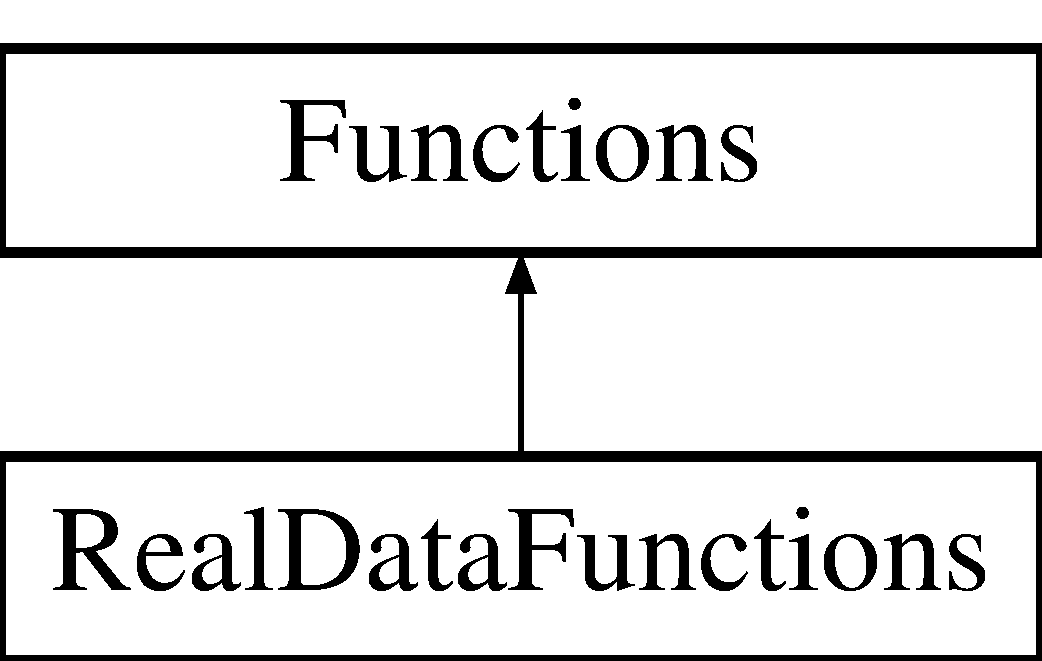
\includegraphics[height=2.000000cm]{class_real_data_functions}
\end{center}
\end{figure}
\subsection*{Public Member Functions}
\begin{DoxyCompactItemize}
\item 
\hyperlink{class_real_data_functions_a8c284fd674bf306d2069e984c7ea6c13}{Real\+Data\+Functions} (int d, int n, string file)
\item 
vector$<$ \hyperlink{class_multi_variate_point}{Multi\+Variate\+Point}$<$ double $>$ $>$ \hyperlink{class_real_data_functions_a9f25dd7676fe94730988fd244b71a158}{reference\+Pts} ()
\item 
vector$<$ vector$<$ double $>$ $>$ \hyperlink{class_real_data_functions_a0ff7f83b273d83d42053a1ce366d8637}{exact\+Values} ()
\item 
vector$<$ double $>$ \hyperlink{class_real_data_functions_a359a4965873b56bea2e19287b15ae585}{evaluate} (\hyperlink{class_multi_variate_point}{Multi\+Variate\+Point}$<$ double $>$ x)
\item 
void \hyperlink{class_real_data_functions_a84d811e14eca8b9f4d752cb1b3c700d9}{save\+Approximation\+Results} ()
\item 
void \hyperlink{class_real_data_functions_a0095f9185d37621decc568db26c7926c}{read\+Data\+From\+File} ()
\end{DoxyCompactItemize}
\subsection*{Additional Inherited Members}


\subsection{Constructor \& Destructor Documentation}
\index{Real\+Data\+Functions@{Real\+Data\+Functions}!Real\+Data\+Functions@{Real\+Data\+Functions}}
\index{Real\+Data\+Functions@{Real\+Data\+Functions}!Real\+Data\+Functions@{Real\+Data\+Functions}}
\subsubsection[{\texorpdfstring{Real\+Data\+Functions(int d, int n, string file)}{RealDataFunctions(int d, int n, string file)}}]{\setlength{\rightskip}{0pt plus 5cm}Real\+Data\+Functions\+::\+Real\+Data\+Functions (
\begin{DoxyParamCaption}
\item[{int}]{d, }
\item[{int}]{n, }
\item[{string}]{file}
\end{DoxyParamCaption}
)}\hypertarget{class_real_data_functions_a8c284fd674bf306d2069e984c7ea6c13}{}\label{class_real_data_functions_a8c284fd674bf306d2069e984c7ea6c13}
Constructeur 
\begin{DoxyParams}{Parameters}
{\em d} & dimension de l\textquotesingle{}éspace de départ de f \\
\hline
{\em n} & dimension de l\textquotesingle{}éspace de départ de f \\
\hline
{\em file} & nom du fichier de données \\
\hline
\end{DoxyParams}


\subsection{Member Function Documentation}
\index{Real\+Data\+Functions@{Real\+Data\+Functions}!evaluate@{evaluate}}
\index{evaluate@{evaluate}!Real\+Data\+Functions@{Real\+Data\+Functions}}
\subsubsection[{\texorpdfstring{evaluate(\+Multi\+Variate\+Point$<$ double $>$ x)}{evaluate(MultiVariatePoint< double > x)}}]{\setlength{\rightskip}{0pt plus 5cm}vector$<$double$>$ Real\+Data\+Functions\+::evaluate (
\begin{DoxyParamCaption}
\item[{{\bf Multi\+Variate\+Point}$<$ double $>$}]{x}
\end{DoxyParamCaption}
)\hspace{0.3cm}{\ttfamily [virtual]}}\hypertarget{class_real_data_functions_a359a4965873b56bea2e19287b15ae585}{}\label{class_real_data_functions_a359a4965873b56bea2e19287b15ae585}
Retourner la valeur \char`\"{}exacte\char`\"{} de f au point multivariée x 
\begin{DoxyParams}{Parameters}
{\em x} & \+: points multivarié \\
\hline
\end{DoxyParams}
\begin{DoxyReturn}{Returns}
f(x) \+: valeur de f au point x 
\end{DoxyReturn}


Implements \hyperlink{class_functions_a9d7bad8a6adacd8bd184a85a245e6168}{Functions}.

\index{Real\+Data\+Functions@{Real\+Data\+Functions}!exact\+Values@{exact\+Values}}
\index{exact\+Values@{exact\+Values}!Real\+Data\+Functions@{Real\+Data\+Functions}}
\subsubsection[{\texorpdfstring{exact\+Values()}{exactValues()}}]{\setlength{\rightskip}{0pt plus 5cm}vector$<$vector$<$double$>$ $>$ Real\+Data\+Functions\+::exact\+Values (
\begin{DoxyParamCaption}
{}
\end{DoxyParamCaption}
)\hspace{0.3cm}{\ttfamily [inline]}}\hypertarget{class_real_data_functions_a0ff7f83b273d83d42053a1ce366d8637}{}\label{class_real_data_functions_a0ff7f83b273d83d42053a1ce366d8637}
Retourner la liste des valeurs de f aux points de référence \begin{DoxyReturn}{Returns}
Ensemble des valeurs de f (peuvent être des valeurs vectorielles) 
\end{DoxyReturn}
\index{Real\+Data\+Functions@{Real\+Data\+Functions}!read\+Data\+From\+File@{read\+Data\+From\+File}}
\index{read\+Data\+From\+File@{read\+Data\+From\+File}!Real\+Data\+Functions@{Real\+Data\+Functions}}
\subsubsection[{\texorpdfstring{read\+Data\+From\+File()}{readDataFromFile()}}]{\setlength{\rightskip}{0pt plus 5cm}void Real\+Data\+Functions\+::read\+Data\+From\+File (
\begin{DoxyParamCaption}
{}
\end{DoxyParamCaption}
)}\hypertarget{class_real_data_functions_a0095f9185d37621decc568db26c7926c}{}\label{class_real_data_functions_a0095f9185d37621decc568db26c7926c}
Lire les données à partir du fichier m\+\_\+file\+Name et les stocker dans les attributs m\+\_\+reference\+Pts et m\+\_\+exact\+Values. Ils serviront à construire puis à évaluer l\textquotesingle{}opérateur d\textquotesingle{}interpolation. \index{Real\+Data\+Functions@{Real\+Data\+Functions}!reference\+Pts@{reference\+Pts}}
\index{reference\+Pts@{reference\+Pts}!Real\+Data\+Functions@{Real\+Data\+Functions}}
\subsubsection[{\texorpdfstring{reference\+Pts()}{referencePts()}}]{\setlength{\rightskip}{0pt plus 5cm}vector$<${\bf Multi\+Variate\+Point}$<$double$>$ $>$ Real\+Data\+Functions\+::reference\+Pts (
\begin{DoxyParamCaption}
{}
\end{DoxyParamCaption}
)\hspace{0.3cm}{\ttfamily [inline]}}\hypertarget{class_real_data_functions_a9f25dd7676fe94730988fd244b71a158}{}\label{class_real_data_functions_a9f25dd7676fe94730988fd244b71a158}
Retourner la liste des points de référence lus à partir du fichier m\+\_\+file\+Name \begin{DoxyReturn}{Returns}
Ensemble des points de références 
\end{DoxyReturn}
\index{Real\+Data\+Functions@{Real\+Data\+Functions}!save\+Approximation\+Results@{save\+Approximation\+Results}}
\index{save\+Approximation\+Results@{save\+Approximation\+Results}!Real\+Data\+Functions@{Real\+Data\+Functions}}
\subsubsection[{\texorpdfstring{save\+Approximation\+Results()}{saveApproximationResults()}}]{\setlength{\rightskip}{0pt plus 5cm}void Real\+Data\+Functions\+::save\+Approximation\+Results (
\begin{DoxyParamCaption}
{}
\end{DoxyParamCaption}
)}\hypertarget{class_real_data_functions_a84d811e14eca8b9f4d752cb1b3c700d9}{}\label{class_real_data_functions_a84d811e14eca8b9f4d752cb1b3c700d9}
Sauvegarder les résultats de l\textquotesingle{}interpolation dans le fichier output.\+data Ce fichier contient les mêmes infos présentes dans m\+\_\+file\+Name en plus des résultats de l\textquotesingle{}interolation adaptative ainsi que les erreurs d\textquotesingle{}interpolation (les 2 dernières colonnes séparées par $\vert$) 

The documentation for this class was generated from the following file\+:\begin{DoxyCompactItemize}
\item 
include/\hyperlink{_real_data_functions_8hpp}{Real\+Data\+Functions.\+hpp}\end{DoxyCompactItemize}

\hypertarget{class_utils}{}\section{Utils Class Reference}
\label{class_utils}\index{Utils@{Utils}}
\subsection*{Static Public Member Functions}
\begin{DoxyCompactItemize}
\item 
static void \hyperlink{class_utils_a02acfe9933a883a961f630cc60119daf}{display\+Values} (vector$<$ double $>$ v)
\item 
static double \hyperlink{class_utils_a3577821d384644fd163c2a83f47f03be}{min\+\_\+elt} (vector$<$ double $>$ v)
\item 
static double \hyperlink{class_utils_aa8f2a368c1da46a3798c45319958b67b}{max\+\_\+elt} (vector$<$ double $>$ v)
\item 
static double \hyperlink{class_utils_ab4db8a1cd94a91dd853c73696bb3ad67}{norm} (vector$<$ double $>$ x, int p)
\item 
static vector$<$ double $>$ \hyperlink{class_utils_ac229b7e4ffd41b36a272f35574e59a66}{diff} (vector$<$ double $>$ x, vector$<$ double $>$ y)
\item 
static double \hyperlink{class_utils_afac41428c306c6e26ce25831a94d2963}{convert\+To\+Default\+Domain} (double a, double b, double x)
\item 
static double \hyperlink{class_utils_a0e31da1f70e01bd5cc7b0edba2d38983}{convert\+To\+Function\+Domain} (double a, double b, double x)
\item 
static string \hyperlink{class_utils_a8a82a7ffe053f980c13d8dea64080ab9}{replace} (string strs, string str\+\_\+old, string str\+\_\+new)
\item 
static string \hyperlink{class_utils_a5014b4a0129213a5d596a0a287367d05}{erase\+Extra\+Spaces} (string strs)
\item 
static bool \hyperlink{class_utils_a088cf62d3a33c3f6836e9b6180a614be}{str\+In\+Vector} (string required, vector$<$ string $>$ vec)
\item 
static string \hyperlink{class_utils_a7a7b3dad14586624387060e0f7074b0c}{vector2str} (vector$<$ double $>$ x)
\item 
static vector$<$ double $>$ \hyperlink{class_utils_abac389cfb698e079e4674ccf1491720a}{str2vector} (string line)
\item 
static double \hyperlink{class_utils_ad3885d38d14f470daa040fb0abbad39f}{random\+Value} (double a, double b)
\item 
static \hyperlink{class_multi_variate_point}{Multi\+Variate\+Point}$<$ double $>$ \hyperlink{class_utils_a09a5b487abbd8c2233734aed6679a13a}{create\+Random\+Multi\+Variate\+Point} (int d)
\item 
static vector$<$ double $>$ \hyperlink{class_utils_aa03bde098ebd8a96a4a12b9581ea4721}{create\+Uniform\+Sequence} (int nb\+Points)
\item 
static vector$<$ double $>$ \hyperlink{class_utils_aa8b8ff1c9c1d271633aa9dd36990bd27}{create\+Chebychev\+Sequence} (int nb\+Points)
\item 
static vector$<$ double $>$ \hyperlink{class_utils_a829167caad4d105e52c1d4af4924a358}{create\+Leja\+Sequence} (int nb\+Points)
\item 
static vector$<$ double $>$ \hyperlink{class_utils_a13a74fc44a3300bc4053c92a98f9b55a}{load\+Leja\+Sequence\+From\+File} (int nb\+Points)
\item 
static void \hyperlink{class_utils_ace57ec8e6b8ac71fc13588c32f8e449e}{store\+Leja\+Sequence\+In\+File} (int nb\+Points)
\item 
static void \hyperlink{class_utils_a6ebd26c0dd01e720bcffc849c8a80e19}{binary\+Expansion} (int number, vector$<$ double $>$ \&binary\+\_\+decomp)
\item 
static bool \hyperlink{class_utils_aae5c071adea20e986aabc71119edb16f}{is\+Too\+Close\+To\+One\+Leja\+Point} (double y, vector$<$ double $>$ seq, double threshold)
\item 
static double \hyperlink{class_utils_a66a782d0cbfd519114e83c7be8139fea}{compute\+New\+Leja\+Point\+From\+Sequence} (vector$<$ double $>$ seq)
\item 
static bool \hyperlink{class_utils_ac7682da7749f473263a0f5dcdff946ce}{equals} (\hyperlink{class_multi_variate_point}{Multi\+Variate\+Point}$<$ string $>$ nu1, \hyperlink{class_multi_variate_point}{Multi\+Variate\+Point}$<$ string $>$ nu2)
\item 
static int \hyperlink{class_utils_ad56041abf23e7685a62bceef03a1042c}{choose\+DimensionD} (int argc, char $\ast$argv\mbox{[}$\,$\mbox{]}, int arg\+Num)
\item 
static int \hyperlink{class_utils_ac2699669d4b3c52444f3ac1ecb3252d4}{choose\+DimensionN} (int argc, char $\ast$argv\mbox{[}$\,$\mbox{]}, int arg\+Num)
\item 
static int \hyperlink{class_utils_a731fc80e8a40340da4dc1759fbd3f4cd}{choose\+Nb\+Test\+Points} (int argc, char $\ast$argv\mbox{[}$\,$\mbox{]}, int arg\+Num)
\item 
static int \hyperlink{class_utils_a030f2ded6b187b06a7f7994eb77a48a0}{choose\+Max\+Iteration} (int argc, char $\ast$argv\mbox{[}$\,$\mbox{]}, int arg\+Num)
\item 
static \hyperlink{class_multi_variate_point}{Multi\+Variate\+Point}$<$ int $>$ \hyperlink{class_utils_a42c046d922bf1427907e75ec027b175d}{choose\+Methods} (int dim)
\end{DoxyCompactItemize}
\subsection*{Static Public Attributes}
\begin{DoxyCompactItemize}
\item 
static double {\bfseries m\+\_\+precision}\hypertarget{class_utils_a844f2e98780e8237d94c0b6d676996fc}{}\label{class_utils_a844f2e98780e8237d94c0b6d676996fc}

\end{DoxyCompactItemize}


\subsection{Member Function Documentation}
\index{Utils@{Utils}!binary\+Expansion@{binary\+Expansion}}
\index{binary\+Expansion@{binary\+Expansion}!Utils@{Utils}}
\subsubsection[{\texorpdfstring{binary\+Expansion(int number, vector$<$ double $>$ \&binary\+\_\+decomp)}{binaryExpansion(int number, vector< double > &binary_decomp)}}]{\setlength{\rightskip}{0pt plus 5cm}static void Utils\+::binary\+Expansion (
\begin{DoxyParamCaption}
\item[{int}]{number, }
\item[{vector$<$ double $>$ \&}]{binary\+\_\+decomp}
\end{DoxyParamCaption}
)\hspace{0.3cm}{\ttfamily [static]}}\hypertarget{class_utils_a6ebd26c0dd01e720bcffc849c8a80e19}{}\label{class_utils_a6ebd26c0dd01e720bcffc849c8a80e19}
Calculer l\textquotesingle{}expansion binaire d\textquotesingle{}un entier number 
\begin{DoxyParams}{Parameters}
{\em number} & \+: Entier à décomposer \\
\hline
{\em binary\+\_\+decomp} & \+: expansion binaire de number sous forme de vecteur \\
\hline
\end{DoxyParams}
\index{Utils@{Utils}!choose\+DimensionD@{choose\+DimensionD}}
\index{choose\+DimensionD@{choose\+DimensionD}!Utils@{Utils}}
\subsubsection[{\texorpdfstring{choose\+Dimension\+D(int argc, char $\ast$argv[], int arg\+Num)}{chooseDimensionD(int argc, char *argv[], int argNum)}}]{\setlength{\rightskip}{0pt plus 5cm}static int Utils\+::choose\+DimensionD (
\begin{DoxyParamCaption}
\item[{int}]{argc, }
\item[{char $\ast$}]{argv\mbox{[}$\,$\mbox{]}, }
\item[{int}]{arg\+Num}
\end{DoxyParamCaption}
)\hspace{0.3cm}{\ttfamily [static]}}\hypertarget{class_utils_ad56041abf23e7685a62bceef03a1042c}{}\label{class_utils_ad56041abf23e7685a62bceef03a1042c}
Choisir la dimension d de l\textquotesingle{}espace de départ de f 
\begin{DoxyParams}{Parameters}
{\em argc} & \+: nombre d\textquotesingle{}arguments dans l\textquotesingle{}execution (arguments du main) \\
\hline
{\em argv} & \+: liste des arguments dans l\textquotesingle{}execution (arguments du main) \\
\hline
{\em arg\+Num} & \+: indice de l\textquotesingle{}argument concidéré \\
\hline
\end{DoxyParams}
\begin{DoxyReturn}{Returns}
dimension d 
\end{DoxyReturn}
\index{Utils@{Utils}!choose\+DimensionN@{choose\+DimensionN}}
\index{choose\+DimensionN@{choose\+DimensionN}!Utils@{Utils}}
\subsubsection[{\texorpdfstring{choose\+Dimension\+N(int argc, char $\ast$argv[], int arg\+Num)}{chooseDimensionN(int argc, char *argv[], int argNum)}}]{\setlength{\rightskip}{0pt plus 5cm}static int Utils\+::choose\+DimensionN (
\begin{DoxyParamCaption}
\item[{int}]{argc, }
\item[{char $\ast$}]{argv\mbox{[}$\,$\mbox{]}, }
\item[{int}]{arg\+Num}
\end{DoxyParamCaption}
)\hspace{0.3cm}{\ttfamily [static]}}\hypertarget{class_utils_ac2699669d4b3c52444f3ac1ecb3252d4}{}\label{class_utils_ac2699669d4b3c52444f3ac1ecb3252d4}
Choisir la dimension n de l\textquotesingle{}espace d\textquotesingle{}arrivé de f 
\begin{DoxyParams}{Parameters}
{\em argc} & \+: nombre d\textquotesingle{}arguments dans l\textquotesingle{}execution (arguments du main) \\
\hline
{\em argv} & \+: liste des arguments dans l\textquotesingle{}execution (arguments du main) \\
\hline
{\em arg\+Num} & \+: indice de l\textquotesingle{}argument concidéré \\
\hline
\end{DoxyParams}
\begin{DoxyReturn}{Returns}
dimension n 
\end{DoxyReturn}
\index{Utils@{Utils}!choose\+Max\+Iteration@{choose\+Max\+Iteration}}
\index{choose\+Max\+Iteration@{choose\+Max\+Iteration}!Utils@{Utils}}
\subsubsection[{\texorpdfstring{choose\+Max\+Iteration(int argc, char $\ast$argv[], int arg\+Num)}{chooseMaxIteration(int argc, char *argv[], int argNum)}}]{\setlength{\rightskip}{0pt plus 5cm}static int Utils\+::choose\+Max\+Iteration (
\begin{DoxyParamCaption}
\item[{int}]{argc, }
\item[{char $\ast$}]{argv\mbox{[}$\,$\mbox{]}, }
\item[{int}]{arg\+Num}
\end{DoxyParamCaption}
)\hspace{0.3cm}{\ttfamily [static]}}\hypertarget{class_utils_a030f2ded6b187b06a7f7994eb77a48a0}{}\label{class_utils_a030f2ded6b187b06a7f7994eb77a48a0}
Choisir le nombre d\textquotesingle{}itérations (ou nombre de points d\textquotesingle{}interpolation) dans l\textquotesingle{}algorithme AI 
\begin{DoxyParams}{Parameters}
{\em argc} & \+: nombre d\textquotesingle{}arguments dans l\textquotesingle{}execution (arguments du main) \\
\hline
{\em argv} & \+: liste des arguments dans l\textquotesingle{}execution (arguments du main) \\
\hline
{\em arg\+Num} & \+: indice de l\textquotesingle{}argument concidéré \\
\hline
\end{DoxyParams}
\begin{DoxyReturn}{Returns}
nombre d\textquotesingle{}itérations 
\end{DoxyReturn}
\index{Utils@{Utils}!choose\+Methods@{choose\+Methods}}
\index{choose\+Methods@{choose\+Methods}!Utils@{Utils}}
\subsubsection[{\texorpdfstring{choose\+Methods(int dim)}{chooseMethods(int dim)}}]{\setlength{\rightskip}{0pt plus 5cm}static {\bf Multi\+Variate\+Point}$<$int$>$ Utils\+::choose\+Methods (
\begin{DoxyParamCaption}
\item[{int}]{dim}
\end{DoxyParamCaption}
)\hspace{0.3cm}{\ttfamily [static]}}\hypertarget{class_utils_a42c046d922bf1427907e75ec027b175d}{}\label{class_utils_a42c046d922bf1427907e75ec027b175d}
Choisir la version de l\textquotesingle{}algorithme AI à utiliser dans chaque direction. Utile pour la version \hyperlink{class_mixed_interpolation}{Mixed\+Interpolation} 
\begin{DoxyParams}{Parameters}
{\em dim} & \+: dimension d de l\textquotesingle{}espace de depart de f \\
\hline
\end{DoxyParams}
\begin{DoxyReturn}{Returns}
multi-\/indice, chaque indice correspond à une version de AI 
\end{DoxyReturn}
\index{Utils@{Utils}!choose\+Nb\+Test\+Points@{choose\+Nb\+Test\+Points}}
\index{choose\+Nb\+Test\+Points@{choose\+Nb\+Test\+Points}!Utils@{Utils}}
\subsubsection[{\texorpdfstring{choose\+Nb\+Test\+Points(int argc, char $\ast$argv[], int arg\+Num)}{chooseNbTestPoints(int argc, char *argv[], int argNum)}}]{\setlength{\rightskip}{0pt plus 5cm}static int Utils\+::choose\+Nb\+Test\+Points (
\begin{DoxyParamCaption}
\item[{int}]{argc, }
\item[{char $\ast$}]{argv\mbox{[}$\,$\mbox{]}, }
\item[{int}]{arg\+Num}
\end{DoxyParamCaption}
)\hspace{0.3cm}{\ttfamily [static]}}\hypertarget{class_utils_a731fc80e8a40340da4dc1759fbd3f4cd}{}\label{class_utils_a731fc80e8a40340da4dc1759fbd3f4cd}
Choisir le nombre de points pour tester l\textquotesingle{}interpolant 
\begin{DoxyParams}{Parameters}
{\em argc} & \+: nombre d\textquotesingle{}arguments dans l\textquotesingle{}execution (arguments du main) \\
\hline
{\em argv} & \+: liste des arguments dans l\textquotesingle{}execution (arguments du main) \\
\hline
{\em arg\+Num} & \+: indice de l\textquotesingle{}argument concidéré \\
\hline
\end{DoxyParams}
\begin{DoxyReturn}{Returns}
nombre de points de test 
\end{DoxyReturn}
\index{Utils@{Utils}!compute\+New\+Leja\+Point\+From\+Sequence@{compute\+New\+Leja\+Point\+From\+Sequence}}
\index{compute\+New\+Leja\+Point\+From\+Sequence@{compute\+New\+Leja\+Point\+From\+Sequence}!Utils@{Utils}}
\subsubsection[{\texorpdfstring{compute\+New\+Leja\+Point\+From\+Sequence(vector$<$ double $>$ seq)}{computeNewLejaPointFromSequence(vector< double > seq)}}]{\setlength{\rightskip}{0pt plus 5cm}static double Utils\+::compute\+New\+Leja\+Point\+From\+Sequence (
\begin{DoxyParamCaption}
\item[{vector$<$ double $>$}]{seq}
\end{DoxyParamCaption}
)\hspace{0.3cm}{\ttfamily [static]}}\hypertarget{class_utils_a66a782d0cbfd519114e83c7be8139fea}{}\label{class_utils_a66a782d0cbfd519114e83c7be8139fea}
Calculer le nouveau point de Leja dans la liste de points seq 
\begin{DoxyParams}{Parameters}
{\em seq} & \+: sequence courante de Leja \\
\hline
\end{DoxyParams}
\begin{DoxyReturn}{Returns}
point de Leja suivant dans la sequence seq 
\end{DoxyReturn}
\index{Utils@{Utils}!convert\+To\+Default\+Domain@{convert\+To\+Default\+Domain}}
\index{convert\+To\+Default\+Domain@{convert\+To\+Default\+Domain}!Utils@{Utils}}
\subsubsection[{\texorpdfstring{convert\+To\+Default\+Domain(double a, double b, double x)}{convertToDefaultDomain(double a, double b, double x)}}]{\setlength{\rightskip}{0pt plus 5cm}static double Utils\+::convert\+To\+Default\+Domain (
\begin{DoxyParamCaption}
\item[{double}]{a, }
\item[{double}]{b, }
\item[{double}]{x}
\end{DoxyParamCaption}
)\hspace{0.3cm}{\ttfamily [static]}}\hypertarget{class_utils_afac41428c306c6e26ce25831a94d2963}{}\label{class_utils_afac41428c306c6e26ce25831a94d2963}
Changement de variable de \mbox{[}a,b\mbox{]} à \mbox{[}-\/1,1\mbox{]} 
\begin{DoxyParams}{Parameters}
{\em a} & \+: borne inf du ségment d\textquotesingle{}entrée \\
\hline
{\em b} & \+: borne sup du ségment d\textquotesingle{}entrée \\
\hline
{\em x} & \+: point à transformer \\
\hline
\end{DoxyParams}
\begin{DoxyReturn}{Returns}
x dans \mbox{[}-\/1,1\mbox{]} 
\end{DoxyReturn}
\index{Utils@{Utils}!convert\+To\+Function\+Domain@{convert\+To\+Function\+Domain}}
\index{convert\+To\+Function\+Domain@{convert\+To\+Function\+Domain}!Utils@{Utils}}
\subsubsection[{\texorpdfstring{convert\+To\+Function\+Domain(double a, double b, double x)}{convertToFunctionDomain(double a, double b, double x)}}]{\setlength{\rightskip}{0pt plus 5cm}static double Utils\+::convert\+To\+Function\+Domain (
\begin{DoxyParamCaption}
\item[{double}]{a, }
\item[{double}]{b, }
\item[{double}]{x}
\end{DoxyParamCaption}
)\hspace{0.3cm}{\ttfamily [static]}}\hypertarget{class_utils_a0e31da1f70e01bd5cc7b0edba2d38983}{}\label{class_utils_a0e31da1f70e01bd5cc7b0edba2d38983}
Changement de variable de \mbox{[}-\/1,1\mbox{]} à \mbox{[}a,b\mbox{]} 
\begin{DoxyParams}{Parameters}
{\em a} & \+: borne inf du ségment de sortie \\
\hline
{\em b} & \+: borne sup du ségment de sortie \\
\hline
{\em x} & \+: point à transformer \\
\hline
\end{DoxyParams}
\begin{DoxyReturn}{Returns}
x dans \mbox{[}a,b\mbox{]} 
\end{DoxyReturn}
\index{Utils@{Utils}!create\+Chebychev\+Sequence@{create\+Chebychev\+Sequence}}
\index{create\+Chebychev\+Sequence@{create\+Chebychev\+Sequence}!Utils@{Utils}}
\subsubsection[{\texorpdfstring{create\+Chebychev\+Sequence(int nb\+Points)}{createChebychevSequence(int nbPoints)}}]{\setlength{\rightskip}{0pt plus 5cm}static vector$<$double$>$ Utils\+::create\+Chebychev\+Sequence (
\begin{DoxyParamCaption}
\item[{int}]{nb\+Points}
\end{DoxyParamCaption}
)\hspace{0.3cm}{\ttfamily [static]}}\hypertarget{class_utils_aa8b8ff1c9c1d271633aa9dd36990bd27}{}\label{class_utils_aa8b8ff1c9c1d271633aa9dd36990bd27}
Créer la sequence de Chebychev de nb\+Points points 1d 
\begin{DoxyParams}{Parameters}
{\em nb\+Points} & \+: taille de la séquence \\
\hline
\end{DoxyParams}
\begin{DoxyReturn}{Returns}
séquence de Chebychev 
\end{DoxyReturn}
\index{Utils@{Utils}!create\+Leja\+Sequence@{create\+Leja\+Sequence}}
\index{create\+Leja\+Sequence@{create\+Leja\+Sequence}!Utils@{Utils}}
\subsubsection[{\texorpdfstring{create\+Leja\+Sequence(int nb\+Points)}{createLejaSequence(int nbPoints)}}]{\setlength{\rightskip}{0pt plus 5cm}static vector$<$double$>$ Utils\+::create\+Leja\+Sequence (
\begin{DoxyParamCaption}
\item[{int}]{nb\+Points}
\end{DoxyParamCaption}
)\hspace{0.3cm}{\ttfamily [static]}}\hypertarget{class_utils_a829167caad4d105e52c1d4af4924a358}{}\label{class_utils_a829167caad4d105e52c1d4af4924a358}
Créer la sequence de Leja de nb\+Points points 1d 
\begin{DoxyParams}{Parameters}
{\em nb\+Points} & \+: taille de la séquence \\
\hline
\end{DoxyParams}
\begin{DoxyReturn}{Returns}
séquence de Leja 
\end{DoxyReturn}
\index{Utils@{Utils}!create\+Random\+Multi\+Variate\+Point@{create\+Random\+Multi\+Variate\+Point}}
\index{create\+Random\+Multi\+Variate\+Point@{create\+Random\+Multi\+Variate\+Point}!Utils@{Utils}}
\subsubsection[{\texorpdfstring{create\+Random\+Multi\+Variate\+Point(int d)}{createRandomMultiVariatePoint(int d)}}]{\setlength{\rightskip}{0pt plus 5cm}static {\bf Multi\+Variate\+Point}$<$double$>$ Utils\+::create\+Random\+Multi\+Variate\+Point (
\begin{DoxyParamCaption}
\item[{int}]{d}
\end{DoxyParamCaption}
)\hspace{0.3cm}{\ttfamily [static]}}\hypertarget{class_utils_a09a5b487abbd8c2233734aed6679a13a}{}\label{class_utils_a09a5b487abbd8c2233734aed6679a13a}
Retourner un point multivarié dans \mbox{[}-\/1,1\mbox{]}$^\wedge$d d\textquotesingle{}une manière aléatoire 
\begin{DoxyParams}{Parameters}
{\em d} & \+: taille du point \\
\hline
\end{DoxyParams}
\begin{DoxyReturn}{Returns}
point multivarié aléatoire 
\end{DoxyReturn}
\index{Utils@{Utils}!create\+Uniform\+Sequence@{create\+Uniform\+Sequence}}
\index{create\+Uniform\+Sequence@{create\+Uniform\+Sequence}!Utils@{Utils}}
\subsubsection[{\texorpdfstring{create\+Uniform\+Sequence(int nb\+Points)}{createUniformSequence(int nbPoints)}}]{\setlength{\rightskip}{0pt plus 5cm}static vector$<$double$>$ Utils\+::create\+Uniform\+Sequence (
\begin{DoxyParamCaption}
\item[{int}]{nb\+Points}
\end{DoxyParamCaption}
)\hspace{0.3cm}{\ttfamily [static]}}\hypertarget{class_utils_aa03bde098ebd8a96a4a12b9581ea4721}{}\label{class_utils_aa03bde098ebd8a96a4a12b9581ea4721}
Créer une sequence uniforme de nb\+Points points 1d dans \mbox{[}-\/1,1\mbox{]} 
\begin{DoxyParams}{Parameters}
{\em nb\+Points} & \+: taille de la séquence \\
\hline
\end{DoxyParams}
\begin{DoxyReturn}{Returns}
séquence uniforme de points 
\end{DoxyReturn}
\index{Utils@{Utils}!diff@{diff}}
\index{diff@{diff}!Utils@{Utils}}
\subsubsection[{\texorpdfstring{diff(vector$<$ double $>$ x, vector$<$ double $>$ y)}{diff(vector< double > x, vector< double > y)}}]{\setlength{\rightskip}{0pt plus 5cm}static vector$<$double$>$ Utils\+::diff (
\begin{DoxyParamCaption}
\item[{vector$<$ double $>$}]{x, }
\item[{vector$<$ double $>$}]{y}
\end{DoxyParamCaption}
)\hspace{0.3cm}{\ttfamily [static]}}\hypertarget{class_utils_ac229b7e4ffd41b36a272f35574e59a66}{}\label{class_utils_ac229b7e4ffd41b36a272f35574e59a66}
Calculer la difference entre 2 vecteurs x et y 
\begin{DoxyParams}{Parameters}
{\em x} & \+: vecteur de double \\
\hline
{\em y} & \+: vecteur de double \\
\hline
\end{DoxyParams}
\begin{DoxyReturn}{Returns}
x -\/ y = (x\+\_\+i -\/ y\+\_\+i)\+\_\+i 
\end{DoxyReturn}
\index{Utils@{Utils}!display\+Values@{display\+Values}}
\index{display\+Values@{display\+Values}!Utils@{Utils}}
\subsubsection[{\texorpdfstring{display\+Values(vector$<$ double $>$ v)}{displayValues(vector< double > v)}}]{\setlength{\rightskip}{0pt plus 5cm}static void Utils\+::display\+Values (
\begin{DoxyParamCaption}
\item[{vector$<$ double $>$}]{v}
\end{DoxyParamCaption}
)\hspace{0.3cm}{\ttfamily [static]}}\hypertarget{class_utils_a02acfe9933a883a961f630cc60119daf}{}\label{class_utils_a02acfe9933a883a961f630cc60119daf}
Fonction pour afficher les élément d\textquotesingle{}un vecteur 
\begin{DoxyParams}{Parameters}
{\em v} & \+: vecteur à afficher \\
\hline
\end{DoxyParams}
\index{Utils@{Utils}!equals@{equals}}
\index{equals@{equals}!Utils@{Utils}}
\subsubsection[{\texorpdfstring{equals(\+Multi\+Variate\+Point$<$ string $>$ nu1, Multi\+Variate\+Point$<$ string $>$ nu2)}{equals(MultiVariatePoint< string > nu1, MultiVariatePoint< string > nu2)}}]{\setlength{\rightskip}{0pt plus 5cm}static bool Utils\+::equals (
\begin{DoxyParamCaption}
\item[{{\bf Multi\+Variate\+Point}$<$ string $>$}]{nu1, }
\item[{{\bf Multi\+Variate\+Point}$<$ string $>$}]{nu2}
\end{DoxyParamCaption}
)\hspace{0.3cm}{\ttfamily [static]}}\hypertarget{class_utils_ac7682da7749f473263a0f5dcdff946ce}{}\label{class_utils_ac7682da7749f473263a0f5dcdff946ce}
Test d\textquotesingle{}égalité entre les points multivariés nu1 et nu2 
\begin{DoxyParams}{Parameters}
{\em nu1} & \+: point multivarié \\
\hline
{\em nu2} & \+: point multivarié \\
\hline
\end{DoxyParams}
\begin{DoxyReturn}{Returns}
True si et seulement si nu1 = nu2 
\end{DoxyReturn}
\index{Utils@{Utils}!erase\+Extra\+Spaces@{erase\+Extra\+Spaces}}
\index{erase\+Extra\+Spaces@{erase\+Extra\+Spaces}!Utils@{Utils}}
\subsubsection[{\texorpdfstring{erase\+Extra\+Spaces(string strs)}{eraseExtraSpaces(string strs)}}]{\setlength{\rightskip}{0pt plus 5cm}static string Utils\+::erase\+Extra\+Spaces (
\begin{DoxyParamCaption}
\item[{string}]{strs}
\end{DoxyParamCaption}
)\hspace{0.3cm}{\ttfamily [static]}}\hypertarget{class_utils_a5014b4a0129213a5d596a0a287367d05}{}\label{class_utils_a5014b4a0129213a5d596a0a287367d05}
Supprimer les espaces de séparation inutiles dans strs En sortie strs est une chaine de caractères contenant des réels séparés par un seul espace 
\begin{DoxyParams}{Parameters}
{\em strs} & \+: chaine de caractère \\
\hline
\end{DoxyParams}
\begin{DoxyReturn}{Returns}
strs sans espaces inutiles 
\end{DoxyReturn}
\index{Utils@{Utils}!is\+Too\+Close\+To\+One\+Leja\+Point@{is\+Too\+Close\+To\+One\+Leja\+Point}}
\index{is\+Too\+Close\+To\+One\+Leja\+Point@{is\+Too\+Close\+To\+One\+Leja\+Point}!Utils@{Utils}}
\subsubsection[{\texorpdfstring{is\+Too\+Close\+To\+One\+Leja\+Point(double y, vector$<$ double $>$ seq, double threshold)}{isTooCloseToOneLejaPoint(double y, vector< double > seq, double threshold)}}]{\setlength{\rightskip}{0pt plus 5cm}static bool Utils\+::is\+Too\+Close\+To\+One\+Leja\+Point (
\begin{DoxyParamCaption}
\item[{double}]{y, }
\item[{vector$<$ double $>$}]{seq, }
\item[{double}]{threshold}
\end{DoxyParamCaption}
)\hspace{0.3cm}{\ttfamily [static]}}\hypertarget{class_utils_aae5c071adea20e986aabc71119edb16f}{}\label{class_utils_aae5c071adea20e986aabc71119edb16f}
Verifier si le point y est trés proche d\textquotesingle{}un point de la séquence seq 
\begin{DoxyParams}{Parameters}
{\em y} & \+: point concidéré \\
\hline
{\em seq} & \+: sequence de points 1d \\
\hline
{\em threshold} & \+: seuil de comparaison \\
\hline
\end{DoxyParams}
\begin{DoxyReturn}{Returns}
True si la distance de y à un point de seq est inférieure à threshold 
\end{DoxyReturn}
\index{Utils@{Utils}!load\+Leja\+Sequence\+From\+File@{load\+Leja\+Sequence\+From\+File}}
\index{load\+Leja\+Sequence\+From\+File@{load\+Leja\+Sequence\+From\+File}!Utils@{Utils}}
\subsubsection[{\texorpdfstring{load\+Leja\+Sequence\+From\+File(int nb\+Points)}{loadLejaSequenceFromFile(int nbPoints)}}]{\setlength{\rightskip}{0pt plus 5cm}static vector$<$double$>$ Utils\+::load\+Leja\+Sequence\+From\+File (
\begin{DoxyParamCaption}
\item[{int}]{nb\+Points}
\end{DoxyParamCaption}
)\hspace{0.3cm}{\ttfamily [static]}}\hypertarget{class_utils_a13a74fc44a3300bc4053c92a98f9b55a}{}\label{class_utils_a13a74fc44a3300bc4053c92a98f9b55a}
Charger la sequence de Leja de nb\+Points points 1d depuis le fichier data/leja\+\_\+sequence.\+dat 
\begin{DoxyParams}{Parameters}
{\em nb\+Points} & \+: taille de la séquence \\
\hline
\end{DoxyParams}
\begin{DoxyReturn}{Returns}
séquence de Leja 
\end{DoxyReturn}
\index{Utils@{Utils}!max\+\_\+elt@{max\+\_\+elt}}
\index{max\+\_\+elt@{max\+\_\+elt}!Utils@{Utils}}
\subsubsection[{\texorpdfstring{max\+\_\+elt(vector$<$ double $>$ v)}{max_elt(vector< double > v)}}]{\setlength{\rightskip}{0pt plus 5cm}static double Utils\+::max\+\_\+elt (
\begin{DoxyParamCaption}
\item[{vector$<$ double $>$}]{v}
\end{DoxyParamCaption}
)\hspace{0.3cm}{\ttfamily [static]}}\hypertarget{class_utils_aa8f2a368c1da46a3798c45319958b67b}{}\label{class_utils_aa8f2a368c1da46a3798c45319958b67b}
Chercher le max d\textquotesingle{}un vecteur 
\begin{DoxyParams}{Parameters}
{\em v} & \+: vecteur de double \\
\hline
\end{DoxyParams}
\begin{DoxyReturn}{Returns}
element max de v 
\end{DoxyReturn}
\index{Utils@{Utils}!min\+\_\+elt@{min\+\_\+elt}}
\index{min\+\_\+elt@{min\+\_\+elt}!Utils@{Utils}}
\subsubsection[{\texorpdfstring{min\+\_\+elt(vector$<$ double $>$ v)}{min_elt(vector< double > v)}}]{\setlength{\rightskip}{0pt plus 5cm}static double Utils\+::min\+\_\+elt (
\begin{DoxyParamCaption}
\item[{vector$<$ double $>$}]{v}
\end{DoxyParamCaption}
)\hspace{0.3cm}{\ttfamily [static]}}\hypertarget{class_utils_a3577821d384644fd163c2a83f47f03be}{}\label{class_utils_a3577821d384644fd163c2a83f47f03be}
Chercher le mix d\textquotesingle{}un vecteur 
\begin{DoxyParams}{Parameters}
{\em v} & \+: vecteur de double \\
\hline
\end{DoxyParams}
\begin{DoxyReturn}{Returns}
element min de v 
\end{DoxyReturn}
\index{Utils@{Utils}!norm@{norm}}
\index{norm@{norm}!Utils@{Utils}}
\subsubsection[{\texorpdfstring{norm(vector$<$ double $>$ x, int p)}{norm(vector< double > x, int p)}}]{\setlength{\rightskip}{0pt plus 5cm}static double Utils\+::norm (
\begin{DoxyParamCaption}
\item[{vector$<$ double $>$}]{x, }
\item[{int}]{p}
\end{DoxyParamCaption}
)\hspace{0.3cm}{\ttfamily [static]}}\hypertarget{class_utils_ab4db8a1cd94a91dd853c73696bb3ad67}{}\label{class_utils_ab4db8a1cd94a91dd853c73696bb3ad67}
Calculer la norme d\textquotesingle{}un vecteur v si p = 0 --$>$ norme infini si p != 0 --$>$ norme 2 
\begin{DoxyParams}{Parameters}
{\em v} & \+: vecteur de double \\
\hline
\end{DoxyParams}
\begin{DoxyReturn}{Returns}
norme de x 
\end{DoxyReturn}
\index{Utils@{Utils}!random\+Value@{random\+Value}}
\index{random\+Value@{random\+Value}!Utils@{Utils}}
\subsubsection[{\texorpdfstring{random\+Value(double a, double b)}{randomValue(double a, double b)}}]{\setlength{\rightskip}{0pt plus 5cm}static double Utils\+::random\+Value (
\begin{DoxyParamCaption}
\item[{double}]{a, }
\item[{double}]{b}
\end{DoxyParamCaption}
)\hspace{0.3cm}{\ttfamily [static]}}\hypertarget{class_utils_ad3885d38d14f470daa040fb0abbad39f}{}\label{class_utils_ad3885d38d14f470daa040fb0abbad39f}
Retourner une valeur entre a et b aléatoirement 
\begin{DoxyParams}{Parameters}
{\em a} & \+: borne inf \\
\hline
{\em b} & \+: borne sup \\
\hline
\end{DoxyParams}
\begin{DoxyReturn}{Returns}
valeur entre a et b 
\end{DoxyReturn}
\index{Utils@{Utils}!replace@{replace}}
\index{replace@{replace}!Utils@{Utils}}
\subsubsection[{\texorpdfstring{replace(string strs, string str\+\_\+old, string str\+\_\+new)}{replace(string strs, string str_old, string str_new)}}]{\setlength{\rightskip}{0pt plus 5cm}static string Utils\+::replace (
\begin{DoxyParamCaption}
\item[{string}]{strs, }
\item[{string}]{str\+\_\+old, }
\item[{string}]{str\+\_\+new}
\end{DoxyParamCaption}
)\hspace{0.3cm}{\ttfamily [static]}}\hypertarget{class_utils_a8a82a7ffe053f980c13d8dea64080ab9}{}\label{class_utils_a8a82a7ffe053f980c13d8dea64080ab9}
Remplacer dans strs les sous-\/chaines str\+\_\+old par str\+\_\+new 
\begin{DoxyParams}{Parameters}
{\em strs} & \+: chaine de caractère \\
\hline
{\em str\+\_\+old} & \+: sous-\/chaine remplacé \\
\hline
{\em new\+\_\+old} & \+: nouvelle sous-\/chaine \\
\hline
\end{DoxyParams}
\begin{DoxyReturn}{Returns}
nouveau strs 
\end{DoxyReturn}
\index{Utils@{Utils}!store\+Leja\+Sequence\+In\+File@{store\+Leja\+Sequence\+In\+File}}
\index{store\+Leja\+Sequence\+In\+File@{store\+Leja\+Sequence\+In\+File}!Utils@{Utils}}
\subsubsection[{\texorpdfstring{store\+Leja\+Sequence\+In\+File(int nb\+Points)}{storeLejaSequenceInFile(int nbPoints)}}]{\setlength{\rightskip}{0pt plus 5cm}static void Utils\+::store\+Leja\+Sequence\+In\+File (
\begin{DoxyParamCaption}
\item[{int}]{nb\+Points}
\end{DoxyParamCaption}
)\hspace{0.3cm}{\ttfamily [static]}}\hypertarget{class_utils_ace57ec8e6b8ac71fc13588c32f8e449e}{}\label{class_utils_ace57ec8e6b8ac71fc13588c32f8e449e}
Créer puis sauvegarder dans le fichier data/leja\+\_\+sequence.\+dat la sequence de Leja de nb\+Points points 1d 
\begin{DoxyParams}{Parameters}
{\em nb\+Points} & \+: taille de la séquence \\
\hline
\end{DoxyParams}
\index{Utils@{Utils}!str2vector@{str2vector}}
\index{str2vector@{str2vector}!Utils@{Utils}}
\subsubsection[{\texorpdfstring{str2vector(string line)}{str2vector(string line)}}]{\setlength{\rightskip}{0pt plus 5cm}static vector$<$double$>$ Utils\+::str2vector (
\begin{DoxyParamCaption}
\item[{string}]{line}
\end{DoxyParamCaption}
)\hspace{0.3cm}{\ttfamily [static]}}\hypertarget{class_utils_abac389cfb698e079e4674ccf1491720a}{}\label{class_utils_abac389cfb698e079e4674ccf1491720a}
Transformer la chaine de caractère line en vecteur de double 
\begin{DoxyParams}{Parameters}
{\em line} & \+: chaine de caractere à transformer \\
\hline
\end{DoxyParams}
\begin{DoxyReturn}{Returns}
vecteur de double 
\end{DoxyReturn}
\index{Utils@{Utils}!str\+In\+Vector@{str\+In\+Vector}}
\index{str\+In\+Vector@{str\+In\+Vector}!Utils@{Utils}}
\subsubsection[{\texorpdfstring{str\+In\+Vector(string required, vector$<$ string $>$ vec)}{strInVector(string required, vector< string > vec)}}]{\setlength{\rightskip}{0pt plus 5cm}static bool Utils\+::str\+In\+Vector (
\begin{DoxyParamCaption}
\item[{string}]{required, }
\item[{vector$<$ string $>$}]{vec}
\end{DoxyParamCaption}
)\hspace{0.3cm}{\ttfamily [static]}}\hypertarget{class_utils_a088cf62d3a33c3f6836e9b6180a614be}{}\label{class_utils_a088cf62d3a33c3f6836e9b6180a614be}
Vérifier si la chaine required existe dans le vecteur de chaine vec 
\begin{DoxyParams}{Parameters}
{\em required} & \+: chaine de caractère recherchée \\
\hline
{\em vec} & \+: vecteur de chaines de caractère \\
\hline
\end{DoxyParams}
\begin{DoxyReturn}{Returns}
True si et seulement si requirede st un element de vec 
\end{DoxyReturn}
\index{Utils@{Utils}!vector2str@{vector2str}}
\index{vector2str@{vector2str}!Utils@{Utils}}
\subsubsection[{\texorpdfstring{vector2str(vector$<$ double $>$ x)}{vector2str(vector< double > x)}}]{\setlength{\rightskip}{0pt plus 5cm}static string Utils\+::vector2str (
\begin{DoxyParamCaption}
\item[{vector$<$ double $>$}]{x}
\end{DoxyParamCaption}
)\hspace{0.3cm}{\ttfamily [static]}}\hypertarget{class_utils_a7a7b3dad14586624387060e0f7074b0c}{}\label{class_utils_a7a7b3dad14586624387060e0f7074b0c}
Transformer le vecteur x en chaine de caractère en séparant les double par un espace 
\begin{DoxyParams}{Parameters}
{\em x} & \+: vecteur de double \\
\hline
\end{DoxyParams}
\begin{DoxyReturn}{Returns}
x sous forme de chaine de caractere 
\end{DoxyReturn}


The documentation for this class was generated from the following file\+:\begin{DoxyCompactItemize}
\item 
A\+I/include/\hyperlink{_utils_8hpp}{Utils.\+hpp}\end{DoxyCompactItemize}

\chapter{File Documentation}
\hypertarget{_analytical_functions_8hpp}{}\section{include/\+Analytical\+Functions.hpp File Reference}
\label{_analytical_functions_8hpp}\index{include/\+Analytical\+Functions.\+hpp@{include/\+Analytical\+Functions.\+hpp}}


Classe dérivée de \hyperlink{class_functions}{Functions}\+: implémente des exemples de fonctions analytiques. Permet de valider la méthode.  


{\ttfamily \#include $<$fstream$>$}\\*
{\ttfamily \#include $<$iostream$>$}\\*
{\ttfamily \#include $<$vector$>$}\\*
{\ttfamily \#include $<$string$>$}\\*
{\ttfamily \#include $<$sstream$>$}\\*
{\ttfamily \#include $<$cmath$>$}\\*
{\ttfamily \#include $<$limits$>$}\\*
{\ttfamily \#include $<$stdio.\+h$>$}\\*
{\ttfamily \#include \char`\"{}Multi\+Variate\+Point.\+hpp\char`\"{}}\\*
{\ttfamily \#include \char`\"{}Functions.\+hpp\char`\"{}}\\*
\subsection*{Classes}
\begin{DoxyCompactItemize}
\item 
class \hyperlink{class_analytical_functions}{Analytical\+Functions}
\end{DoxyCompactItemize}
\subsection*{Typedefs}
\begin{DoxyCompactItemize}
\item 
typedef std\+::shared\+\_\+ptr$<$ \hyperlink{class_analytical_functions}{Analytical\+Functions} $>$ {\bfseries Analytical\+Functions\+Ptr}\hypertarget{_analytical_functions_8hpp_aa55d0b01c6cf06c9717896e999d15d60}{}\label{_analytical_functions_8hpp_aa55d0b01c6cf06c9717896e999d15d60}

\end{DoxyCompactItemize}


\subsection{Detailed Description}
Classe dérivée de \hyperlink{class_functions}{Functions}\+: implémente des exemples de fonctions analytiques. Permet de valider la méthode. 

\begin{DoxyAuthor}{Author}
S\+I\+A\+LA Rafik 
\end{DoxyAuthor}
\begin{DoxyDate}{Date}
08/16 
\end{DoxyDate}

\hypertarget{_binary_tree_8hpp}{}\section{include/\+Binary\+Tree.hpp File Reference}
\label{_binary_tree_8hpp}\index{include/\+Binary\+Tree.\+hpp@{include/\+Binary\+Tree.\+hpp}}


Classe qui implémente un arbre binaire de recherche. Utile pour la version \hyperlink{class_piecewise_interpolation}{Piecewise\+Interpolation}.  


{\ttfamily \#include $<$fstream$>$}\\*
{\ttfamily \#include $<$iostream$>$}\\*
{\ttfamily \#include $<$vector$>$}\\*
{\ttfamily \#include $<$string$>$}\\*
{\ttfamily \#include $<$map$>$}\\*
{\ttfamily \#include $<$algorithm$>$}\\*
{\ttfamily \#include $<$cstring$>$}\\*
{\ttfamily \#include $<$memory$>$}\\*
{\ttfamily \#include $<$limits$>$}\\*
{\ttfamily \#include $<$iomanip$>$}\\*
\subsection*{Classes}
\begin{DoxyCompactItemize}
\item 
class \hyperlink{class_node}{Node}
\item 
class \hyperlink{class_binary_tree}{Binary\+Tree}
\end{DoxyCompactItemize}
\subsection*{Typedefs}
\begin{DoxyCompactItemize}
\item 
typedef std\+::shared\+\_\+ptr$<$ \hyperlink{class_binary_tree}{Binary\+Tree} $>$ {\bfseries Binary\+Tree\+Ptr}\hypertarget{_binary_tree_8hpp_ac569688f580c3d07e2c425c8f29a1818}{}\label{_binary_tree_8hpp_ac569688f580c3d07e2c425c8f29a1818}

\end{DoxyCompactItemize}


\subsection{Detailed Description}
Classe qui implémente un arbre binaire de recherche. Utile pour la version \hyperlink{class_piecewise_interpolation}{Piecewise\+Interpolation}. 

\begin{DoxyAuthor}{Author}
S\+I\+A\+LA Rafik 
\end{DoxyAuthor}
\begin{DoxyDate}{Date}
08/16 
\end{DoxyDate}

\hypertarget{_functions_8hpp}{}\section{A\+I/include/\+Functions.hpp File Reference}
\label{_functions_8hpp}\index{A\+I/include/\+Functions.\+hpp@{A\+I/include/\+Functions.\+hpp}}


Classe de base abstraite modélisant les diffèrents types de fonctions qu\textquotesingle{}on veut approcher (fonctions analytiques ou données réelles)  


{\ttfamily \#include $<$fstream$>$}\\*
{\ttfamily \#include $<$iostream$>$}\\*
{\ttfamily \#include $<$vector$>$}\\*
{\ttfamily \#include $<$string$>$}\\*
{\ttfamily \#include $<$sstream$>$}\\*
{\ttfamily \#include $<$cmath$>$}\\*
{\ttfamily \#include $<$limits$>$}\\*
{\ttfamily \#include $<$stdio.\+h$>$}\\*
{\ttfamily \#include \char`\"{}Multi\+Variate\+Point.\+hpp\char`\"{}}\\*
{\ttfamily \#include \char`\"{}Utils.\+hpp\char`\"{}}\\*
Include dependency graph for Functions.\+hpp\+:
% FIG 0
This graph shows which files directly or indirectly include this file\+:
% FIG 1
\subsection*{Classes}
\begin{DoxyCompactItemize}
\item 
class \hyperlink{class_functions}{Functions}
\end{DoxyCompactItemize}
\subsection*{Macros}
\begin{DoxyCompactItemize}
\item 
\#define {\bfseries B\+U\+F\+S\+I\+ZE}~1024\hypertarget{_functions_8hpp_aeca034f67218340ecb2261a22c2f3dcd}{}\label{_functions_8hpp_aeca034f67218340ecb2261a22c2f3dcd}

\end{DoxyCompactItemize}
\subsection*{Typedefs}
\begin{DoxyCompactItemize}
\item 
typedef std\+::shared\+\_\+ptr$<$ \hyperlink{class_functions}{Functions} $>$ {\bfseries Functions\+Ptr}\hypertarget{_functions_8hpp_a6eaaa7cd355623de484ea75f1ef039b3}{}\label{_functions_8hpp_a6eaaa7cd355623de484ea75f1ef039b3}

\end{DoxyCompactItemize}


\subsection{Detailed Description}
Classe de base abstraite modélisant les diffèrents types de fonctions qu\textquotesingle{}on veut approcher (fonctions analytiques ou données réelles) 

\begin{DoxyAuthor}{Author}
S\+I\+A\+LA Rafik 
\end{DoxyAuthor}
\begin{DoxyDate}{Date}
08/16 
\end{DoxyDate}

\hypertarget{_interpolation_8hpp}{}\section{include/\+Interpolation.hpp File Reference}
\label{_interpolation_8hpp}\index{include/\+Interpolation.\+hpp@{include/\+Interpolation.\+hpp}}


Classe générique abstraite qui implémente l\textquotesingle{}algorithme d\textquotesingle{}interpolation adaptative.  


{\ttfamily \#include $<$iostream$>$}\\*
{\ttfamily \#include $<$vector$>$}\\*
{\ttfamily \#include $<$list$>$}\\*
{\ttfamily \#include $<$set$>$}\\*
{\ttfamily \#include $<$map$>$}\\*
{\ttfamily \#include $<$memory$>$}\\*
{\ttfamily \#include $<$cmath$>$}\\*
{\ttfamily \#include $<$chrono$>$}\\*
{\ttfamily \#include $<$iomanip$>$}\\*
{\ttfamily \#include $<$limits$>$}\\*
{\ttfamily \#include \char`\"{}Multi\+Variate\+Point.\+hpp\char`\"{}}\\*
{\ttfamily \#include \char`\"{}Binary\+Tree.\+hpp\char`\"{}}\\*
{\ttfamily \#include \char`\"{}Functions.\+hpp\char`\"{}}\\*
{\ttfamily \#include \char`\"{}Utils.\+hpp\char`\"{}}\\*
\subsection*{Classes}
\begin{DoxyCompactItemize}
\item 
class \hyperlink{class_interpolation}{Interpolation$<$ T $>$}
\end{DoxyCompactItemize}
\subsection*{Typedefs}
\begin{DoxyCompactItemize}
\item 
{\footnotesize template$<$typename T $>$ }\\using {\bfseries Interpolation\+Ptr} = shared\+\_\+ptr$<$ \hyperlink{class_interpolation}{Interpolation}$<$ T $>$$>$\hypertarget{_interpolation_8hpp_a9422e675c72b83cc1a07fb8bd4a48092}{}\label{_interpolation_8hpp_a9422e675c72b83cc1a07fb8bd4a48092}

\end{DoxyCompactItemize}


\subsection{Detailed Description}
Classe générique abstraite qui implémente l\textquotesingle{}algorithme d\textquotesingle{}interpolation adaptative. 

\begin{DoxyAuthor}{Author}
S\+I\+A\+LA Rafik 
\end{DoxyAuthor}
\begin{DoxyDate}{Date}
08/16 
\end{DoxyDate}

\hypertarget{_lagrange_interpolation_8hpp}{}\section{A\+I/include/\+Lagrange\+Interpolation.hpp File Reference}
\label{_lagrange_interpolation_8hpp}\index{A\+I/include/\+Lagrange\+Interpolation.\+hpp@{A\+I/include/\+Lagrange\+Interpolation.\+hpp}}


Classe dérivée de \hyperlink{class_interpolation}{Interpolation$<$int$>$}\+: interpolation utilisant des polynomes de Lagrange définis globalement et les points de Leja. Le type d\textquotesingle{}ordre est un entier (multindice en grande dimension) correspond à l\textquotesingle{}indice du point dans la séquence de Leja.  


{\ttfamily \#include $<$iostream$>$}\\*
{\ttfamily \#include $<$vector$>$}\\*
{\ttfamily \#include $<$list$>$}\\*
{\ttfamily \#include $<$map$>$}\\*
{\ttfamily \#include $<$memory$>$}\\*
{\ttfamily \#include $<$cmath$>$}\\*
{\ttfamily \#include $<$chrono$>$}\\*
{\ttfamily \#include \char`\"{}Multi\+Variate\+Point.\+hpp\char`\"{}}\\*
{\ttfamily \#include \char`\"{}Interpolation.\+hpp\char`\"{}}\\*
{\ttfamily \#include \char`\"{}Binary\+Tree.\+hpp\char`\"{}}\\*
{\ttfamily \#include \char`\"{}Utils.\+hpp\char`\"{}}\\*
Include dependency graph for Lagrange\+Interpolation.\+hpp\+:
% FIG 0
\subsection*{Classes}
\begin{DoxyCompactItemize}
\item 
class \hyperlink{class_lagrange_interpolation}{Lagrange\+Interpolation}
\end{DoxyCompactItemize}
\subsection*{Typedefs}
\begin{DoxyCompactItemize}
\item 
typedef std\+::unique\+\_\+ptr$<$ \hyperlink{class_lagrange_interpolation}{Lagrange\+Interpolation} $>$ {\bfseries Lagrange\+Interpolation\+Ptr}\hypertarget{_lagrange_interpolation_8hpp_a06bd30da2f1fafffd4c4472db51408b3}{}\label{_lagrange_interpolation_8hpp_a06bd30da2f1fafffd4c4472db51408b3}

\end{DoxyCompactItemize}


\subsection{Detailed Description}
Classe dérivée de \hyperlink{class_interpolation}{Interpolation$<$int$>$}\+: interpolation utilisant des polynomes de Lagrange définis globalement et les points de Leja. Le type d\textquotesingle{}ordre est un entier (multindice en grande dimension) correspond à l\textquotesingle{}indice du point dans la séquence de Leja. 

\begin{DoxyAuthor}{Author}
S\+I\+A\+LA Rafik 
\end{DoxyAuthor}
\begin{DoxyDate}{Date}
08/16 
\end{DoxyDate}

\hypertarget{_mixed_interpolation_8hpp}{}\section{include/\+Mixed\+Interpolation.hpp File Reference}
\label{_mixed_interpolation_8hpp}\index{include/\+Mixed\+Interpolation.\+hpp@{include/\+Mixed\+Interpolation.\+hpp}}


Classe dérivée de \hyperlink{class_interpolation}{Interpolation$<$string$>$}\+: interpolation utilisant une combinaison des deux versions (\hyperlink{class_lagrange_interpolation}{Lagrange\+Interpolation}, \hyperlink{class_piecewise_interpolation}{Piecewise\+Interpolation}). Chaque direction correspond à une des 3 version (voir R\+E\+A\+D\+ME ligne 4). Le type d\textquotesingle{}ordre est une chaine de caractère (code de Huffman) qui correspond (en 1d), soit au chemin du nœud dans l\textquotesingle{}arbre binaire (si version 1 ou 2), soit à l\textquotesingle{}indice du point de Leja (si version 0)  


{\ttfamily \#include $<$iostream$>$}\\*
{\ttfamily \#include $<$vector$>$}\\*
{\ttfamily \#include $<$list$>$}\\*
{\ttfamily \#include $<$map$>$}\\*
{\ttfamily \#include $<$memory$>$}\\*
{\ttfamily \#include $<$cmath$>$}\\*
{\ttfamily \#include $<$chrono$>$}\\*
{\ttfamily \#include \char`\"{}Multi\+Variate\+Point.\+hpp\char`\"{}}\\*
{\ttfamily \#include \char`\"{}Interpolation.\+hpp\char`\"{}}\\*
{\ttfamily \#include \char`\"{}Binary\+Tree.\+hpp\char`\"{}}\\*
{\ttfamily \#include \char`\"{}Utils.\+hpp\char`\"{}}\\*
\subsection*{Classes}
\begin{DoxyCompactItemize}
\item 
class \hyperlink{class_mixed_interpolation}{Mixed\+Interpolation}
\end{DoxyCompactItemize}
\subsection*{Typedefs}
\begin{DoxyCompactItemize}
\item 
typedef std\+::unique\+\_\+ptr$<$ \hyperlink{class_mixed_interpolation}{Mixed\+Interpolation} $>$ {\bfseries Mixed\+Interpolation\+Ptr}\hypertarget{_mixed_interpolation_8hpp_ae50bd9de33fbc27243853c8ee690809b}{}\label{_mixed_interpolation_8hpp_ae50bd9de33fbc27243853c8ee690809b}

\end{DoxyCompactItemize}


\subsection{Detailed Description}
Classe dérivée de \hyperlink{class_interpolation}{Interpolation$<$string$>$}\+: interpolation utilisant une combinaison des deux versions (\hyperlink{class_lagrange_interpolation}{Lagrange\+Interpolation}, \hyperlink{class_piecewise_interpolation}{Piecewise\+Interpolation}). Chaque direction correspond à une des 3 version (voir R\+E\+A\+D\+ME ligne 4). Le type d\textquotesingle{}ordre est une chaine de caractère (code de Huffman) qui correspond (en 1d), soit au chemin du nœud dans l\textquotesingle{}arbre binaire (si version 1 ou 2), soit à l\textquotesingle{}indice du point de Leja (si version 0) 

\begin{DoxyAuthor}{Author}
S\+I\+A\+LA Rafik 
\end{DoxyAuthor}
\begin{DoxyDate}{Date}
08/16 
\end{DoxyDate}

\hypertarget{_multi_variate_point_8hpp}{}\section{include/\+Multi\+Variate\+Point.hpp File Reference}
\label{_multi_variate_point_8hpp}\index{include/\+Multi\+Variate\+Point.\+hpp@{include/\+Multi\+Variate\+Point.\+hpp}}


Classe générique qui implémente un point multivarié  


{\ttfamily \#include $<$iostream$>$}\\*
{\ttfamily \#include $<$vector$>$}\\*
{\ttfamily \#include $<$string$>$}\\*
{\ttfamily \#include $<$algorithm$>$}\\*
{\ttfamily \#include $<$cstring$>$}\\*
{\ttfamily \#include $<$memory$>$}\\*
{\ttfamily \#include $<$limits$>$}\\*
{\ttfamily \#include $<$sstream$>$}\\*
{\ttfamily \#include \char`\"{}Binary\+Tree.\+hpp\char`\"{}}\\*
\subsection*{Classes}
\begin{DoxyCompactItemize}
\item 
class \hyperlink{class_multi_variate_point}{Multi\+Variate\+Point$<$ T $>$}
\end{DoxyCompactItemize}
\subsection*{Typedefs}
\begin{DoxyCompactItemize}
\item 
{\footnotesize template$<$typename T $>$ }\\using {\bfseries Multi\+Variate\+Point\+Ptr} = shared\+\_\+ptr$<$ \hyperlink{class_multi_variate_point}{Multi\+Variate\+Point}$<$ T $>$$>$\hypertarget{_multi_variate_point_8hpp_a078dcdbde3be8774b170962301b09039}{}\label{_multi_variate_point_8hpp_a078dcdbde3be8774b170962301b09039}

\end{DoxyCompactItemize}
\subsection*{Functions}
\begin{DoxyCompactItemize}
\item 
{\footnotesize template$<$typename T $>$ }\\\hyperlink{class_multi_variate_point}{Multi\+Variate\+Point}$<$ T $>$ {\bfseries operator+} (const \hyperlink{class_multi_variate_point}{Multi\+Variate\+Point}$<$ T $>$ \&p1, const \hyperlink{class_multi_variate_point}{Multi\+Variate\+Point}$<$ T $>$ \&p2)\hypertarget{_multi_variate_point_8hpp_ac78f2b5894938f1280ceb8d2c40b8fb8}{}\label{_multi_variate_point_8hpp_ac78f2b5894938f1280ceb8d2c40b8fb8}

\item 
{\footnotesize template$<$typename T $>$ }\\\hyperlink{class_multi_variate_point}{Multi\+Variate\+Point}$<$ T $>$ {\bfseries operator-\/} (const \hyperlink{class_multi_variate_point}{Multi\+Variate\+Point}$<$ T $>$ \&p1, const \hyperlink{class_multi_variate_point}{Multi\+Variate\+Point}$<$ T $>$ \&p2)\hypertarget{_multi_variate_point_8hpp_adfbca8629d30861fcd101bd16963eb45}{}\label{_multi_variate_point_8hpp_adfbca8629d30861fcd101bd16963eb45}

\item 
{\footnotesize template$<$typename T $>$ }\\\hyperlink{class_multi_variate_point}{Multi\+Variate\+Point}$<$ T $>$ {\bfseries operator$\ast$} (\hyperlink{class_multi_variate_point}{Multi\+Variate\+Point}$<$ T $>$ p1, const double \&r)\hypertarget{_multi_variate_point_8hpp_a24fcea699508d0606dc3917208eec243}{}\label{_multi_variate_point_8hpp_a24fcea699508d0606dc3917208eec243}

\item 
{\footnotesize template$<$typename T $>$ }\\std\+::ostream \& {\bfseries operator$<$$<$} (std\+::ostream \&out, const \hyperlink{class_multi_variate_point}{Multi\+Variate\+Point}$<$ T $>$ \&nu)\hypertarget{_multi_variate_point_8hpp_a799cc38360177b381a749ef621e91663}{}\label{_multi_variate_point_8hpp_a799cc38360177b381a749ef621e91663}

\item 
{\footnotesize template$<$typename T $>$ }\\bool {\bfseries operator==} (\hyperlink{class_multi_variate_point}{Multi\+Variate\+Point}$<$ T $>$ const \&nu1, \hyperlink{class_multi_variate_point}{Multi\+Variate\+Point}$<$ T $>$ const \&nu2)\hypertarget{_multi_variate_point_8hpp_a178c2fcd86baf34f0fe8a5002eae33b6}{}\label{_multi_variate_point_8hpp_a178c2fcd86baf34f0fe8a5002eae33b6}

\end{DoxyCompactItemize}


\subsection{Detailed Description}
Classe générique qui implémente un point multivarié 

\begin{DoxyAuthor}{Author}
S\+I\+A\+LA Rafik 
\end{DoxyAuthor}
\begin{DoxyDate}{Date}
08/16 
\end{DoxyDate}

\hypertarget{_piecewise_interpolation_8hpp}{}\section{A\+I/include/\+Piecewise\+Interpolation.hpp File Reference}
\label{_piecewise_interpolation_8hpp}\index{A\+I/include/\+Piecewise\+Interpolation.\+hpp@{A\+I/include/\+Piecewise\+Interpolation.\+hpp}}


Classe dérivée de \hyperlink{class_interpolation}{Interpolation$<$string$>$}\+: interpolation utilisant des fonctions définies par morceaux et une construction des points d\textquotesingle{}interpolation par dichotomie. Le type d\textquotesingle{}ordre est une chaine de caractère (code de Huffman) qui correspond (en 1d) au chemin du nœud dans l\textquotesingle{}arbre binaire.  


{\ttfamily \#include $<$iostream$>$}\\*
{\ttfamily \#include $<$vector$>$}\\*
{\ttfamily \#include $<$list$>$}\\*
{\ttfamily \#include $<$map$>$}\\*
{\ttfamily \#include $<$memory$>$}\\*
{\ttfamily \#include $<$cmath$>$}\\*
{\ttfamily \#include $<$chrono$>$}\\*
{\ttfamily \#include \char`\"{}Multi\+Variate\+Point.\+hpp\char`\"{}}\\*
{\ttfamily \#include \char`\"{}Interpolation.\+hpp\char`\"{}}\\*
{\ttfamily \#include \char`\"{}Binary\+Tree.\+hpp\char`\"{}}\\*
{\ttfamily \#include \char`\"{}Utils.\+hpp\char`\"{}}\\*
Include dependency graph for Piecewise\+Interpolation.\+hpp\+:
% FIG 0
\subsection*{Classes}
\begin{DoxyCompactItemize}
\item 
class \hyperlink{class_piecewise_interpolation}{Piecewise\+Interpolation}
\end{DoxyCompactItemize}
\subsection*{Typedefs}
\begin{DoxyCompactItemize}
\item 
typedef std\+::unique\+\_\+ptr$<$ \hyperlink{class_piecewise_interpolation}{Piecewise\+Interpolation} $>$ {\bfseries Piecewise\+Interpolation\+Ptr}\hypertarget{_piecewise_interpolation_8hpp_aa751b54a0760e1e4bfbd04ad7f30d59e}{}\label{_piecewise_interpolation_8hpp_aa751b54a0760e1e4bfbd04ad7f30d59e}

\end{DoxyCompactItemize}


\subsection{Detailed Description}
Classe dérivée de \hyperlink{class_interpolation}{Interpolation$<$string$>$}\+: interpolation utilisant des fonctions définies par morceaux et une construction des points d\textquotesingle{}interpolation par dichotomie. Le type d\textquotesingle{}ordre est une chaine de caractère (code de Huffman) qui correspond (en 1d) au chemin du nœud dans l\textquotesingle{}arbre binaire. 

\begin{DoxyAuthor}{Author}
S\+I\+A\+LA Rafik 
\end{DoxyAuthor}
\begin{DoxyDate}{Date}
08/16 
\end{DoxyDate}

\hypertarget{_real_data_functions_8hpp}{}\section{include/\+Real\+Data\+Functions.hpp File Reference}
\label{_real_data_functions_8hpp}\index{include/\+Real\+Data\+Functions.\+hpp@{include/\+Real\+Data\+Functions.\+hpp}}


Classe dérivée de \hyperlink{class_functions}{Functions}\+: pour approcher des fonctions présentées sous forme de données réelles.  


{\ttfamily \#include $<$fstream$>$}\\*
{\ttfamily \#include $<$iostream$>$}\\*
{\ttfamily \#include $<$vector$>$}\\*
{\ttfamily \#include $<$string$>$}\\*
{\ttfamily \#include $<$sstream$>$}\\*
{\ttfamily \#include $<$cmath$>$}\\*
{\ttfamily \#include $<$limits$>$}\\*
{\ttfamily \#include $<$stdio.\+h$>$}\\*
{\ttfamily \#include \char`\"{}Tucker/\+Tucker\+Approximation.\+hpp\char`\"{}}\\*
{\ttfamily \#include \char`\"{}Functions.\+hpp\char`\"{}}\\*
\subsection*{Classes}
\begin{DoxyCompactItemize}
\item 
class \hyperlink{class_real_data_functions}{Real\+Data\+Functions}
\end{DoxyCompactItemize}
\subsection*{Typedefs}
\begin{DoxyCompactItemize}
\item 
typedef std\+::shared\+\_\+ptr$<$ \hyperlink{class_real_data_functions}{Real\+Data\+Functions} $>$ {\bfseries Real\+Data\+Functions\+Ptr}\hypertarget{_real_data_functions_8hpp_af4ae149b33322ccdb2d6271b33428a78}{}\label{_real_data_functions_8hpp_af4ae149b33322ccdb2d6271b33428a78}

\end{DoxyCompactItemize}


\subsection{Detailed Description}
Classe dérivée de \hyperlink{class_functions}{Functions}\+: pour approcher des fonctions présentées sous forme de données réelles. 

\begin{DoxyAuthor}{Author}
S\+I\+A\+LA Rafik 
\end{DoxyAuthor}
\begin{DoxyDate}{Date}
08/16 
\end{DoxyDate}

\hypertarget{_utils_8hpp}{}\section{A\+I/include/\+Utils.hpp File Reference}
\label{_utils_8hpp}\index{A\+I/include/\+Utils.\+hpp@{A\+I/include/\+Utils.\+hpp}}


Classe statique qui implémente certaines opérations et fonctions utiles.  


{\ttfamily \#include $<$fstream$>$}\\*
{\ttfamily \#include $<$iostream$>$}\\*
{\ttfamily \#include $<$vector$>$}\\*
{\ttfamily \#include $<$string$>$}\\*
{\ttfamily \#include $<$sstream$>$}\\*
{\ttfamily \#include $<$cmath$>$}\\*
{\ttfamily \#include $<$limits$>$}\\*
{\ttfamily \#include \char`\"{}Multi\+Variate\+Point.\+hpp\char`\"{}}\\*
Include dependency graph for Utils.\+hpp\+:
% FIG 0
This graph shows which files directly or indirectly include this file\+:
% FIG 1
\subsection*{Classes}
\begin{DoxyCompactItemize}
\item 
class \hyperlink{class_utils}{Utils}
\end{DoxyCompactItemize}


\subsection{Detailed Description}
Classe statique qui implémente certaines opérations et fonctions utiles. 

\begin{DoxyAuthor}{Author}
S\+I\+A\+LA Rafik 
\end{DoxyAuthor}
\begin{DoxyDate}{Date}
08/16 
\end{DoxyDate}

%--- End generated contents ---

% Index
\backmatter
\newpage
\phantomsection
\clearemptydoublepage
\addcontentsline{toc}{chapter}{Index}
\printindex

\end{document}
